

\chapter{Studio delle Botnet}

Una botnet è una rete che consiste di  \textit{host} compromessi chiamati bot che eseguono istruzioni impartite da un altro host detto \textit{master} o \textit{botmaster}, responsabile di coordinare i bot. Il botmaster non comunica direttamente con i bot, infatti esso usa almeno un server C\&C che funge da \textit{Proxy} tra di esso e le vittime. Questo garantisce un livello di anonimato aggiuntivo per il master oltre alla possibilità di scalare orizzontalmente le capacità del sistema. Avendo infatti più C\&C server permette di avere più capacità di calcolo per gestire numeri elevati di bot oltre a garantire la disponibilità del servizio in caso di \textit{take down} di uno dei C\&C server. Moderne topologie di Botnet possono usare i bot che sono già parte della rete come C\&C server, rimediando quindi al problema del singolo \textit{point of failure} di una topologia centralizzata.
A volte le funzionalità di un bot e quelle di un C\&C server possono risiedere in stesso host.

\begin{figure}[htb]
    \centering
    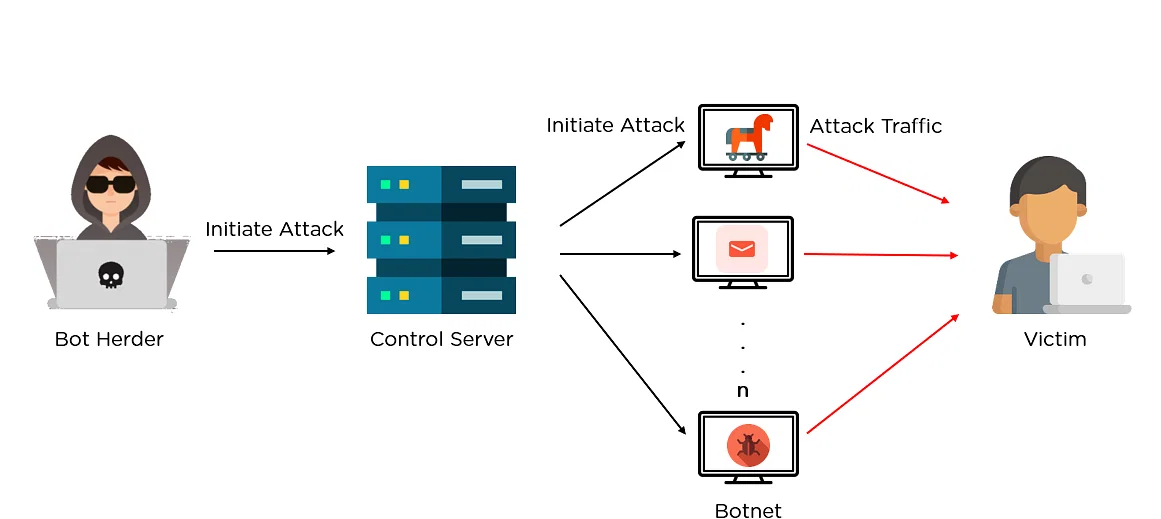
\includegraphics[width=8cm]{Botnet_1.jpg}
    \caption{esempio di architettura di una Botnet \cite{BotnetExampleImage}.}
    \label{fig:botnetexample}
\end{figure}
Le Botnet possono essere di tipo \textit{push based} o \textit{pull based}. Nel primo caso è il server che invia i comandi al bot mentre nel secondo caso è il bot infetto che è incaricato di richiedere i comandi al server periodicamente.
 La modalità operazionale  dipende più che altro dal protocollo in uso\footnote{eg. HTTP costruito su modello richiesta-risposta quindi una Botnet basata su questo protocollo sarà di tipo pull based.}.
 Di seguito verranno presentati i principali schemi comunicazioni, topologie, protocolli e tecniche di occultamento delle Botnet \cite{vormayr2017botnet,vuong2011advanced}.


\section{Schema Comunicazionale}
Parte importante della comunicazione della Botnet è il \textit{coordinamento}. I task che non sono automatizzati vengono eseguiti solo dopo aver ricevuto l'apposito comando dal C\&C, il che implica una serie di messaggi da e verso il server. I task automatizzati non richiedono il coordinamento con il server di controllo e quindi non generano traffico di rete. Di conseguenza più sono i task automatizzati, meno sarà il traffico di rete necessario per la coordinazione del bot e più sarà difficile da identificare la Botnet attraverso l'analisi del traffico di rete. Ovviamente limitare il coordinamento è a discapito della flessibilità, quindi solo una parte dei task viene automatizzata (ovviamente ci sono eccezioni anche a questo). 

Lo schema di comunicazione della Botnet può essere separato in più parti: \textit{propagazione} e \textit{operazione}. Questi passi, dal punto di vista dell'host compromesso, possono avvenire solo sequenzialmente dato che l'infezione deve avvenire prima che il bot possa divenire operazionale. 
\subsection{Propagazione}
La parte di \textit{propagazione} è la fase in cui si cerca di reclutare nuovi bot. È la prima fase in nel ciclo di vita di un bot, ed è una fase importante dato che la potenza di una Botnet aumenta con la sua grandezza\footnote{eg. Botnet capace di attacchi DDoS è più efficiente se ha più bot attraverso il quale generare traffico di rete.}. Un'eccezione a questo sono gli APT (Advanced Persistent Threat) che sono attacchi mirati solitamente, e quindi necessitano solo di un limitato numero di macchine, oltre al fatto che devono rimanere nascoste nel sistema il più a lungo possibile, evitando dunque di propagarsi per non rischiare di essere rilevate.

La propagazione può avvenire attivamente o passivamente.
Entrambi i metodi di propagazione implicano che l'host vittima venga infettato con l'eseguibile di riferimento della  Botnet. 
\subsubsection{Attiva}
\label{PropagazioneAttiva}
Nella propagazione attiva, il bot cerca e sfrutta vulnerabilità in altre macchine per espandersi. Questo può avvenire su comando del C\&C o in automatico. A seconda dell'\textit{exploit}\footnote{codice usato per sfruttare una vulnerabilità.} selezionato, una prima fase di scansione della rete può essere necessaria.


Una volta che la macchina è infetta, se il task non è automatizzato sarà necessario una messaggio di coordinazione dal C\&C server, in cui si specificano parametri per l'exploit e la possibile scansione di rete, oltre ad avviare l'infezione. Alcune Botnet mantengono questi parametri di configurazione in binario o in file separato, non necessitando dunque di un passo di coordinazione. 

La scansione di rete è opzionale, e può essere di diversi tipi a seconda delle informazioni che si vuole ottenere e del livello di occultamento che si vuole mantenere. Ad esempio potrebbero essere usate scansioni UDP\footnote{User Datagram Protocol.}/TCP\footnote{Transmission Control Protocol.} per cercare servizi esposti e vulnerabili, o semplicemente richieste ICMP\footnote{Internet Control Message Protocol.} per limitarsi a identificare quali porte sono attive sull'host target.


Lo step principale è l'infezione, in cui si cerca di abusare i  servizi vulnerabili della macchina vittima. Questa fase dipende molto dal tipo di attacco scelto\footnote{eg. eseguire una richiesta contenente un payload maligno o eseguire attacco \textit{bruteforce}\footnotemark su un servizio (eg. \textit{ssh}).}
\footnotetext{attacco in cui si cerca di indovinare una combinazione in modo esaustivo, testando tutte le combinazioni possibili.}.
Dato che durante questa fase la dimensione di dati scambiabili è relativamente limitata, una fase ulteriore di \textit{download} può essere necessario.


\label{Download}Il download può avvenire in più parti, tipica delle \textit{multi stage infection}. In primo luogo la vittima esegue solo un piccolo eseguibile\footnote{un eseguibile di piccole dimensioni è solitamente meno sospetto.} detto \textit{dropper} che si occupa di rimediare l'eseguibile vero e proprio dalla Botnet o da un'altra sorgente. Il binario può anche essere ricevuto criptato, rendendo ulteriormente difficile per i ricercatori riuscire a ottenere l'eseguibile per scopi di \textit{reverse engineering}\footnote{tecnica di analisi di un binario attraverso appositi strumenti, necessario per capire il flusso di esecuzione di un programma e relative funzionalità senza eseguirlo.}. Quindi l'eseguibile viene opzionalmente decriptato ed eseguito.

La fase finale di questo processo di propagazione attiva è lo step di \textit{registrazione}.
Questo step è opzionale, ma fondamentale se si vuole tener traccia delle dimensioni della Botnet, in caso di Botnet \textit{push based}\footnote{il server deve conoscere la posizione del bot per poter comunicare con esso.} o per particolari tipologie di Botnet\footnote{eg. Botnet P2P.}.

\subsubsection{Passiva}
Con propagazione passiva si intende la distribuzione del malware di riferimento attraverso altri vettori non in controllo della Botnet. Questo include propagazione attraverso email, siti web o dispositivi di archiviazione esterna. Comune a questi meccanismi di infezione è il fatto che la vittima infetta la propria macchina eseguendo il malware, attraverso un click o un azione particolare. 
La distribuzione via email può avvenire attraverso email di \textit{phishing}. Queste sono email che sembrano legittime, ma che in realtà hanno l'obiettivo di ingannare la vittima ad aprire un file allegato o visitare un particolare sito web maligno. Analoghi a email di phishing sono i siti web di phishing. Pagine web uguali alla loro copia legittima ma appartenenti a domini diversi (tecnica anche detta \textit{domain typosquatting}).

Si possono anche usare vulnerabilità in browser, plugin della vittima o compromettere un sito web che esso visita frequentemente, per causare un \textit{drive by download}\footnote{tecnica di attacco che si riferisce al download non intenzionale di software maligno da sito compromesso.}.

Si noti che in un contesto del genere, solo la ricezione di un email o la visita a un sito web può essere individuata a livello di rete. Inoltre la comunicazione in questo caso usa gli stessi protocolli e modalità del traffico di rete legittimo. Per questo motivo solo attraverso Deep Packet Inspection\footnote{analisi dei pacchetti di rete che va oltre alla mera intestazione.} (DPI) sarebbe possibile individuare contenuto eseguibile e questo è possibile solo se il tutto non è criptato.

Dispositivi di archiviazione esterna possono essere infettati per far sì che il malware si muova tra dispositivi. All'inserimento del media di archiviazione all'interno di un altro \textit{device}, questo avrebbe una copia dell'eseguibile potenzialmente eseguibile, senza alcun traffico di rete o movimenti sospetti.

Una volta che il malware viene eseguito sulla macchina vittima, seguono le fasi di download e registrazione, opzionali e comuni alla propagazione attiva (\Cref{PropagazioneAttiva}).


\subsection{Operazione}
 La seconda fase è quella \textit{operazionale} in cui si eseguono i veri e propri \textit{task}, a seconda di quali siano gli obiettivi della Botnet. I task possono essere categorizzati in accordo al loro obiettivo come: 
\begin{itemize}
    \centering
    \item Download  dati;
    \item Upload  dati;
    \item Forward Proxy;
    \item Reverse Proxy;
    \item Instruction.
\end{itemize}

\subsubsection{Download dati}
Con Download ci si riferisce alla memorizzazione di dati in bot, provenienti da sorgenti esterne. Dati possono essere file arbitrari, aggiornamenti della Botnet o malware aggiuntivo. I dati potrebbero perfino essere contenuti illegali atti a screditare la vittima. Questo meccanismo permette anche di offrire la Botnet come servizio di distribuzione di malware a pagamento. In questo modo sviluppatori di malware possono pagare il botmaster per avere un base di partenza di macchine su cui poter installare in modo agile il proprio software maligno.

La capacità di aggiornamento della Botnet permette di adattare la rete a nuove necessità oltre che a difendersi da possibili minacce. Ovviamente questa capacità deve essere ben progettata in quanto può fornire un vettore di attacco a terzi, che possono sfruttare questa \textit{feature} per prendere possesso della Botnet o per rimpiazzarla con un altra.

L'operazione di Download inizia con una prima parte di coordinazione in cui si specifica quale file scaricare e dove cercarlo. Infatti il bot non è costretto a scaricare il file dal C\&C server, che quindi non necessita di incorporare meccanismi e protocolli di \textit{file transfer}. Il bot potrebbe avere all'interno del binario delle direttive di download da eseguire subito dopo l'infezione, rendendo la fase iniziale di coordinazione  superflua.
I dati possono anche essere passati all'interno del messaggio di coordinazione o essere inclusi in binario in fase di propagazione, in caso contrario verranno scaricati successivamente.

L'ultima fase è quella in cui si memorizzano i dati in macchina o dove si esegue il software aggiuntivo scaricato, a cui può seguire un messaggio opzionale verso il server.

\subsubsection{Upload dati}
L'operazione di Upload dati dal bot verso il server viene utilizzata da tutte quelle tipologie di Botnet che hanno come scopo ultimo la raccolta di dati o il calcolo distribuito.
Con raccolta di dati si intende prelevare informazioni dal sistema infetto. Queste informazioni possono essere file arbitrari, informazioni sensibili dell'utente, credenziali d'accesso, informazioni del sistema in uso, etc.
Con calcolo distribuito si intende l'upload del risultato di una computazione eseguita in modo distribuito su tutti i nodi infetti della rete.

Questo task inizia con uno step di coordinazione, in cui il C\&C server invia comandi con specifiche istruzioni o dati se necessari, che può essere opzionale nel caso l'upload venga eseguito subito dopo la propagazione. 
Successivamente i dati richiesti sono prelevati dal bot o la computazione richiesta è eseguita. 
Per concludere i dati sono inviati al server.
\subsubsection{Forward Proxy}
Un \textit{forward proxy} è un server capace di connettersi a un  host specifico come tramite per un altro host.
Questo permette di mantenere l'anonimato dell'host che inizia la richiesta, di fare tunneling  delle connessioni o di effettuare connessioni verso host che altrimenti non sarebbero raggiungibili.

Le Botnet possono implementare proxy unidirezionali o bidirezionali. 
Proxy bidirezionali sono necessari se si vuole il risultato di una richiesta. Alcune Botnet includono SOCKS proxy\footnote{proxy server in grado di eseguire forward di connessioni TCP e UDP (da versione 5 in poi) indipendentemente dal protocollo applicativo veicolato.}  come servizio, permettendo di utilizzare la Botnet come servizio di anonimato, sfruttando  i bot come proxy server generici.
Altro  uso di proxy bidirezionale è la possibilità di valicare Firewall o NAT infettandoli e usandoli come proxy, fungendo da \textit{bridge} verso i device interni alla rete che altrimenti non sarebbero raggiungibili.

Per creare meno traffico sospetto possibile, la Botnet può anche usare i proxy per fare \textit{protocol encapsulation}, ovvero nascondere un protocollo all'interno di un altro. In questo modo i sistemi di rilevazione devono fare lo sforzo aggiuntivo di essere in grado di interpretare tutti i protocolli possibili se voglio ricostruire la comunicazione originale.

Proxy unidirezionali possono essere usati per effettuare attacchi DDoS. Infatti il botmaster non ha bisogno di controllare ogni messaggio e non è interessato alla risposta di questi. Gli basta comunicare destinazione e il tipo di comunicazione da utilizzare.

Un altro modo di usare i proxy unidirezionali è quello di usarli per distribuire email di spam. Durante la fase di coordinazione al  master basta invia il \textit{template} della email e una lista degli host da colpire.

A livello di schema comunicazionale, sia quello unidirezionale che bidirezionale iniziano con uno step di coordinazione.
Nel caso bidirezionale viene settata la configurazione del proxy con le porte su cui fare \textit{forwarding} e i protocolli da usare. Dato che queste configurazioni possono essere già incluse in binario questo step è opzionale.

Per il proxy unidirezionale invece, che è usato esclusivamente per eseguire task automatizzati, questo passo non è opzionale. Ad esempio se si vuole eseguire un attacco DDoS deve essere impostato il tipo di attacco, il target e la durata. In teoria, potrebbe essere possibile inserire tali informazioni nel codice binario, ma ciò potrebbe rendere questo tipo di attacco troppo rigido, mentre esso per natura richiede di essere improvviso e di durata variabile.

L'ultimo step è lo scambio di dati. In caso il proxy sia bidirezionale, la comunicazione sarà composta di richieste e risposte dove il bot farà da tramite.  Nel caso di proxy unidirezionale i dati sono inviati solamente da bot verso il target. 
\subsubsection{Reverse Proxy}
Le Botnet possono essere usate per creare un \textit{fast-flux network} (\Cref{fast-flux-network-label}). Un \textit{fast-flux network} consiste di più \textit{reverse proxy server}\footnote{mentre un forward proxy server funge da intermediario per un client, il reverse proxy server agisce come intermediario per il server, ponendosi tra il client e il server.} che sono usati per connettersi al C\&C server.Dato che le connessioni sono verso i proxy, l'identità del C\&C server rimanere nascosta, rendendo il server più resistente a possibili \textit{take down}.

La comunicazione di rete necessaria per questo task inizia con uno step di coordinazione in cui il bot è istruito di quali porte aprire e verso quali indirizzi interni connettersi. Dopo questa fase di coordinazione altri host o bot possono connettersi al reverse proxy per comunicare indirettamente col C\&C server. Le informazioni di coordinazione non sono preinseribili nel binario del malware per via della natura della Botnet. I bot che fungono da reverse proxy potrebbero infatti  non essere mai raggiungibili  in uno scenario in cui gli indirizzi di questi dovessero essere prefissati\footnote{I bot potrebbero non essere online, il malware può essere neutralizzato o possono esserci problemi di rete.}.

\subsubsection{Instruction}
Una delle feature presenti nelle Botnet è la capacità di eseguire task a nome del botmaster che non generano traffico di rete. Esempi di task di questo genere sono: 
\begin{itemize}
    \item Terminazione di  altri processi;
    \item Cancellazione di  file;
    \item Modifiche al  traffico di rete dell'host;
    \item \textit{Disruption} di  servizi;
    \item Creazione di  \textit{backdoor}\footnote{rendere la macchina accessibile dall'attaccante attraverso la  rete.};
    \item Distruzione o criptazione di dati in dispositivi di archiviazione;
    \item Esecuzione di eseguibili.
\end{itemize}

La comunicazione necessaria per questo genere di operazione inizia con una fase di coordinazione in cui vengono specificati il task da eseguire ed eventuali parametri. Gli eseguibili della Botnet possono essere accompagnati da file di configurazione contenenti queste istruzioni o possono essere inclusi in binario direttamente, rendendo questa fase opzionale. Ad esempio molte Botnet contengono una lista dei processi di antivirus da chiudere o disabilitare. Dopo lo step di coordinazione vengono eseguiti i comandi ricevuti.
\section{Topologie di rete}
La comunicazione tra C\&C server e i bot può essere organizzata da un punto di vista topologico nei seguenti modi:
\begin{itemize}
    \item Centralizzata;
    \item Decentralizzata;
    \item Ibrida.
\end{itemize}

\subsection{Centralizzata}
Nella topologia centralizzata ogni bot si connette direttamente a un unico server.
Per una topologia del genere spesso sono usati protocolli di comunicazione semplici come Internet Relay Chat (IRC) (\Cref{IRC}) o HyperText Markup Language (HTTP). Per questo motivo ne risulta anche semplificato il \textit{set-up}, dato che questi protocolli non hanno particolari esigenze da soddisfare. 
Una topologia del genere gode anche di bassa latenza, dato che bot e server si scambiano messaggi direttamente, e di alta scalabilità per via della semplicità della rete. 

Tuttavia questa semplicità di rete è a discapito della robustezza. Infatti una struttura centralizzata ha un singolo \textit{point of failure} e il \textit{take down} del server principale di comando e controllo comporterebbe la rottura dell'intera rete Botnet. 
Il singolo \textit{point of failure} può essere mitigato in parte utilizzando più C\&C server.
Un'altra tecnica utilizzata per mitigare il problema della robustezza è il \textit{fast-flux} che verrà descritto nella \Cref{fast-flux-network-label}.

Altro punto a sfavore di questa topologia è il fatto che gli indirizzi dei C\&C server devono essere inseriti all'interno del binario del bot. Questo è un rischio per il botmaster che potrebbe perdere il controllo del C\&C server in caso questi indirizzi dovessero essere scovati da un'analista di sicurezza informatica.
Una possibile soluzione potrebbe essere criptare od offuscare il codice del bot. Tuttavia anche questa soluzione risulterebbe temporanea in quanto non garantirebbe la sicurezza che questi indirizzi non vengano trovati a seguito di un analisi approfondita da parte di uno specialista.
Una tecnica spesso usata per evitare l'\textit{hardcoding} degli indirizzi dei server è il Domain Generation Algorithm (DGA) che verrà analizzato nella \Cref{DGA}.

\subsubsection{Fast-flux network}
\label{fast-flux-network-label}
In un Fast-flux network il servizio Domain Name System (DNS) di risoluzione degli \textit{hostname} viene usato come \textit{multiplexer} e \textit{load balancer}. La macchina infetta non comunica direttamente col server usando il suo indirizzo IP ma punterà a risolvere un hostname attraverso risoluzione DNS. Al record DNS in cui vi è registrato l'hostname da risolvere saranno associati molteplici indirizzi IP appartenenti a più bot della Botnet. Così facendo si sfrutta le capacità native di \textit{load balancing} dei server DNS per ciclare sugli indirizzi IP assegnati. I bot così associati a questo hostname sono gli unici a conoscenza dell'indirizzo IP del C\&C server e quindi sono gli unici in grado di comunicare con esso. 
Quando una macchina infetta ha necessità di comunicare con il server di controllo, risolve l'hostname associato ottenendo l'indirizzo IP di un bot che farà da proxy (reverse proxy) nella comunicazione verso il server.
In questo modo  si sposta il singolo point of failure dal server C\&C al DNS server.

Per rendere più complessa la rete ed eliminare anche questo point of failure si può creare un  \textit{double-flux} network. Il double-flux usa lo stesso schema per ciclare i \textit{name server} autoritativi che risolveranno l'hostname richiesto, traducendolo come visto in uno dei bot che farà da proxy verso il C\&C server. 

Si noti che registrare ed eliminare un  record DNS sono operazioni veloci e quindi è possibile variare velocemente i bot che fungono da proxy o name server.

Anche utilizzando questa tecnica rimane comunque il problema dell'hardcoding degli hostname all'interno del binario del bot. Per risolvere anche questo problema spesso  questa tecnica viene associata a \textit{Domain Generation Algorithm} (DGA) che verrà di seguito descritto.

\subsubsection{Domain Generation Algorithm (DGA)}
\label{DGA}
Domain Generation Algorithm è un algoritmo utilizzato per creare domini partendo da un valore di input variabile \cite{inproceedings}. Molte Botnet usano questo algoritmo per generare e registrare in automatico questi domini per il loro C\&C Server.

Quando il bot vuole cercare di contattare il server, usa l'algoritmo per generare un numero significativo di domini che proverà a risolvere. Il master che è a conoscenza dei dettagli dell'algoritmo, può preregistrare uno dei domini generati per essere contattato con successo dai bot.
Così facendo non è necessario preinserire domini all'interno dell'eseguibile.  Molti DGA usano il tempo corrente come input, rendendo necessario che ogni bot abbia l'orologio di sistema sincronizzato per poter funzionare correttamente. 
Se per esempio un bot dovesse generare 50.000 domini da testare, un ente governativo dovrebbe preregistrare tutti i 50.000 domini per poter evitare che il botmaster riesca nel suo intento. Inoltre va considerato che se le comunicazioni tra bot e server dovessero usare cifratura a chiave pubblica, anche preregistrando correttamente uno dei domini che la Botnet usa per coordinare i bot, non si riuscirebbe a prenderne il controllo in quanto la comunicazione verrebbe negata per via delle firme digitali non combacianti con quelle del botmaster.

Un esempio di algoritmo DGA può essere il seguente \cite{inproceedings}:

\begin{algorithmic}[1]
    \State $i \gets 0$
    \State $domain \gets \:  '\;'$
    \State $year, month, day \gets getCurrentDate()$
    \While{$i<16$}
        \State $year \gets ((year \; ^  \wedge \; 8 \cdot year) >> 11) \; ^\wedge \; ((year \: \& \: \texttt{0xFFFFFFF0}) << 17) $
        \State $month \gets ((month   \;^ \wedge \; 4 \cdot month) >> 25) \; ^ \wedge \; 16 \cdot (month \: \& 
 \: \texttt{0xFFFFFFF8}) $
        \State $day \gets ((day \;^ \wedge \;(day << 13)) >> 19) \;^\wedge \; ((day \:\& \:\texttt{0xFFFFFFFE}) << 12) $
        \State $domain \gets domain + chr(((year ^\wedge month ^\wedge day) \% 25) + 97) $
    \EndWhile
\end{algorithmic}

\subsection{Decentralizzata (P2P)}
\label{TopologiaDecentralizzata}
Una topologia decentralizzata è tipica di una rete di soli bot dove ogni bot può essere un potenziale C\&C Server. Questo meccanismo in cui qualsiasi nodo può potenzialmente essere server è tipico delle reti Peer-To-Peer (P2P).
Ogni bot è connesso ad almeno un altro bot e i comandi del C\&C possono raggiungere ogni nodo della rete se ogni bot ha l'abilità di passare i comandi ai nodi direttamente connessi.


Una rete decentralizzata può essere a maglia parzialmente connessa o completamente connessa.

Una topologia a maglia completamente connessa ha il vantaggio di essere a bassa latenza dato che i comandi non devono essere passati a nodi intermedi per arrivare a tutti i nodi. Un altro vantaggio è che una rete del genere risulta molto robusta in quanto togliere un numero arbitrario di nodi non influenza negativamente la comunicazione di rete degli altri nodi. Tuttavia, considerando che questa topologia richiederebbe un altro numero di connessioni per una rete composta di molti nodi, risulterebbe non scalabile. I sistemi operativi infatti hanno limiti sul numero di connessioni che possono aprire e quindi viene limitato il numero massimo di bot in rete. Inoltre il numero di connessioni influisce sulla visibilità in rete della Botnet. Aggiungere e togliere nodi alla rete necessita di un alto numero di messaggi di coordinazione e per questo motivo spesso le Botnet P2P non sono a maglia completamente connessa.

Una topologia a maglia parzialmente connessa non ha i problemi delle topologie a maglia completamente connessa appena visti ma ha comunque dei fattori negativi. 
Dato che un bot non è connesso a tutti gli altri bot, l'eliminazione di nodi topologicamente importanti dalla rete può causare la completa interruzione delle comunicazioni per una parte dei device connessi.
Implementare topologie P2P risulta difficile a causa principalmente del dover garantire una distribuzione affidabile dei comandi verso tutti i bot oltre al problema di trovare i \textit{peer} iniziali.

Il problema della ricerca iniziale dei peer può essere ovviata inserendo la lista in eseguibile di bot. Un altro modo è quello di usare tecnologie pubbliche già esistenti per memorizzare e in seguito reperire la lista di peer (eg. usare cache server di applicazioni P2P esistenti). Il point of failure della rete si sposta così alla lista di peer iniziali. Un'altra alternativa alle liste di peer pubbliche è la possibilità di scansionare l'intera rete Internet in cerca di peer.

Dato che la rete non è a maglia completa, deve anche essere garantito il trasporto affidabile dei comandi che in questo caso non è nativo di questa topologia di rete. Per questo motivo spesso si usano protocolli P2P già noti che hanno questa funzionalità già implementata. Se si vuole creare la Botnet attraverso un protocollo \textit{ad-hoc}, le funzionalità di consegna affidabile dei messaggi e di \textit{routing} devono essere implementate per poter garantire il corretto funzionamento della rete.

Dato che non tutti i dispositivi sono direttamente raggiungibili da Internet a causa di possibili Firewall o NAT, spesso le Botnet classificano i bot in due categorie: \textit{super node} e \textit{NAT-node}.
A seguito dell'infezione la connettività viene rilevata e solo i NAT-node sono usati per attività maligne mentre i super node sono usati solo come tramite per le comunicazioni con i bot C\&C.

\subsection{Ibrida}
Uno dei modi per ovviare alle problematiche di una rete decentralizzata e allo stesso tempo di fruire dei vantaggi che offre come topologia, è quello di combinarla con la topologia centralizzata per avere i vantaggi di entrambe.
Invece di connettere direttamente i bot al C\&C server, un livello di proxy viene aggiunto. Questo livello di proxy è costituito da bot connessi in P2P. 

I bot che eseguono i task costituiscono un ulteriore livello. 

L'assegnamento di un bot al ruolo di worker o proxy è eseguito considerando le proprietà di connettività dei bot analizzati.

Per aumentare ulteriormente la sicurezza del C\&C Server si potrebbe aggiungere un ulteriore livello di proxy a discapito di una maggiore latenza.

Altre  Botnet ibride sono possibili sfruttando topologie diverse per task diversi. Una Botnet potrebbe ad esempio sfruttare topologia P2P per lo scambio di messaggi e topologia centralizzata con un web server per il download di dati.

\section{Protocolli}
Di seguito verranno brevemente descritti i protocolli più comunemente usati a livello comunicazionale e operazionale nelle Botnet. 
\subsection{Protocolli Comunicazionali}
Con Protocolli comunicazionali si intende quei protocolli usati all'interno della Botnet per la comunicazione tra bot e Server, all'interno di una rete centralizzata, o tra bot e bot all'interno di una Botnet P2P.
Ovviamente la scelta della topologia pone restrizioni sulle possibilità di scelta del protocollo comunicazionale.

Le Botnet spesso usano protocolli già esistenti, semplificando lo sviluppo della rete.

Il protocollo scelto può anche essere creato su misura. Questo permette di soddisfare  esigenze specifiche come un maggior mimetismo\footnote{eg. si potrebbe creare un protocollo che mimi il traffico legittimo.}  o restrizioni di rete\footnote{eg. molte reti di corporazioni non permettono l'uso di particolari tipi di protocolli.}.

\subsubsection{Internet Relay Chat (IRC)}
\label{IRC}
Internet Relay Chat  è un protocollo a livello applicativo di messaggistica \textit{text-based}, basato su architettura client-server. Venne inizialmente creato  per lo sviluppo di applicazioni chat su Internet \cite{rfc1459}, in particolare inizialmente usato su Bulletin Board System (BBS)\footnote{sistema telematico client-server creato negli anni '70 prima che i Web Browser venissero realizzati. L'utente si connetteva a un server centrale per condividere e prelevare risorse.}.
IRC inizia a essere sviluppato nell'anno 1989. Nell'anno 1993 J.Oikarinen pubblica l'RFC 1459 in cui vengono pubblicate le specifiche del protocollo.

Il client comunica con il Server che è responsabile di consegnare i messaggi ad altri client e server.
Messaggi possono essere scambiati  client-client o verso un gruppo di client attraverso \textit{canali}\footnote{gruppo di client a cui viene assegnato un nome. Un messaggio verso un canale arriva a tutti i client appartenenti al gruppo rappresentato.}. I canali possono essere protetti da password. 

Il protocollo supporta anche il trasferimento di file.

Questo protocollo facilita lo sviluppo di una Botnet basata su topologia centralizzata. Il botmaster ad esempio potrebbe inviare i comandi verso un canale di bot, dove il C\&C in questo caso ricopre il ruolo di Server centrale incaricato di distribuire il messaggio a tutti i bot interessati. I canali come già detto, possono essere protetti da password per evitare che terzi prendano il controllo della Botnet. La capacità di file-transfer può essere sfruttata per distribuire malware, aggiornamenti della Botnet, file di configurazione, etc.

Tra gli svantaggi di questo protocollo ci sono il fatto che è facilmente identificabile e che non è un protocollo che viene comunemente usato nelle attività di tutti i giorni (nonostante sia un protocollo molto diffuso su Internet) e quindi potrebbe essere bloccato preventivamente via Firewall\footnote{Spesso questo è il caso delle reti corporative.}.

\subsubsection{HTTP}
\label{HTTP}
Uno dei protocolli a livello applicativo più utilizzati su Internet. Usato per la trasmissione di pagine web da web server a web client su Internet. È basato su architettura client-server dove la comunicazione di gruppo, al contrario di IRC, non è possibile. Visto il largo uso nella rete Internet, sono presenti tantissime implementazioni già pronte di client e server, rendendo lo sviluppo di una Botnet basata su protocollo HTTP facilitata.

Vista la struttura di HTTP può essere usato agilmente per creare una Botnet con topologia centralizzata.

Implementando un HTTP server e un HTTP client su ogni bot è possibile creare una rete P2P.
Nonostante questo sia possibile attraverso HTTP, si dovrebbe comunque risolvere alcuni dei problemi noti alle reti P2P come rendere la comunicazione tra bot affidabile e la gestione dei messaggi replicati.
Una possibile soluzione può essere creare dei \textit{layer di rete}   aggiuntivi sopra HTTP.
Si potrebbe creare quindi un livello P2P per aggiungere informazioni necessarie per il trasporto affidabile dei messaggi a ogni nodo e per prevenire messaggi replicati.
Un altro livello di routing opzionale potrebbe essere implementato per gestire l'invio selettivo di un messaggio a uno specifico bot non conoscendo il percorso esatto all'interno della rete P2P. Con il livello di routing si potrebbe anche implementare il trasporto affidabile, rendendo opzionale il livello P2P precedentemente descritto.


All'interno di questi livelli aggiuntivi si potrebbe anche aggiungere la possibilità di far rimbalzare il messaggio tra un numero arbitrario di nodi prima di consegnare il messaggio a destinazione, rendendo più complessa l'identificazione dell'origine del messaggio. Questa tecnica è nota col nome di Stepping Stones (\Cref{TecnicheOccultamento}).

Il fatto che HTTP sia largamente utilizzato su Internet rende lo scambio di messaggi attraverso questo protocollo non sospetto.

La sua variante  HTTPS permette l'uso di comunicazione HTTP all'interno di una connessione cifrata, rendendo quasi\footnote{i firewall posso usare una tecnica chiamata \textit{HTTPS interception} dove si sfrutta lo stesso principio degli attacchi Man In The Middle (MITM)\footnotemark{} \footnotetext{attacco informatico in cui l'attaccante si frappone tra la sorgente e la destinazione della comunicazione di rete, permettendogli potenzialmente di leggere/modificare/eliminare i pacchetti intercettati.} per analizzare il contenuto dei pacchetti HTTPS.} impossibile analizzare il contenuto dei messaggi da parte di strumenti di rilevazione.

\subsubsection{Server Message Block}
Server Message Block (SMB) è un protocollo  originariamente specificato da Microsoft, IBM e Intel per la condivisione di file, stampanti, porte seriali e comunicazioni di varia natura attraverso la rete \cite{SMB}.

Basato su architettura client-server. Un client si connette a un server autenticandosi con credenziali utente o come anonimo. Una volta connesso può richiedere una lista di \textit{share} disponibili. Con \textit{share} si intende una lista di file o servizi accessibili.

SMB implementa anche meccanismi di comunicazione tra processi via network.

Questo protocollo può anche essere usato per infettare passivamente altri host. Se infatti un file condiviso è modificabile, un utente malintenzionato potrebbe inserire codice maligno all'interno di questo  che in seguito  potrebbe venir eseguito da un utente ignaro (propagazione passiva) in seguito al download  sulla propria macchina.

Questo protocollo spesso viene bloccato dai \textit{gateway} che provvedono accesso a Internet, motivo per cui viene principalmente usato dalle Botnet come protocollo di comunicazione in rete locale.

\subsubsection{Protocolli P2P}
Come già detto nella sezione inerente le topologie decentralizzate di Botnet (\ref{TopologiaDecentralizzata}), i protocolli P2P esistenti vengono spesso adottati per evitare di dover sviluppare protocolli P2P da zero. Questi protocolli possono  essere usati per creare una rete P2P separata o per nascondere la rete di bot all'interno di una rete P2P esistente.
Un esempio di protocollo usato è WASTE \cite{WASTE}, originariamente creato come protocollo di messaggistica distribuita e file sharing. Un altro esempio di protocollo usato è Kademlia \cite{maymounkov2002kademlia}, che gestisce la struttura della rete, la comunicazione tra nodi e il modo in cui lo scambio di informazioni è effettuato.

\subsubsection{Protocolli ad-hoc}
La creazione di un protocollo \textit{ex novo} permette di creare una comunicazione su misura che rispecchi le esigenze e gli obiettivi che la Botnet vuole perseguire. 

La maggior parte dei protocolli creati appositamente risulta basata su UDP o TCP a livello di trasporto. Ci sono anche casi osservati di protocolli basati su ICMP. Come già discusso precedentemente a seconda della topologia scelta  si devono implementare tutte le accortezze necessarie al corretto funzionamento della rete. 

Se si desidera una rete P2P è necessario implementare la comunicazione affidabile dei messaggi e gestire i messaggi duplicati. La questione dei messaggi duplicati può essere ovviata associando un identficativo (ID) ai comandi.
Il trasporto affidabile dei messaggi deve essere gestita anche nel caso si utilizzi UDP come protocollo a livello di trasporto. Questo può essere garantito ad esempio implementando ritrasmissione dei messaggi e l'invio di acknowledgment.
Un protocollo basato su UDP con consegna affidabile dei messaggi avrebbe anche il vantaggio di poter permettere più connessioni contemporaneamente in quanto nessuna connessione deve essere mantenuta al contrario di TCP.

Il payload dei messaggi può essere in binario o testo. Un payload formato testo necessita di un \textit{parser} per comprendere i comandi così codificati, oltre a essere più facile da analizzare a livello di reverse engineering.

Uno dei punti a sfavore dei protocolli creati su misura è che questi non sono usati all'interno di traffico di rete legittimo e quindi potrebbe essere identificato.

\subsection{Protocolli Operazionali}
Oltre ai protocolli usati per il normale funzionamento della Botnet, sono necessari anche altri protocolli per svolgere i task operazionali atti a  raggiungere l'obiettivo preposto. 
Di seguito verranno presentati alcuni esempi di  protocolli usati per le più comuni attività  di una Botnet:

\begin{itemize}
    \item Per inviare spam via email deve essere in grado di poter usare  Simple Mail Transport Protocol (SMTP). SMTP è un protocollo slient-server usato per inviare messaggi di posta elettronica attraverso server dedicato (Server SMTP). Dato che molti server di posta elettronica richiedono autenticazione solo per inviare messaggi fuori dalla rete locale, questa risulta la principale causa di spam. Un bot potrebbe infatti sfruttare la sua posizione all'interno della rete per inviare email di spam attraverso il mail server comune, verso altri nodi della rete locale. Per questo motivo molti email provider bloccano email provenienti da IP di reti private;
    \item HTTP e HTTPS vengono usati per eseguire \textit{click fraude}, ovvero simulare il click su un URL o  annuncio pubblicitario col fine di alterarne le statistiche di visita della risorsa. In questo modo il botmaster può fare profitto grazie al numero falsato di visite all'annuncio o pagina web;
    \item HTTP, UDP e TCP vengono anche usati per eseguire attacchi DDoS in cui si cerca di sovraccaricare il network del servizio target. Un altro modo di sovraccaricare il servizio è attraverso l'invio di richieste computazionali intensive con l'intento di saturare la capacità di calcolo dell'applicazione target.
\end{itemize}


\section{Tecniche di occultamento e offuscamento di comunicazione}
\label{TecnicheOccultamento}
Di seguito verranno brevemente raccolte alcune delle tecniche usate dalle Botnet per nascondere le comunicazioni od offuscarne il contenuto. Con offuscamento si intende rielaborare il contenuto in modo che risulti complesso comprenderne il significato, usato spesso per rendere più difficili i tentativi di reverse engineering o di analisi.

\subsection*{Canali nascosti}
 Considerando che, come  già detto, i protocolli costruiti ad-hoc sono facilmente individuabili in quanto non figurano comunemente nella rete Internet e che i protocolli già esistenti generano traffico di rete che non dovrebbe esistere in scenario normale,  si possono usare i canali nascosti per occultare la comunicazione.
  Con canali nascosti si intende instaurare una comunicazione sfruttando mezzi che non sono usati a scopo comunicativo. Un esempio è usare gli header dei segmenti TCP o dei datagrammi del protocollo IP per comunicare informazioni o comandi. 

 \subsection*{Crittografia}
 L'ispezione del contenuto del traffico di rete permette la ricerca di pattern di messaggi  di Botnet conosciute, portando a una possibile identificazione dei device infetti o del C\&C server. 
 Per questo motivo spesso le Botnet usano crittografia a livello di rete per fare in modo che terzi non riescano a ispezionare il contenuto delle comunicazioni. 

 Un esempio di protocolli usati a tal fine sono HTTPS o TLS. Sebbene sia possibile creare protocolli crittografici su misura, ciò pone il rischio che una falla nel protocollo crittografico lo renda completamente inefficace. Per questo motivo i botmaster devono preoccuparsi di usare protocolli aggiornati che non presentino vulnerabilità note nel caso decidano di utilizzare protocolli già esistenti.

 \subsection*{Molteplici protocolli}
 Per adattare il bot alla rete in cui risiede e quindi rendere la Botnet meno identificabile è possibile creare un livello di rete variabile capace di usare molteplici protocolli. Avendo una vasta scelta di protocolli, il bot potrebbe scegliere di usare quello più popolare all'interno della rete in cui risiede per rendere la comunicazione meno sospetta.

 \subsection*{Compressione}
 La compressione dei dati viene comunemente usata per ridurre la dimensione di file. Tuttavia nel comprimere i dati ne offusca anche il contenuto in quanto, nonostante l'informazione originaria rimanga intatta all'interno dei dati compressi, questi risultano non interpretabili a meno di conoscer l'algoritmo di decompressione.
 
 Dato che questa tecnica non richiede alcuna chiave, chiunque conosca l'algoritmo di compressione può  decomprimere i dati e quindi risalire al contenuto originario.

 \subsection*{Steganografia}
 La steganografia è un'altra tecnica di offuscamento. Essa consiste nel nascondere informazioni all'interno di \textit{contenitori} che non sono pensati per la comunicazione. Simile a livello di logica ai \textit{canali nascosti} ma che usa file (eg. immagini, video, documenti, etc.) per comunicare al posto degli attributi dei  pacchetti di rete.

 In passato sono state proposte Botnet capaci di sfruttare questo principio all'interno dei social network, incapsulando le informazioni dei comandi all'interno di immagini JPEG postate dall'utente \cite{nagaraja2011stegobot}.

 Altro esempio peculiare di botnet di questo tipo è quella ideata da A.Compagno e collaboratori, che hanno sfruttato i messaggi di testo all'interno dei social network, usando caratteri non visualizzati dai web browser \cite{nagaraja2011stegobot}.


 \subsection*{Stepping Stones}
 
 Tecnica usata per aumentare la segretezza del C\&C server che consiste nell'aggiungere un numero arbitrario di nodi intermedi tra il server e i bot destinatari dei comandi.  Questo può essere ottenuto implementando un layer di routing che permette di far rimbalzare i messaggi tra un numero desiderato di nodi prima di consegnarlo a destinazione.














 

\chapter{Infrastruttura di testing}
Prima di poter analizzare le botnet dinamicamente, è necessario progettare ed eseguire il \textit{deploy} di un infrastruttura  sicura, in cui è possibile eseguire i malware relativi alla botnet oggetto di studio senza rischiare di compromettere dispositivi al di fuori del perimetro designato.


Il deploy dell'infrastruttura è stato eseguito su un Server VMWare ESXi (\ref{esxi})  raggiungibile attraverso Virtual Private Network (VPN), in quanto situato all'interno della rete dell'Università di Bologna, Campus di Cesena. Attraverso le capacità di virtualizzazione del server sono state create una macchina Linux per ospitare il C\&C server e due macchine che verranno infettate con malware per trasformarli in bot attivi. Le macchine bot in questione sono una basata su Linux e l'altra su Windows.  Queste macchine sono assegnate a una rete VLAN isolata così che non siano in grado di comunicare con altri dispositivi al di fuori delle macchine soggette al test. Chiameremo questa rete \textit{botnet Vlan}.

Per far in modo che le macchine sotto testing potessero occasionalmente interfacciarsi alla rete Internet in modo controllato è stato aggiunto un Firewall (\ref{firewall}). La macchina in questione usa  ClearOs (\ref{ClearOS}) come sistema operativo e ha due Network Interface Card (NIC).
Una delle NIC è collegata a una VLAN connessa a Internet e ha indirizzo IP assegnatogli attraverso Dynamic Host Configuration Protocol (DHCP). L'altra NIC è collegata alla botnet Vlan e ha indirizzo IP statico assegnatogli manualmente. 

Una volta configurato il Firewall, le tabelle di routing dei bot e del C\&C server sono state modificate per fare in modo che il Firewall operasse da gateway per questi dispositivi. In questo modo quando i dispositivi all'interno della botnet Vlan cercheranno di comunicare all'esterno della rete il Firewall filtrerà le comunicazioni.

ClearOS ha diversi moduli installabili per configurare le funzionalità di Firewall. In questo caso è stato utilizzato un modulo basato su Iptables (\ref{iptables}).
    
Oltre alle funzioni di Firewall sono state usate le funzionalità di server DHCP che il sistema operativo offre attraverso modulo dedicato. Per mezzo di  questo sono stati assegnati gli indirizzi IP alle macchine interne alla botnet Vlan.

In seguito alla conferma della connettività  Internet delle macchine interne alla botnet Vlan,  sulle macchine Linux è stato installato per comodità un ambiente Desktop, di cui erano privi.

In fine per velocizzare il deploy dei nodi della botnet nelle rispettive macchine  e per facilitare il testing è stato installato Docker all'interno delle macchine della  botnet Vlan.

Per lo scambio di file con macchine fuori dal perimetro del server ESXi è possibile usare SSH Tunneling, a patto che il dispositivo interessato sia connessa alla stessa VPN del server.
    
Di seguito verranno descritte più nel dettaglio le principali tecnologie sopra citate.

\section{Server VMWare ESXi}
\label{esxi}
Il server sul quale sono stati effettuati i test usa  ESXi (Elastic Sky X integrated) \cite{esxi} sviluppato da VMWare come \textit{hypervisor bare metal} per la creazione e  gestione di macchine virtuali.


Un hypervisor, anche conosciuto come \textit{virtual machine monitor}, è un tipo di software di virtualizzazione che supporta la creazione e il management di macchine virtuali \cite{desai2013hypervisor,techtargetHypervisor}. Consente a un computer host di supportare diverse \textit{guest Virtual Machine (VM)}  , condividendo le risorse come memoria e potenza di calcolo.
Ha il compito di astrarre il lato software di un computer dal suo hardware traducendo richieste da risorse fisiche a virtuali.
L'hypervisor tratta le risorse di elaborazione (tra cui CPU, memoria, \textit{storage}) come un pool di risorse facilmente riposizionabili tra i guest esistenti o su nuove VM.
A seconda delle esigenze le risorse vengono suddivise e trasferite dall'ambiente fisico alle varie macchine virtuali. Durante l'esecuzione di una VM, quando un utente o un programma invia un'istruzione che richiede ulteriori risorse dall'ambiente fisico, l'hypervisor programma la richiesta in base alle risorse del sistema fisico, in modo che il sistema operativo e le applicazione della macchina virtuale possano accedere al pool condiviso di risorse fisiche.

Esistono due tipi di hypervisor:
\begin{description}
    \item[tipo 1 o \textit{bare metal}] come un leggero sistema operativo che esegue direttamente sull'hardware di macchina host;
    \item[tipo 2 o \textit{hosted}] livello software  che viene eseguito  sopra un sistema operativo già funzionante, come una normale applicativo.
\end{description}

Le principali differenze tra questi sono che l'hypervisor di tipo 1 è installato nell'unità di archiviazione della macchina host ed esegue direttamente sull'hardware come farebbe un sistema operativo, mentre il tipo 2 è installato come un normale software ed esegue sopra un sistema operativo di cui sfrutta le capacità di virtualizzazione.
L'hypervisor bare metal tipicamente risulta essere più sicuro in quanto non in contatto con il sistema operativo. Infatti in caso di malfunzionamento del sistema operativo o in caso risulti vulnerabile a possibili attacchi comprometterebbe la sicurezza dell'intera struttura virtualizzata.

Inoltre i \textit{tipo 1} risultano più efficienti e veloci in quanto le richieste di risorse tra hardware e hypervisor non devono passare attraverso il livello aggiuntivo del sistema operativo che ne fa da tramite.

ESXi offre anche  capacità di virtualizzazione di rete \cite{esxiVirtualNetwork}.
Attraverso la virtualizzazione di rete, è possibile creare reti virtuali di macchine che utilizzino gli stessi protocolli delle reti fisiche, sia all'interno di un singolo host ESXi Server che tra diversi host, per scopi di sviluppo, testing o per deployment in produzione. 
Le componenti principali della rete virtualizzata di ESXi sono i virtual switch e i virtual adapter.
I virtual switch permettono alle macchine virtuali all'interno di un singolo host di comunicare tra loro senza la necessità di hardware di rete aggiuntivo, utilizzando gli stessi protocolli degli switch fisici. Inoltre, gli switch virtuali di ESXi  supportano le VLAN, compatibili con le implementazioni standard dei vendor di terze parti.  Ogni macchina virtuale può essere configurata con uno o più adattatori Ethernet virtuali, ognuno dei quali ha un proprio indirizzo IP e MAC, conferendo alle macchine virtuali le stesse proprietà di quelle fisiche dal punto di vista della rete.


\section{Firewall}
\label{firewall}
Un Firewall è un dispositivo per la sicurezza di rete che permette di filtrare il traffico in entrata e in uscita in base a regole prestabilite dall'utente \cite{krit2017overview}.
Costituiscono una barriera tra le reti interne, sicure e controllate, e le reti esterne che possono essere affidabili o meno. 
In questo caso il Firewall verrà usato per l'esatto opposto, col fine ultimo di salvaguardare la rete esterna. Infatti è la rete interna che sarà considerata pericolosa in quanto sarà popolata da host infetti potenzialmente in grado di espandere l'infezione in rete.

Un Firewall può essere costituito da un componente hardware, software o entrambi.
Tra i diversi tipi di Firewall ci sono:
\begin{description}
    \item[Packet filtering] È il tipo di Firewall più comune, anche chiamato \textit{network layer firewall} o \textit{stateless firewall}. Tratta ogni frame o pacchetto individualmente, accettandolo o negandolo all'interno del network di destinazione in base a regole prestabilite. Tra i criteri che è possibile comparare con le informazioni dei pacchetti ci sono: tipo di protocollo, indirizzo sorgente o destinazione, porte di origine o destinazione, direzione del traffico, etc.;
    \item[Circuit-level gateway] Monitora  l'\textit{handshake} TCP tra l'host locale e quello remoto per determinare se la sessione che sta per essere inizializzata è legittima in base all'affidabilità del sistema remoto. Non ispeziona i pacchetti di sua iniziativa. Applica meccanismi di sicurezza quando si stabilisce una connessione. Una volta che questa è stabilita i pacchetti possono fluire senza ulteriori controlli. Il server che riceve richieste filtrate da questo Firewall vedrà nei messaggi di rete le informazioni del Firewall e non quelle del client originario, nascondendone l'identità;
    \item[Statefull filtering] Mantiene traccia di tutte le connessioni che passano attraverso esso e può determinare se un pacchetto è l'inizio di una connessione, parte di una connessione già stabilita, o un pacchetto invalido. A tal scopo tiene un record in \textit{cache} per ogni connessione aperta. Quando il primo pacchetto di una nuova connessione occorre, il Firewall ne compara le informazioni con delle regole prestabilite e su questa base decide se bloccare o accettare la connessione con i relativi pacchetti;
    \item[Application layer] Un Application Layer Firewall, anche chiamato Application proxy Firewall, protegge le risorse di rete filtrando messaggi a livello applicativo. Più complicato di un \textit{packet filtering Firewall} in quanto esso è in grado di comprendere il protocollo applicativo e i dati, oltre a poter intercettare ogni informazione destinata all'applicazione. Sulla base delle informazioni disponibili per prendere decisioni, può autenticare utenti e giudicare se dati che dovrebbero fluire possono presentare una possibile minaccia. Combina alcune degli attributi del packet filtering Firewall con quelli del circuit-level  gateway Firewall. Capace di filtrare pacchetti non solo per i protocolli  a cui è destinato ma anche sulla base di altre caratteristiche.

    L'application proxy Firewall viene detto proxy service mentre la macchina host che li esegue viene chiamato \textit{application gateway}.

    Anche se risulta più sicuro di altre soluzione Proxy, può impattare negativamente la performance di rete;
    \item[Multilayer inspection] Questo tipo di firewall è in grado di analizzare i pacchetti a livello di rete, trasporto e applicazione, offrendo un elevato livello di controllo sul traffico di rete. Inoltre, il firewall multilayer inspection è in grado di mantenere lo stato dei pacchetti, ovvero di ricordare a quali connessioni appartengono, in modo da consentire un controllo più preciso su quali pacchetti vengono autorizzati a passare attraverso il firewall, in modo analogo agli statefull filtering Firewall.


\end{description}
Navigando sul web si possono trovare numerose tecnologie atte allo scopo. In questo caso è stato scelto ClearOS come sistema operativo capace di eseguire le funzionalità di filtraggio del traffico di rete. 
\subsection{ClearOS}
\label{ClearOS}
ClearOS \cite{clearos} è un sistema operativo open source basato su CentOS. Ideato per le piccole medie imprese che vogliono soluzioni flessibili. ClearOS offre diverse capacità tra cui Intrusion Detection, Content Filtering, Firewall, Bandwith Management, Domain Controller, Mail Server, DNS Server, NAT, DHCP Server, Web Server, e molto altro.
Il punto forte di ClearOS è la facilità di utilizzo oltre alla flessibilità. Tutte le capacità di questa piattaforma sono distribuite sotto forma di moduli scaricabili al bisogno attraverso una comodissima web GUI. Oltre ai moduli gratuiti, ClearOS offre soluzioni a pagamento più adatte al mondo \textit{enterprise}. In questo modo l'azienda interessata può comprare solo i moduli che desidera ed espandersi al bisogno acquistando ulteriori moduli. 

Una volta installato, configurato e impostato come gateway all'interno della botnet Vlan, è stato installato il modulo aggiuntivo di Server DHCP, per configurare in automatico gli indirizzi di rete delle macchine interne alla Vlan.
In seguito è stato anche testato il modulo DNS, che in fase di testing non è stato utilizzato in quanto i dispositivi in rete venivano referenziati per indirizzo IP, e alcuni moduli gratuiti di Intrusion Detection System (IDS). Tuttavia i moduli di IDS gratuiti non sono stati ritenuti all'altezza del compito che avrebbero dovuto svolgere e sono stati quindi disinstallati. Va comunque considerato che non sono state testate le soluzione a pagamento che sicuramente sarebbero state più adatte al contesto. 
In fine prima di selezionare un modulo Firewall tra le opzioni disponibili offerte da  ClearOS, sono stati studiati Netfilter (\ref{netfilter}), Iptables (\ref{iptables}), Nftables (\ref{nftables}) e Firewalld (\ref{firewalld}). Una volta comprese queste tecnologie è stata scelta una soluzione (modulo) basata su Iptables.

Attraverso il modulo di Firewall sono state scritte delle regole, con sintassi uguale a quella di Iptables, per le seguenti security policy:
\begin{itemize}
    \item Non permettere traffico ipv6 da, verso, attraverso il Firewall;
    \item Permetti traffico  da e verso la web GUI del Firewall;
    \item Permetti traffico  DHCP da e verso il Firewall;
    \item Permetti traffico  DNS da e verso il Firewall;
    \item Permetti traffico  SSH da e verso il Firewall;
    \item Permetti traffico da e verso gli Intrusion Detection System\footnote{la macchina con ClearOS è stata utilizzata per comodità come  punto di interfacciamento con la web GUI del Firewall e le web GUI degli IDS così che si potesse avere il controllo della rete attraverso un unico web browser.};
    \item Nega tutto il traffico non precedentemente permesso da/verso/attraverso il Firewall.
\end{itemize}

Quando era necessario connettere le macchine della Vlan a Internet, venivano disattivate le regole opportune per permettere il traffico di rete. 

\subsection{Netfilter}
\label{netfilter}
Netfilter \cite{netfilter,netfilterAndIptables} è un framework per Kernel Linux 2.4.x e superiori, che permette di intercettare e manipolare i pacchetti di rete. Attraverso Netfilter è possibile realizzare diverse funzionalità di rete tra cui:
\begin{itemize}
    \item Stateless firewall;
    \item Statefull firewall;
    \item Tutti i tipi di traduzione di indirizzi IP o porte (eg. NAT).
\end{itemize}
Attraverso gli \textit{hook} di Netfilter i moduli del Kernel possono registrare funzioni di \textit{callback} in diverse posizioni chiave lungo il Linux network stack. Quando un pacchetto progredisce attraverso lo stack  (in entrata o in uscita), al raggiungimento di uno di questi punti chiave, l'hook associato a questa posizione specifica si attiverà, chiamando le funzioni di  callback dei moduli Kernel registrati presso di esso.
In particolare gli hook sono:
\begin{description}
    \item[NF\_IP\_PRE\_ROUTING] Questo hook verrà attivato da qualsiasi pacchetto in entrata subito dopo essere entrato nello stack di rete. Questo hook viene elaborato prima che venga presa qualsiasi decisione di instradamento relativa a dove inviare il pacchetto;
    \item[NF\_IP\_LOCAL\_IN] Questo hook verrà attivato dopo il routing di un pacchetto in ingresso, se il pacchetto è destinato al sistema locale;
    \item[NF\_IP\_FORWARD] Questo hook verrà attivato dopo il routing di un pacchetto in ingresso, se il sistema deve eseguire il forward del pacchetto;
    \item[NF\_IP\_LOCAL\_OUT]  Questo hook verrà attivato da qualsiasi traffico in uscita dal sistema locale, nel momento in cui entra nel network stack;
    \item[NF\_IP\_POST\_ROUTING] Questo hook verrà attivato da qualsiasi traffico in uscita o se il sistema deve fare il forward del pacchetto, dopo che il routing è avvenuto e prima che il pacchetto venga spedito in linea.
\end{description}
\begin{figure}[hbtp]
    \centering
    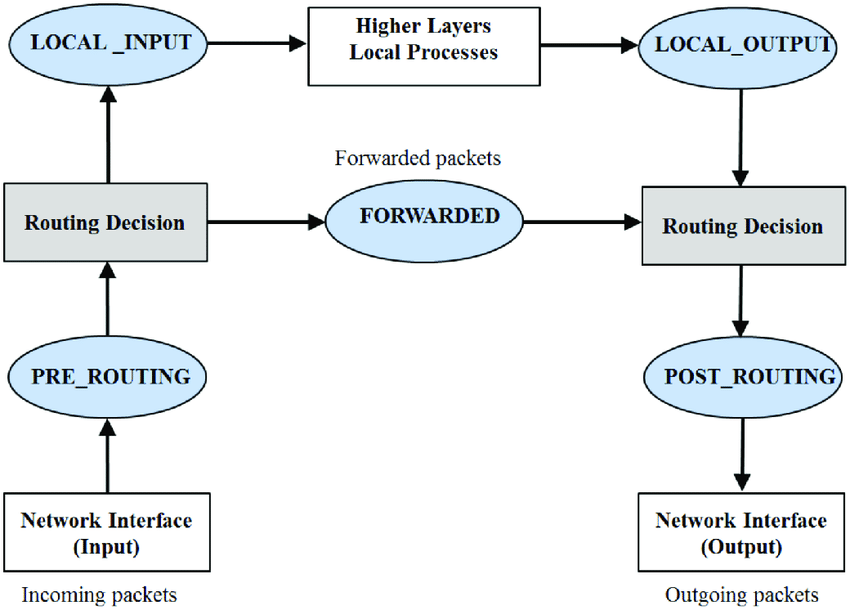
\includegraphics[width=8cm]{netfilter_hooks.png}
    \caption{Flusso del pacchetto attraverso il Linux network stack con Netfilter hook \cite{NetfilterHooks}.}
    \label{fig:netfilter_hooks}
\end{figure}
I moduli Kernel registrati in questo modo, possono assegnare un numero di priorità per identificare deterministicamente in quale ordine verranno eseguite le funzioni di callback.

Quando una funzione di callback viene eseguita, il modulo può decidere di alterare il pacchetto responsabile dell'esecuzione della funzione. Al termine dell'esecuzione, inoltra al framework la propria decisione sul futuro del pacchetto. Il pacchetto può quindi essere scartato, ignorato, inserito in coda per poter essere maneggiato da software che appartengono allo \textit{spazio utente}\footnote{Netfilter è un framework che esegue a livello di Kernel  in Kernel mode e quindi l'utente che esegue software in user mode non potrebbe interagire direttamente con questo.}, o potrebbe proseguire il suo corso attraverso lo stack.

Per interagire con il framework Netfilter dunque è necessario sviluppare un modulo Kernel che possa registrare funzioni di callback presso gli hook o scrivere un applicativo che interagisca con la coda nello spazio utente (user mode).

Per semplificare il processo e non dover specificatamente scrivere un software per  filtrare  i pacchetti spesso si usano programmi come Iptables e Nftables. Attraverso questi software è possibile definire insiemi di regole di filtraggio dei pacchetti.

\subsection{Iptables}
\label{iptables}
Iptables usa tabelle per organizzare queste regole. Nello specifico le tabelle \textit{built-in} di Iptables sono:
\begin{description}
    \item[Filter table] Per controllare il flusso dei pacchetti che entra ed esce dal sistema;
    \item[NAT table] Per ridirigere connessioni verso altre interfacce di rete;
    \item[Mangle table] Per modificare header di pacchetti;
    \item[Raw table] Provvede meccanismo per marcare pacchetti ed escluderli dal tracking di connessione\footnote{Netfilter  riesce a identificare un pacchetto come parte di una connessione e Iptables quindi sfrutta questa capacità in automatico.};
    \item[Security table] Usata per interagire con SELinux\footnote{Security Enhanced Linux è un modulo di sicurezza del Kernel Linux che fornisce insieme di strumenti di sicurezza.}.
\end{description}
Ogni tabella è a sua volta organizzata in \textit{chain} che contengono le vere e proprie regole. Mentre le tabelle rappresentano lo scopo generale delle regole che contengono, le chain rappresentano i Netfilter hook a cui si riferiscono e da cui vengono attivati. Le chain quindi determinano quando le regole al loro interno verranno valutate.
I nomi delle chain fanno riferimento ai nomi degli hook a cui sono associati e sono:
\begin{itemize}
    \item Prerouting;
    \item Input;
    \item Forward;
    \item Output;
    \item Postrouting.
\end{itemize}

Dato che alcune operazioni/decisioni hanno senso solo in alcuni punti del network stack, non ogni tabella ha tutte le precedenti chain registrate presso i rispettivi Netfilter hook. Ad esempio la Filter table hanno solo le Input, Output e Forward chain registrate.

Come detto le regole sono posizionate all'interno delle chain delle tabelle specifiche. Quando una chain è chiamata dal rispettivo hook, i dettagli del pacchetto vengono comparati con le regole con ordine. Ogni regola è divisa in due parti.
La prima parte è quella interessata dei criteri di match con le informazioni del pacchetto. Tra i criteri di match ci sono il protocollo usato, la sorgente, la destinazione, lo  stato della connessione, le porte utilizzate, e molto altro.
La seconda parte invece detta \textit{target} specifica un azione da compiere sul pacchetto. Tra i target più comuni ci sono Accept, Reject, Drop e Jump.

Oltre alle chain built-in è anche possibile creare chain personalizzate. Queste non sono associate ad   hook Netfilter e sono raggiungibili solo attraverso il target Jump, ovvero saltando da una chain built-in a questa. Quando un pacchetto esegue il match con una regola avente target Jump, il controllo può saltare all'interno di chain definite dall'utente. In caso  non vi sia match all'interno di queste, il controllo tornerebbe alla chain d'origine. In questo modo è possibile aumentare l'organizzazione del sistema. 

\subsection{Nftables}
\label{nftables}
Nftables \cite{nftables} è il successore di Iptables, basato anch'esso sul framework Netfilter. Risulta più flessibile, scalabile ed efficiente nel classificare i pacchetti.
La struttura è uguale a quella di Iptables, ovvero è composto di table, che contengono chain, che a loro volta contengono regole.
Tra i vantaggi che offre rispetto a Iptables ci sono:
\begin{itemize}
    \item Una singola regola può avere più target mentre Iptables può averne solo uno per regola;
    \item Possibilità di creare regole più complesse attraverso strutture dati come map, set, concatenazioni, diminuendo quindi il numero di regole da controllare e quindi aumentando l'efficienza;
    \item Non ha table e chain predefinite, sfrutta combinazione di parametri selezionabili come il tipo di hook e lo scopo per determinarne il comportamento;
    \item Più facile da configurare;
    \item Possibilità di gestire regole IPv4 e IPv6   attraverso lo stesso tool, mentre in Iptables le configurazioni sono gestite separatamente\footnote{viene usato  tool \textit{iptables} per le configurazioni IPv4 e \textit{ip6tables} per quelle IPv6.}.
\end{itemize}

\subsection{Firewalld}
\label{firewalld}
Firewalld \cite{firewalld} è uno strumento di gestione del Firewall che sfrutta  Nftables o Iptables. È il tool di gestione Firewall predefinito di RHEL 7, CentOS, Fedora e altre distribuzioni Linux. Esso agisce come  un'interfaccia front-end e non è quindi un Firewall \textit{stand-alone}.
Firewalld è strutturato in zone. Le interfacce di rete o range di indirizzi IP possono  essere assegnati a zone specifiche. Una zona  dichiara quali porte o servizi sono permessi o bloccati, oltre a poter definire ulteriori regole più complesse. Le zone sono formulate come file XML e sono posizionate all'interno della directory di Firewalld.
Il funzionamento alla base di Firewalld è indipendente dal fatto che venga utilizzato Nftables o Iptables. Al boot esegue uno script Python che converte e carica le regole, configurate con Firewalld, in Nftables o Iptables. Sono anche disponibili interfacce grafiche che ne semplificano ulteriormente l'utilizzo.

\section{Docker}
\label{docker}
In uno scenario di normale sviluppo di un'applicazione \textit{end-to-end}, dove si vogliono utilizzare diversi servizi che devono cooperare tra loro, ci possono essere le seguenti problematiche da tenere in considerazione:
\begin{description}
    \item[Compatibilità/dipendenze] I diversi servizi dell'applicativo possono richiedere differenti versioni della stessa libreria. Le librerie devono essere compatibili con il sistema operativo e l'hardware sottostante. Inoltre queste hanno dipendenze che devono essere soddisfatte.
    Il problema di soddisfare tutte queste esigenze contemporaneamente per permettere il corretto funzionamento dell'applicativo è conosciuto come \textit{Matrix~from~hell};
    \item[Tempi di Setup] La configurazione di un nuovo ambiente di sviluppo da zero sottintende che lo sviluppatore debba assicurarsi di avere il giusto sistema operativo e le librerie necessarie nelle versioni corrette, e che le dipendenze siano risolte correttamente. Questo processo può essere laborioso e non banale,  oltre che richiedere una considerevole quantità di tempo;
    \item[Differenti ambienti di sviluppo] Essendoci diversi ambienti di sviluppo, test e produzione, non è detto che, una volta completata una modifica,  l'applicativo funzioni correttamente quando viene eseguito in un ambiente differente.
\end{description}

Questi sono alcuni dei motivi per cui può essere utile containerizzazione i servizi.
Con containerizzazione si intende raggruppare  il codice software e tutti i relativi componenti necessari, come librerie, framework e altre dipendenze, in modo che risultino isolate in un proprio contenitore, detto \textit{Container}.

In questo modo è possibile eseguire e spostare il software o l'applicazione contenuta all'interno in qualsiasi ambiente o infrastruttura indipendentemente dal sistema operativo eseguito.
Lo scopo quindi della containerizzazione è il poter eseguire applicativi, servizi, processi ovunque, in qualsiasi momento e in un ambiente isolato, risolvendo in questo modo le problematiche sopra citate.

Un Container può essere visto come un processo che dà all'utente l'illusione di eseguire sopra un sistema operativo, si parla infatti di \textit{lightweight process virtualization}. In particolare sfruttano componenti del Kernel Linux per virtualizzare, isolare e gestire le risorse.

I Container condividono il Kernel del sistema operativo sul quale eseguono, così facendo non hanno bisogno di dover virtualizzare il sistema operativo per poter eseguire componenti software \cite{mouat2015using}.  
Essi \textit{vivono} solo per il tempo dell'esecuzione del processo o del servizio che ospitano.
Per questi motivi dunque sono  più leggeri e  meno dispendiosi in termini di potenza di calcolo di una macchina virtuale, oltre a risultare più veloci in termini di \textit{boot} e \textit{shutdown}.

Dato che i Container sono soluzioni a basso livello solitamente difficili da utilizzare, si usano soluzioni software come Docker  \cite{docker}  che sfruttano le capacità del Kernel Linux per crearli e gestirli.

Docker usa le Docker Image, che rappresentano una serie di istruzioni da eseguire sequenzialmente, al fine di creare un Docker Container \cite{mouat2015using}. Contengono inoltre il codice, le librerie necessarie, tool, dipendenze e tutto quello che è indispensabile per eseguire l'applicativo o il servizio contenuto. Quando viene eseguita una Docker Image, si creano una o più istanze di Container, usando quell'immagine come template.


Le Docker Image vengono create a partire da file di configurazione, detti Dockerfile. Nel Dockerfile viene specificata la Docker Image di partenza e tutte le operazioni, che su questa verranno eseguite, atte a costruire il template per i futuri Container. Quando viene eseguita la \textit{build} dell'immagine, ogni operazione all'interno del Dockerfile costituisce un livello che viene posta sopra al livello dell'operazione precedente. Ogni livello contiene solo le differenze dal livello precedente. In questo modo se la build dovesse fallire, al tentativo successivo riprenderebbe dal livello in cui si era interrotto. Questo meccanismo permette anche di accelerare i tempi in caso di \textit{rebuild} in seguito a piccoli cambiamenti nel Dockerfile, in quanto i livelli verranno ricostruiti dal primo cambiamento a seguire.

I livelli sono \textit{read only} e sono condivisi tra tutte le istanze di Container della stessa immagine. Quando viene eseguito un Container, si crea un ulteriore livello che è \textit{readable} e \textit{writeable}, che chiameremo 'livello container'. Quando viene modificato un file read only all'interno di un  livello non modificabile, si crea una copia locale di quel file nel livello container e la modifica viene eseguita sulla  copia\footnote{tecnica definita come \textit{Copy on write}.}.

Quando si crea un nuovo file questo viene aggiunto  al livello container. Nel momento in cui il Container viene rimosso o finisce la propria esecuzione, tutto il contenuto del livello container viene cancellato. Se è richiesta  persistenza di alcune directory  e del relativo contenuto è necessario eseguire il \textit{mount} di una directory dell'host all'interno del container con direttive apposite.  Questo equivale a livello logico all'associare una directory dell'host a una directory del Container, così che al termine dell'esecuzione i dati all'interno della directory del Container persistano nella directory dell'host.

A livello di rete, Docker, crea di default tre network a cui i Container possono essere associati:
\begin{description}
    \item[Bridge] Rete interna privata, solitamente con indirizzo 172.17.0.0/16. Se non viene specificato diversamente un Container viene associato a questo network di default;
    \item[None] Un Container associato a questa tipologia di rete non potrà comunicare con nessun altro Container;
    \item[Host] Il Container viene associato direttamente a rete di host.
\end{description}

I Container possono comunicare tra loro se sono associati alla stessa rete, permettendo quindi di creare applicativi complessi in cui più servizi comunicano tra loro.
Entrando nel dettaglio, Docker usa i \textit{namespace} per creare copie dello stack di rete della macchina host  e interfacce \textit{Veth} per permettere a coppie di Container di comunicare tra loro.

Se un Container è associato a una rete interna, può essere raggiunto dal network dell'host che lo ospita attraverso un'operazione di \textit{port mapping}. In questo modo si può associare una porta del Container a una porta dell'host, quindi un pacchetto che fluisce attraverso la porta specifica dell'host verrà consegnato in automatico alla porta specifica del Container.



Docker può prelevare le immagini da repository di immagini Docker detti Registry, che possono contenere anche centinaia di migliaia di immagini di applicazioni e servizi pronti per essere scaricati ed eseguiti in Container.

Per sviluppare applicazioni complesse  potrebbe essere necessario eseguire molteplici Container contemporaneamente. Per evitare di dover eseguire manualmente ogni container, esistono tool di orchestrazione dei Container. Un esempio di questo genere di tool è \textit{Docker Compose}, che permette grazie a un unico file di configurazione in formato YAML di eseguire contemporaneamente  molteplici Container.
\clearpage
\chapter{Intrusion Detection System (IDS)}
\label{IDS}
Un Intrusion Detection System è un software o hardware che identifica azioni non legittime su computer, col fine di preservare la sicurezza del sistema. In particolare ha l'obiettivo di identificare traffico di rete e uso di computer non legittimi, che non potrebbero essere identificati da un normale Firewall. Si possono identificare principalmente due tipi di IDS \cite{khraisat2019survey}:
\begin{itemize}
    \item Signature-based IDS (SIDS);
    \item Anomaly-based Intrusion Detection System (AIDS).
\end{itemize}

Con SIDS si intende strumenti di rilevazione basati su tecniche di \textit{pattern matching} per scovare attacchi già noti. Quando la \textit{signature}\footnote{attraverso l'estrazione di \textit{feature} prefissate si può generare la firma  di un particolare evento per usarla come identificativo univoco di questo.} di un evento combacia con la signature di un'intrusione nota all'interno del database di signature, viene generato un segnale d'allarme.

Questi solitamente hanno un'ottima accuratezza per quanto riguarda la rilevazione di minacce già note ma non possono rilevare \textit{attacchi zero-day}\footnote{attacchi informatici che sfruttano vulnerabilità di cui non si conosce l'esistenza o che non sono state ancora risolte.} dato che non esistono signature di tale attacco sino a quanto la signature di questo viene estratto e aggiunto al database.
Gli approcci SIDS soffrono anche nell'identificare le varianti di malware noti, in quanto variazioni nel codice potrebbero comportare una signature differente al malware originale.

Approcci tradizionali di SIDS sfruttano i \textit{log} di macchina host e l'analisi del traffico di rete per scovare azioni, comandi, pattern riconducibili a malware noti.


L'approccio Anomaly-based parte dal presupposto che il comportamento non legittimo differisca da quello legittimo.
Viene creato il modello di comportamento del sistema. Le tecniche usate per effettuare appartengono alle seguenti categorie:
\begin{itemize}
    \item Machine Learning;
    \item Statistical-based;
    \item Knowledge-based.
\end{itemize}
Il modello viene creato in una prima fase di \textit{training} in cui viene osservato il normale comportamento del sistema. Segue una fase di \textit{testing} in cui si usa un nuovo data set per stabilire l'accuratezza del sistema nel rilevare intrusioni. 
Ogni significativa deviazione del comportamento osservato dal modello è considerata un'anomalia e trattata come un'intrusione.

Il vantaggio primario di questo approccio è la capacità di rilevare attacchi zero-day dato che è basato sul comportamento e non sulle signature.


Un'altra classificazione possibile degli IDS è basata sul tipo di sergenti dati che utilizzato per le rilevazioni.  In particolare si parla di:
\begin{itemize}
    \item Host-Based IDS (HIDS);
    \item Network-Based IDS (NIDS).
\end{itemize}

Gli HIDS analizzano i log originati dal sistema host e dalle \textit{sorgenti di Auditing}\footnote{sorgenti di eventi generati in seguito a controlli specifici.}. Sono capaci di individuare minacce che non usano traffico di rete.

I NIDS monitorano il traffico di rete estratto attraverso appositi strumenti di cattura. Possono essere usati per monitorare molteplici computer su stessa rete al contrario di HIDS che sono installati su una macchina specifica. Sono capaci di individuare minacce esterne prima che si propaghino tra dispositivi. A seconda della rete da monitorare possono essere richieste capacità di hardware elevate per gestire correttamente alti traffici di rete.


Il giusto deploy di molteplici NIDS in determinati punti strategici della rete in combinazione con HIDS e Firewall possono provvedere a una  protezione robusta sia ad attacchi esterni che interni.

Di seguito verranno analizzati i due NIDS utilizzati ma prima è necessaria una piccola premessa sulla duplicazione del traffico di rete, operazione necessaria per poter analizzare una copia dei dati che fluiscono attraverso la rete.
\section{Duplicazione del traffico di rete}
La duplicazione del traffico di rete può avvenire in due modi \cite{svoboda2015network}:
\begin{itemize}
    \item Inline;
    \item Mirroring.
\end{itemize}
Con mirroring si intende utilizzare le capacità built-in degli switch o router, mentre con inline si intende utilizzare un dispositivo apposito di duplicazione del traffico lungo la linea di rete.

\subsection{Port Mirroring}
Il port mirroring è una funzionalità spesso già integrata nei router e switch a livello enterprise. Il traffico che passa attraverso una porta dello switch o router viene 'specchiato' verso un'altra porta. La porta selezionata per eseguire l'output della copia del traffico è detta Switch Port Analyzer (SPAN) o \textit{mirror port}. Dato che il compito primario di switch o router è il forwarding dei pacchetti, la copia dei dati è data con bassa priorità. Questo può portare a drop di pacchetti anche quando vi è basso volume di traffico. 
Va considerato inoltre che queste porte utilizzano slot sullo switch o router che potrebbero altrimenti venir utilizzati per gli scopi di forwarding.

Il port mirroring attraverso lo SPAN può anche causare effetti negativi sullo switch, intaccando quindi il traffico di rete. In caso di misconfigurazioni inoltre potrebbe intaccare anche la performance del network.

Usa una singola porta di uscita per aggregare più link e i relativi canali di up-link e down-link. Così facendo è molto probabile che la linea di output si saturi portando a perdita dei pacchetti.

Usato solitamente per monitorare bassi volumi di dati in luoghi in cui non è presente un Test Access Port. 
Rimane comunque l'unico mono per monitorare certe specie di dati come quelli che navigano port-to-port in stesso switch.



\subsection{Test Access Port}
Il Test Access Port (TAP) è un device di cattura del traffico di rete posizionato lungo la linea cablata. Attraverso a uno splitter interno è capace di copiare i dati e reindirizzarli verso porte di uscita.

Separa canali di up-link e down-link diminuendo  la possibilità di drop di pacchetti.
Il TAP è in grado quindi di creare una copia esatta del flusso bidirezionale a pieno rate di linea, che ne consegue nella piena fedeltà di monitoraggio.
Ci sono TAP passivi e attivi.
Quelli passivi non sono alimentati a  corrente e quindi in caso di malfunzionamenti della linea elettrica il sistema può comunque funzionare correttamente. Tuttavia i TAP passivi in rame distorcono il segnale rendendoli inadoperabili per linee sopra un gigabit al secondo. Esistono TAP passivi ottici per ovviare al problema, al costo di un indebolimento del segnale ottico sulla linea.
Quelli attivi sono alimentati da corrente elettrica e ritrasmettono e duplicano il segnale senza introdurre distorsioni.

I TAP passivi non richiedono configurazioni o interventi particolari, offrendo continuo accesso ai dati.


\subsection{Port mirroring via software}
Altri approcci meno scalabili sono possibili, come ad esempio l'utilizzo di software e tool per eseguire la copia e l'inoltro del traffico di rete.
In questo caso è stato usato Iptables per fare test di port mirroring via software, utilizzando la seguente regola:
\begin{verbatim}
    iptables -t mangle -I PREROUTING -j TEE --gateway 100.0.0.2 
\end{verbatim}
Questo comando aggiunge una regola all'inizio della chain di \textit{Prerouting} nella tabella \textit{Mangle} in cui specifica di inviare una copia del pacchetto al nodo di rete specificato.



\section{Security Onion}
Security Onion \cite{secOnion} è   una  piattaforma gratuita e open source per Network Security Monitoring (NSM) ed Enterprise Security Monitoring (ESM) \cite{secOnionDoc}.
Con  ESM si intende l'aggiunta delle capacità di  monitoring degli \textit{end-point} alla soluzione NSM.
\begin{figure}[hbtp]
    \centering
    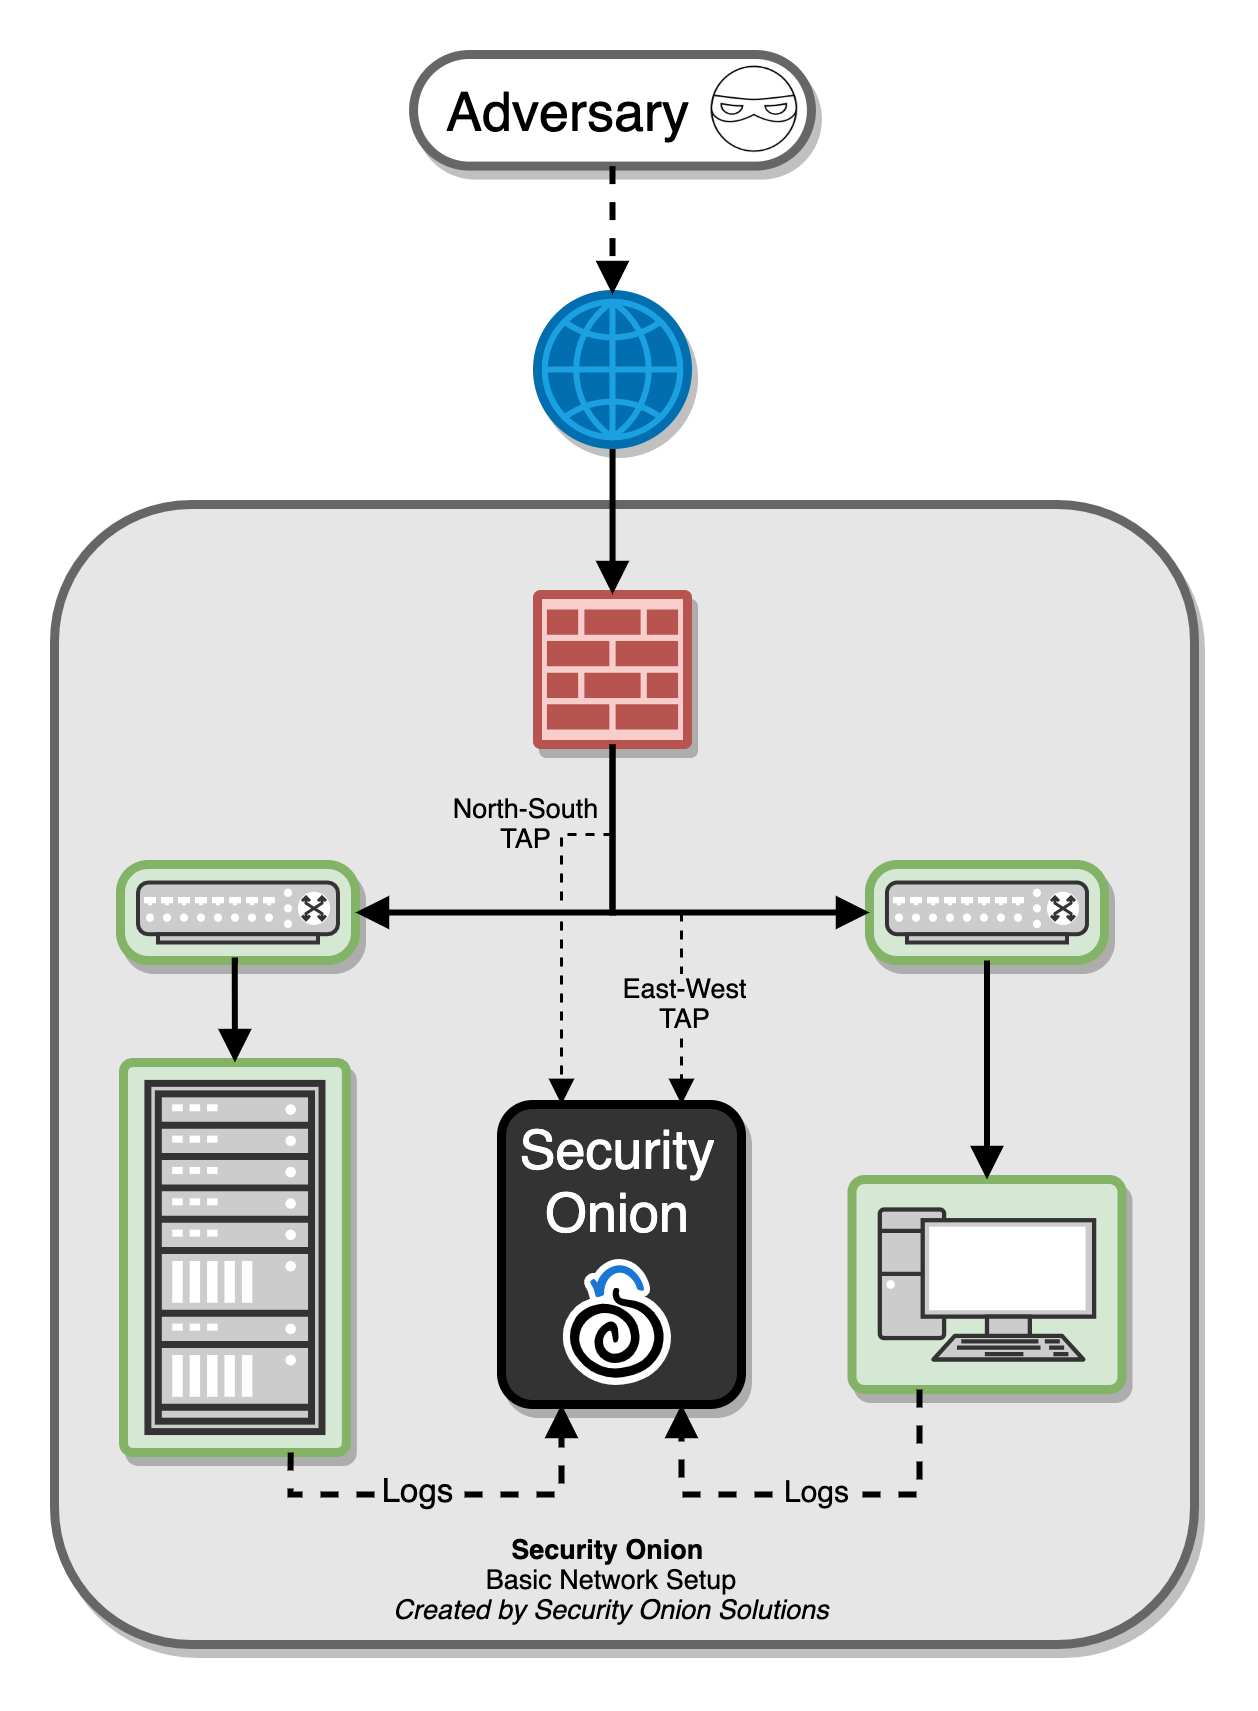
\includegraphics[width=8cm]{res/fig/SecOnionExample1.png}
    \caption{Esempio di utilizzo di Security Onion all'interno di un network enterprise \cite{SecOnionFig1}.}
    \label{fig:seconionexample}
\end{figure}

Nella figura \ref{fig:seconionexample} si può vedere un esempio di utilizzo di Security Onion all'interno di un network enterprise.
In questo caso il traffico di rete viene duplicato e inviato attraverso porte TAP a Security Onion che ne esegue l'analisi. Nel mentre anche i log dei sistemi monitorati vengono raccolti e analizzati. In questo modo si hanno funzioni di NIDS e di HIDS.

Di seguito verranno brevemente descritti i principali software che vengono utilizzati all'interno di Security Onion per poi analizzare l'architettura distribuita di tale IDS e il suo deploy all'interno dell'infrastruttura di testing.

\subsection{Tool integrati}
Di seguito verranno descritti i principali tool utilizzati da Security Onion durante il funzionamento all'interno di un'architettura distribuita. L'architettura in questione verrà meglio analizzata successivamente.
\subsubsection*{Suricata}
Suricata \cite{suricata} è un NIDS open source, maturo e robusto. Ispeziona il traffico di rete usando regole e linguaggio di signature oltre ad avere supporto a LUA \cite{LUA} scripting per rilevazione di minacce complesse. Attraverso l'integrazione di linguaggio di scripting è possibile, ad esempio, elaborare il payload di un pacchetto di rete prima di cercare possibili fingerprint match, aumentando le difese contro le tecniche di offuscamento. 
Suricata è anche in grado di agire attivamente in caso di intrusione, per questo motivo è anche classificato come Intrusion Prevention System (IPS). Inoltre è anche in grado di memorizzare PCAP file\footnote{file contenenti pacchetti catturati dal traffico di rete.} per analisi successive.
Viene quindi principalmente usato come SIDS all'interno di Security Onion.
\subsubsection*{ZEEK}
ZEEK \cite{ZEEK} è un tool di analisi del traffico di rete. Al contrario di Suricata non è ottimizzato per la ricerca di signature e non fornisce memorizzazione della cattura del traffico di rete. Il suo scopo è interpretare il traffico di rete e generare notevoli volumi di informazioni riguardanti il comportamento della rete, fornendo visibilità e contesto, oltre a offrire capacità come:
\begin{itemize}
    \item Analisi della performance di rete;
    \item Profiling di host e servizi;
    \item Anomaly detection.
\end{itemize}
In Security Onion viene affiancato a Suricata per la rilevazione di minacce attraverso l'analisi del traffico di rete. Mentre Suricata permette di identificare attacchi basandosi sul signature matching, ZEEK permette di reperire il contesto dell'attacco,  offrendo tutti i metadata necessari per analizzare al meglio la situazione e poter quindi agire di conseguenza.

\subsubsection*{Stenographer}
Stenographer \cite{stenographer} è un utility per la cattura del traffico di rete cui scopo è memorizzare tutto il traffico catturato su disco per scopi di intrusion detection e incident response.
Fornisce un'implementazione ad alta performance della scrittura dei pacchetti da NIC a disco e gestisce la cancellazione automatica quando la memoria si satura. 
Offre inoltre metodi per la lettura rapida ed efficiente di set specifici di pacchetti oltre a un linguaggio di query.

Si può accedere a cattura dei pacchetti memorizzai attraverso una qualsiasi interfaccia PCAP o attraverso Command Line Interface (CLI).

\subsubsection*{Strelka}
Strelka \cite{strelka} è un sistema di scansione di file in tempo reale, utilizzato per la ricerca e rilevazione di minacce o per analisi di incident response. Il suo scopo è l'estrazione di file e metadati su larga scala. È in grado di utilizzare regole YARA\footnote{le regole YARA usano pattern  come sequenze  di byte  o stringhe riconducibili  a malware noti.} per l'identificazione di minacce note.

In Security Onion viene utilizzato per analizzare i file estratti da ZEEK e Suricata durante l'analisi del traffico di rete.

\subsubsection*{Sensoroni}
Sensoroni \cite{sensoroni} è un sistema software per il monitoraggio e l'interrogazione di server o dispositivi remoti.
È composto da un server e uno o più agenti.
Gli agenti sono  eseguiti sui dispositivi remoti (sensori) ed eseguono i \textit{job} che sono stati impartiti e accodati dal server. 
Il server offre un'interfaccia utente per gli amministratori per eseguire task come il monitoraggio dei sensori e la gestione dei job.

\subsubsection*{Elastic Stack}
Con Elastic Stack \cite{elasticstack} si intende una collezione di software open source appartenenti alla compagnia Elastic.
Il suo scopo è aiutare l'utente a raccogliere dati da qualsiasi sorgente e in qualsiasi formato per poter poi eseguire ricerche, analisi e visualizzazioni dei dati.
Questa collezione era precedentemente chiamata come ELK stack, dove ELK rappresenta l'acronimo delle sue componenti software, ovvero:
\begin{description}
    \item [Elasticsearch] Motore di ricerca e analisi distribuito, basato su interfaccia RESTful e usato per moltissimi casi d'uso. Componente che rappresenta il cuore dell'Elastic Stack. Mantiene e indicizza i  dati per ricerche veloci e precise.
    In Security Onion riceve i log e ne effettua il parsing prima di memorizzarli e indicizzarli;
    \item [Logstash] Motore di data processing server-side basato su pipeline, capace di raccogliere dati da moltitudine di sorgenti, trasformali e inoltrarli.
    In Security Onion trasporta i log, su cui non è ancora stato effettuato parsing,  a Elastic Search;
    \item [Kibana] Interfaccia GUI  che permette di visualizzare i dati memorizzati in Elastic Search e di navigare l'Elastic Stack. Permette di visualizzare in tempo reale flussi di dati di notevoli dimensioni e di aumentarne la comprensione attraverso grafici;
\end{description}

L'ELK stack si evolse nell'Elastic Stack in seguito all'aggiunta di Beats alla collezione.
I Beats sono installati come agenti su dispositivi remoti e vengono utilizzati per inviare dati di diversa natura (log, metriche, dati di rete, etc.) direttamente a Elastic Search  o indirettamente attraverso Logstash. Security Onion in particolare usa FileBeat per inoltrare log a Elastic Search.

Lo stack viene principalmente usato per la gestione di ingenti quantità di dati o in caso siano necessarie capacità di ricerca avanzate sui dati. In Security Onion viene utilizzato per inoltrare, ricevere, memorizzare, indicizzare, visualizzare e analizzare i vari log generati.

\subsubsection*{ElastAlert}
ElastAlert \cite{elastalert} è un framework per l'allerta su anomalie, picchi  o altri pattern di interesse all'interno dei dati custoditi in Elasticsearch. Interroga Elasticsearch e fornisce un meccanismo di allerta in tempo reale con molteplici tipi di output. 

\subsubsection*{Curator}
Curator \cite{curator} è un Utility utilizzata all'interno di Elastic Stack per la gestione degli indici di Elasticsearch. In particolare: 
\begin{enumerate}
    \item Ottiene lista di indici da cluster, che verrà chiamata \textit{actionable};
    \item Itera su lista di filtri definiti da utente per rimuovere progressivamente indici dalla lista actionable;
    \item Esegue diverse azioni su elementi rimasti a seguito del filtraggio.
\end{enumerate}

\subsubsection*{Redis}
Redis \cite{redis} è uno store di strutture dati in memoria open source, utilizzato come database, cache e message broker. Supporta strutture dati come stringhe, hash, liste, insiemi, insiemi ordinati, etc.
I  dataset vengono mantenuti in memoria principale rendendo l'accesso estremamente veloce, ma i dati possono anche essere resi persistenti all'occorrenza.

Security Onion utilizza Redis come contenitore temporaneo dei log ricevuti da Logstash. I log così memorizzati vengono poi reperiti da Logstash e consegnati a Elastic Search.

\subsubsection*{Security Onion Console (SOC)}
SOC è l'interfaccia web attraverso cui un'analista può accedere ai vari tool di analisi offerti dalla piattaforma.
L'interfaccia web è divisa più sezioni.
Tra le sezioni built-in vi sono:
\begin{description}
    \item[Alerts] Visualizza gli \textit{alert} che Security Onion sta generando. È possibile visualizzarne i dettagli e i PCAP a cui sono associati o aggiungere l'alert a dei Case;
    \item[Dashboard] Permette di avere un overview generale del sistema. Personalizzabile all'occorrenza;
    \item[Hunt] Simile alla Dashboard ma più mirata alla ricerca di minacce;
    \item[Case] Interfaccia per gestire i Case. Attraverso i Case è possibile raggruppare più alert che si ritengono essere associati per studiare nel dettaglio la possibile intrusione o anomalia;
    \item[PCAP] Permette di analizzare i PCAP raccolti con Stenographer, anche in relazione a un particolare evento;
    \item[Grid] Permette di controllare lo status dei nodi appartenenti al sistema Security Onion.
\end{description}

Oltre alle sezioni elencate vi sono collegamenti a tool che hanno interfacce web separate come Kibana, tra cui:
\begin{description}
    \item [Grafana ]  Permette di visualizzare attraverso grafici lo status e informazioni vitali del sistema come l'uso della CPU, RAM, traffico di rete, etc. \cite{grafana};
    \item [Playbook] Consente di creare una lista di strategie di rilevazione, dette \textit{Play}. Ogni Play è composto di obiettivo, configurazione e \textit{follow-up}. L'obiettivo è l'oggetto da rilevare (eg. un'anomalia, un'intrusione) e necessita della configurazione necessaria per poter essere rilevato. Nel caso di Security Onion le configurazioni sono basate su ElastAlert. Con follow-up si intende le azioni da eseguire per validare e/o correggere quanto accaduto. 

    I risultati delle Play sono disponibili nelle sezioni Haunt, Dashboard e Kibana. Quando il risultato di una Play è di gravità elevata viene anche generato un alert visualizzabile nell'apposita sezione.
    Quando una Play viene attivata, la configurazione ElastAlert viene inserita in produzione;
    \item [ATT\&CK Navigator ] Il Navigator ATT\&CK è progettato per fornire una navigazione e un'annotazione di base delle tecniche appartenenti alla \textit{matrice MITRE ATT\&CK}\footnote{matrice standardizzata di tattiche e tecniche di minacce informatiche.} \cite{att&ck}. Può essere utilizzato  per visualizzare la  copertura difensiva, la pianificazione del  team di attacco/difesa, la frequenza delle tecniche rilevate e molto altro.
    Inoltre si integra con Playbook, permettendo di visualizzare le Play in relazione alle tecniche coperte nella matrice ATT\&CK per avere un'idea ancora più chiara della copertura difensiva \cite{att&ckNavigator}.
\end{description}

\subsubsection*{Host-based visibility tools}
Security Onion permette anche la raccolta di molti tipi di log generati dagli host che si desiderano monitorare. L'host può scegliere tra diverse tecnologie agent-based per effettuare diversi task di controllo sull'host e inviare i relativi log a Security Onion.

Attraverso specifiche tecnologie installate sugli host da monitorare e l'analisi dei relativi log è possibile implementare il lato HIDS di Security Onion già accennato in precedenza.
In alternativa, si potrebbe decidere di inviare log arbitrari usando una delle seguenti tecnologie:
\begin{description}
    \item[Osquery] Osquery \cite{osquery} è un agent  capace di astrarre l'host, sul quale è installato, a database relazionale. L'agent può quindi essere interrogato usando sintassi SQL per avere informazioni sul sistema. Questo può anche essere usato inviare i log a Security Onion;
    \item[Wazuh] Wazuh \cite{wazuh} è un agent con capacità di HIDS. Verrà approfondito meglio nella sezione inerente gli agent. Permette anche l'inoltro di log a Security Onion;
    \item[FileBeat] Come già spiegato precedentemente, FileBeat \cite{filebeat} è in grado di fornire trasporto di log dedicato;
    \item [Syslog] Syslog \cite{syslog} è un protocollo di rete usato per l'invio di log semplici. Utile nel caso non sia possibile installare un agent sull'end-point.
\end{description}

\subsection{Architettura}
Security Onion dispone di diverse Architetture possibili per adattarsi alle diverse esigenze e risorse, tuttavia l'architettura raccomandata è quella distribuita che verrà di seguito analizzata.

L'architettura distribuita offre maggior scalabilità e una maggior performance in quanto basta aggiungere nodi per poter maneggiare più traffico di rete o sorgenti di log.

Si compone di  tre tipologie di nodi:
\begin{itemize}
    \item Forward Node;
    \item Manager Node;
    \item Search Node.
\end{itemize}

\vspace{5mm}
Il Forward Node è un sensore che esegue Zeek, Suricata, Stenographer e Wazuh per generare log. In particolare, come detto, Zeek e Suricata analizzano il traffico di rete, Wazuh funge da HIDS sull'end-point e Stenographer memorizza i PCAP all'interno di esso. Tutti i log vengono inviati attraverso FileBeat a Manager Node. I PCAP vengono all'occorrenza reperiti dal Forward Node attraverso il Sensoroni agent.
Strelka analizza all'occorrenza i file estratti da Zeek.

\vspace{5mm}
Il Manager node riceve attraverso Logstash i log  inviati dai sensori e li mette in coda su Redis.
Hanno anche un'istanza di Elasticsearch che viene usata per memorizzare i Case e le configurazioni centrali oltre a effettuare le query sulle istanze ElasticSearch dei Search Node.
Esegue inoltre:
\begin{itemize}
    \item Security Onion Console per permettere a un'analista di interfacciarsi con esso;
    \item Kibana per visualizzare  i log indicizzati con Elasticsearch;
    \item Curator per gestire gli indici ed eseguire operazioni su essi;
    \item ElastAlert per generare alert  in Elasticsearch;
    \item Wazuh come istanza HIDS locale;
\end{itemize}
Attraverso il Manager Node l'analista può interfacciarsi con Security Onion per eseguire query e reperire/analizzare dati.

\vspace{5mm}
Il Search Node usa Logstash per consumare log da coda in Manager Node per poi eseguirne il parsing e l'indicizzazione con ElasticSearch. Usa Curator per gestire gli indici e ha Wazuh installato come agent HIDS. Quando analista esegue una query su Manager Node, questo esegue a sua volta query su Search Node e ne restituisce il risultato.
L'aggiunta di Search Node può avvenire attraverso \textit{cross cluster search}, dove ogni Search Node è indipendente, o attraverso \textit{clustering} tradizionale in cui tutti i Search Node si uniscono logicamente per formare un singolo cluster.

\subsection{Deploy e requisiti Hardware}
In questa sezione verrà inizialmente descritto in che modo i vari nodi dell'infrastruttura utilizzano le risorse di calcolo, per poi passare all'elenco dei requisiti minimi di sistema \cite{securityOnionRequirements} dei singoli nodi e l'effettivo dispiegamento delle risorse invece utilizzato sulle macchine virtuali.
Le risorse sono state calcolate considerando 1 Gbps come massimo carico di rete.
In conclusione seguirà una breve analisi del  deploy dell'IDS all'interno dell'infrastruttura di testing.


\subsubsection*{Manager Node}
Il Manager Node utilizza la CPU principalmente per ricevere i log in ingresso e posizionarli in coda su Redis, eseguire web server e aggregare i risultati ottenuti dai vari Search Node in seguito a query. 

Le risorse della RAM vengono usate in particolare da esecuzione di Logstash e Redis. Le dimensioni della RAM impattano direttamente sulla dimensione della coda Redis.

La memoria secondaria invece  per utilizzi generali di sistema operativo e per mantenere la Dashboard di Kibana.


\begin{table}[hbtp]
    \centering
    \begin{tabular}{|l|c|c|c|}
        \hline
        & CPU (N. core) & RAM (GB) & DISK (GB) \\
        \hline
        Minimi     & 4-8 & 16 & 200-1000   \\
        \hline
        Utilizzati & 8   & 16  & 200 \\
        \hline
    \end{tabular}
    \caption{Requisiti minimi e risorse effettivamente assegnate al Manager Node.}
    \label{tab:requisitiHw1}
\end{table}


\subsubsection*{Search Node}

I Search Node usano la CPU principalmente per eseguire il parsing e l'indicizzazione dei log, ovviamente la richiesta di CPU aumenta all'aumentare del numero di log da elaborare.

La quantità di RAM a disposizione influenza direttamente la velocità di ricerca all'interno degli indici e l'affidabilità del sistema di ricerca. I Programmi principalmente coinvolti nell'utilizzo della RAM sono Logstash ed Elasticsearch.

La memoria secondaria viene utilizzata per memorizzare metadati indicizzati. All'aumentare dello spazio a disposizione è possibile aumentare i tempi di conservazione dei dati.

\begin{table}[hbtp]
    \centering
    \begin{tabular}{|l|c|c|c|}
        \hline
        & CPU (core) & RAM (GB) & DISK (GB) \\
        \hline
        Minimi     & 4-8 & 16-64 & >200   \\
        \hline
        Utilizzati & 8   & 16  & 200 \\
        \hline
    \end{tabular}
    \caption{Requisiti minimi e risorse effettivamente assegnate al Search Node.}
    \label{tab:requisitiHw2}
\end{table}



\subsubsection*{Forward Node}
La CPU di un Forward Node viene utilizzata per analizzare e memorizzare il traffico di rete. All'aumentare del traffico di rete aumenta il consumo del tempo di CPU necessario per l'analisi dei dati. 

Si stima che un worker Suricata o Zeek possa elaborare 200 Mbps, ciò implica che per gestire 1 Gbps di traffico di rete siano necessari almeno 10 worker e quindi almeno 10 core. A questi vanno aggiunti i core necessari per eseguire altri processi fondamentali come Stenographer, etc.

La RAM impiegata dipende molto dai servizi attivi, dal tipo di traffico monitorato, dal traffico attuale e dall'ammontare di pacchetti scartati che si considera accettabile. Viene principalmente utilizzata per scrivere cache e processare il traffico di rete.

La memoria secondaria dipende da quanti dati si vogliono mantenere memorizzati per analisi future e dal periodo di retention\footnote{specifica dopo quanto tempo i dati verranno cancellati.} ritenuto opportuno.
Se ad esempio si volesse mantenere il traffico di rete di un'intera giornata di monitoraggio, supponendo che il traffico di rete ricevuto abbia una media di 1 Gbps, allora sarebbero necessari circa 11 TB di spazio di archiviazione solo per mantenere i PCAP.

\begin{table}[hbtp]
    \centering
    \begin{tabular}{|l|c|c|c|}
        \hline
        & CPU (N. core) & RAM (GB) & DISK (GB) \\
        \hline
        Minimi     & $\approx 12$ & 16-128 & variabile   \\
        \hline
        Utilizzati & 13   & 64  & 500 \\
        \hline
    \end{tabular}
    \caption{Requisiti minimi e risorse effettivamente assegnate al Forward Node.}
    \label{tab:requisitiHw3}
\end{table}


\vspace{7mm}
\subsubsection*{Deploy}
Il primo passo di deploy dell'IDS all'interno dell'infrastruttura di testing è stato creare una VM all'interno del server ESXi e installarci sopra il Manager Node. Il Manager Node ha un'interfaccia di rete collegata alla Vlan con accesso a Internet.

In seguito è stato installato il Search Node all'interno di un'altra VM. Questa ha una sola interfaccia di rete collegata alla stessa Vlan del Manager Node. Il nodo di ricerca è stato quindi collegato al Manager.

Infine è stata creata un'ulteriore VM in cui è stato installato il Forward Node. Questa ha due interfacce di rete. Una collegata alla stessa rete del Manager Node, mentre l'altra è collegata alla botnet Vlan di cui si vuole monitorare il traffico di rete. In particolare quest'ultima deve essere in modalità promiscua\footnote{in modalità promiscua l'interfaccia di rete lascia passare anche il traffico non rivolto all'interfaccia stessa, verso la cpu.}.
In una situazione normale sarebbe necessario duplicare il traffico di rete attraverso TAP o SPAN e inviarne una copia all'interfaccia del Forward Node per poterlo analizzare, ma in questo caso particolare non è necessario. Infatti grazie al network virtualizzato del server ESXi basta impostare il virtual switch in modalità promiscua e tutto il traffico di rete sarà catturabile.

Una volta terminata l'installazione sono state aggiunte regole al Firewall integrato di Security Onion per poter accedere all'interfaccia web del Manager Node. 
Una volta impostato l'indirizzo di rete da monitorare è stato accertato che i servizi funzionassero correttamente.
In particolare sono state attivate tutte le regole built-in di Suricata e sono stati effettuati dei semplici test di scansione con Nmap\footnote{software utilizzato per eseguire scansioni di rete.} \cite{nmap}  per verifica che le scansioni venissero effettivamente  rilevate.

%sistemare grafica e aggiungere tabelle con requisiti minimi e adoperati per ogni nodo.


\subsection{SALT}


Salt \cite{salt} è il componente principale di Security Onion incaricato del management di tutti gli altri nodi del sistema  IDS.

Salt è un framework per l'automazione cui funzionalità principali sono:
\begin{itemize}
    \item Capacità di gestire configurazioni di nodi da remoto;
    \item Esecuzione di comandi  e prelievo di dati su nodi remoti.
\end{itemize}

Oltre a queste capacità offre comunque tantissime altre funzionalità come Job Management, Job Scheduling, File Server, orchestration, etc.


In particolare la funzionalità di Configuration Management offerta permette di centralizzare le configurazioni di tutti i nodi dell'infrastruttura, oltre ad astrarre l'infrastruttura a un insieme di dati.

Basato su architettura Master-Minions, dove master controlla uno o più minion. Comandi sono generati da master verso gruppo di minion, che eseguono task e ne ritornano i risultati/dati a master.

I messaggi tra Master e Minion avvengono attraverso \textit{ZeroMQ message bus} \cite{zeromq}. La comunicazione tra Master e Minion è criptata, utilizzando crittografia a chiave pubblica per l'autenticazione del Minion e  crittografia a chiave privata per scambio di dati.

Salt è basato su agent installati sui  minion ma è anche possibile gestire i nodi attraverso SSH senza dover installare necessariamente un agent apposito (agentless system).

Il framework è scritto in Python ma il sistema di management delle configurazioni è di fatto language-agnostic, ovvero aperto a qualsiasi tipo di linguaggio.
Di default usa YAML\footnote{linguaggio per serializzazione di dati in maniera comprensibile all'utente, utilizzato spesso per file di configurazione.}   \cite{yaml} e Jinja\footnote{template engine.} \cite{jinja} template per le configurazioni.

Tra le feature offerte da Salt vi sono anche:
\begin{description}
    \item[Fault tollerance]  Minion può connettersi a molteplici master contemporaneamente;
    \item[Configuration Management scalabile] Il Design realizzato permette il management di migliaia di nodi;
    \item[Parallel execution] Comandi eseguibili in parallelo;
    \item[Python API] Interfaccia di programmazione semplice con design modulare ed estendibile.
\end{description}



\subsubsection{Remote execution}
Come accennato Salt usa modello master-client in cui master inoltra comandi a client che provvede a eseguirli.

Entrando nel dettaglio, il Salt Master è un server che esegue un particolare processo chiamato \textit{salt-master}.  Esso inoltra comandi a  server (Salt Minion) registrati presso il master che eseguono processo chiamato \textit{salt-minion}.

Salt può anche essere visto come un modello \textit{publisher-subscriber}. Il Master pubblica \textit{job} che devono essere eseguiti e Minion si iscrivono a questi job.

Quando un Minion termina l'esecuzione di un job, invia dati in risposta al Master. Salt usa due porte in particolare su ogni nodo per le comunicazioni tra master e minion.  Queste porte lavorano in contemporanea per ricevere e inviare dati verso il message bus.
Il Message Bus usa ZeroMQ per creare una topologia di rete asincrona per la comunicazione più veloce possibile.
In particolare usa due canali:
\begin{description}
    \item [Pub Channel] Canale usato da master per inviare job a minion. Basato su paradigma pub/sub;
    \item [Req Channel] Canale usato da minion per inviare dati a master. Usato principalmente per eseguire \textit{fetch} di file e inviare risultati di job.
\end{description}


La sintassi di un comando eseguibile da remoto verso uno  o più minion è della seguente forma:

\begin{center}
\begin{BVerbatim}
salt '<target>' <module>.<function> [arguments]
\end{BVerbatim}
\end{center}
\subsubsection{Configuration Management}
Il Configuration Management è eseguito dichiarando in quale stato dovrebbe essere un minion specifico, questo stato è chiamato Salt State. Questi altro non sono che file YAML, attraverso i quali è possibile eseguire il management dell'infrastruttura.
Un esempio di semplice Salt State:
    \begin{Verbatim}[numbers=left, frame=single, fontsize=\small]
        install_network_packages:
            pkg.installed:
                - pkgs:
                    - rsync
                    - lftp
                    - curl
    \end{Verbatim}
L'esempio  mostra un Salt State usato per installare o mantenere l'installazione di alcuni pacchetti. I file Salt State hanno estensione \textit{.sls}.

Per portare manualmente un minion specifico in questo stato si può usare il comando:
\begin{center}
    \begin{BVerbatim}
salt "<nome minion>" state.apply <Salt State> 
    \end{BVerbatim}
\end{center}

Ovviamente non è pensabile eseguire il precedente comando manualmente per portare ogni minion in un determinato stato, soprattutto per ambienti in cui vi sono migliaia di minion con migliaia di State file. Per questo motivo viene usato il \textit{Top File}.

Il Top File è uno State File usato per  mappare i Salt State ai vari minion. In breve, esso descrive dove determinati Salt State devono essere applicati.
Un esempio di Top File è il seguente:
    \begin{Verbatim}[numbers=left, frame=single, fontsize=\small]
        base:
          '*':
             - common
          'minion1':
              - sample
    \end{Verbatim} 
Questo Top File associa il Salt State \textit{common.sls} a ogni minion e \textit{sample.sls} al minion \textit{minion1}
Attraverso il comando che segue è possibile applicare il Top File a tutti i minion:
\begin{center}
    \begin{BVerbatim}
salt * state.highstate
    \end{BVerbatim}
\end{center}

I Salt State possono essere parametrizzati attraverso l'uso di  \textit{pillar} e meccanismi di template.
I pillar sono file in master che contengono dati che devono essere distribuiti a minion. Questi dati possono essere ad esempio dati sensibili, password, configurazioni, chiavi crittografiche, e molto altro.
I pillar sono associati ai vari Minion con un apposito \textit{Top File} dedicato, in modo analogo a quanto avviene con i Salt State.
Un esempio di pillar contenenti id di utenti:
    \begin{Verbatim}[numbers=left, frame=single, fontsize=\small]
        users:
          thatch: 1000
          shouse: 1001
          utahdave: 1002
          redbeard: 1003
    \end{Verbatim}

I dati dei pillar possono essere referenziati all'interno dei Salt State usando dei template, come ad esempio il seguente Salt State:
    \begin{Verbatim}[numbers=left, frame=single, fontsize=\small]
        
        {{user}}:
          user.present:
            - uid: {{uid}}
        
    \end{Verbatim}
Questo State usa la sintassi di template Jinja per creare una logica più complessa, in particolare prende i dati contenuti all'interno del pillar precedentemente definito per assicurarsi che all'interno del minion, a cui verrà applicato lo State, siano presenti gli user id elencati nel pillar.
%qui spiega benissimo:
%https://docs.saltproject.io/en/latest/topics/development/architecture.html 
%https://docs.saltproject.io/salt/user-guide/en/latest/topics/execution-architecture.html

\subsubsection{Salt in Security Onion}
Come già detto Salt è usato all'interno di Security Onion per il management di tutti i nodi all'interno dell'infrastruttura.

Molte delle opzioni di Security Onion sono configurabili attraverso specifici pillar file.

Modificando i Pillar è possibile cambiare le configurazioni di tool. Tra i tool che è possibile modificare attraverso le impostazioni nei Pillar vi sono: Filebeat, Suricata, Zeek, gestione degli alert, etc.


Oltre al mantenere le configurazioni per i vari software, attraverso Salt è anche possibile eseguire comandi sui nodi e controllarne lo stato, permettendo controllo totale sull'infrastruttura Security Onion.


\section{Ossim}
Ossim \cite{ossim} è un prodotto Security Information and Event Management (SIEM)  open source sviluppato da AT\&T Cybersecurity (in passato denominata AlienVault). Un sistema SIEM colleziona dati attingendo da diverse fonti di log all'interno dell'infrastruttura. 
Attraverso l'analisi dei dati è capace di generare allarmi in caso di eventi sospetti, oltre a poter generare report.
Ossim viene integrato con Open Threat Exchange (OTX), una piattaforma in cui utenti possono scambiarsi informazioni su host maligni.

È in grado di supportare log di diversa natura e da molteplici sorgenti. È anche possibile inoltrare coppia di traffico di rete.

Ossim è costituito di tre elementi:
\begin{description}
    \item [Sensore] Primo device ad avere un contatto con i log. Raccoglie log e informazioni che riceve e lì converte in eventi per poi inviarli a Server;
    \item [Server] Processa eventi ricevuti da sensore ed esegue operazioni come correlazione di eventi, pattern recognition e calcolo del rischio. Inoltre esegue anche controlli sfruttando informazioni di OTX;
    \item [Logger] Nodo sul quale vengono memorizzati i log. Comprime, firma e memorizza informazioni in accordo alle retention policy.
\end{description}

Ossim è incentrato sul concetto di Asset. Un Asset è un qualsiasi elemento dotato di indirizzo IP.
Ogni Asset aggiunto deve passare attraverso i seguenti moduli per poter avere il massimo livello di accuratezza di output da Ossim:
\begin{description}
    \item [Asset Discovery] Modulo che identifica Asset e porte note. Cerca inoltre di mantenere un inventario degli Asset identificati;
    \item [Vulnerability Assessment] Identifica vulnerabilità in Asset attraverso scansioni. Le scansioni possono essere più approfondite attraverso autenticazione;
    \item [Intrusion Detection] Costituito da NIDS, HIDS e File Integrity Monitor (FIM). Utilizza tool come Snort per identificare intrusioni in  traffico di rete in generale e Suricata per intrusioni su traffico web based;
    \item [Behavioral Monitoring] Modulo in cui vengono analizzate le anomalie di rete. Utilizza modulo Netflow per identificare cause di spikes di rete, propagazione di malware, etc.
    Possiede anche capacità di monitoraggio dell'availability di host e servizi;
    \item [Security Intelligence] Modulo in cui processamento/computazione di eventi è eseguito. Tutte le info prese da moduli precedenti vengono analizzate al suo interno per creare report. 
\end{description}

Ossim e l'intera infrastruttura è configurabile e gestibile una volta installato attraverso l'interfaccia web.


\subsection*{Deploy e requisiti Hardware}

Ossim è stato utilizzato come IDS da affiancare a Security Onion. È stato utilizzato principalmente per poter confrontare i risultati di Security Onion con un secondo IDS e per approfondire un sistema  IDS alternativo.

Per semplicità ne è stato eseguito il deploy in formato stand-alone, ovvero con tutti e tre gli elementi che lo compongono in stesso host.

La macchina virtuale sul quale è stato installato OSSIM ha due interfacce di rete:
\begin{itemize}
    \item  NIC di management collegata alla Vlan con accesso a Internet per potersi interfacciare con la web Gui;
    \item  NIC collegata alla botnet Vlan in modalità promiscua, necessaria per sniffare il traffico di rete.
\end{itemize} 

I requisiti Hardware richiesti  e soddisfati per gestire dai 1000 ai 2000  eventi al secondo sono i seguenti:
\begin{table}[hbtp]
    \centering
    \begin{tabular}{|l|c|c|c|}
        \hline
        & CPU (N. core) & RAM (GB) & DISK (GB) \\
        \hline
        Minimi     & 8 & 16-24 & 500-1000   \\
        \hline
        Utilizzati &  8  & 24 & 500 \\
        \hline
    \end{tabular}
    \caption{Requisiti minimi e risorse effettivamente assegnate ad Ossim.}
    \label{tab:requisitiHw4}
\end{table}

\chapter{Studio Botnet 1 - Byob}
%descrizione OK
%funzionamento ad alto livello OK
%funzionamento a basso livello
%deploy (docker), note debug e modifiche
%rilevamento con ids
    

Byob \cite{byob} è una botnet open source scritta in Python, creata appositamente per scopi educativi e di testing.
Si compone di quattro categorie di moduli principali:
\begin{itemize}
    \item Server Module;
    \item Client Module;
    \item Post-exploitation Modules;
    \item Core Modules.
\end{itemize}

I moduli Core racchiudono le funzionalità principali di Byob e sono utilizzate all'interno del client module e del server module.  

Il modulo server viene utilizzato per inizializzare il C\&C server. Utilizza Flask \cite{flask} come framework per le funzionalità di web server e  dispone di un database Sqlite \cite{sqlite} per mantenere i dati e le sessioni dei bot anche a distanza di tempo e in presenza di disconnessioni. Offre controllo sui bot attraverso console collegata via \textit{reverse-shell}\footnote{shell remota a cui viene reindirizzato input e output verso host che vuole accedervi.} o attraverso interfaccia web dedicata. Basato su topologia centralizzata con paradigma push-based (il server invia i comandi ai bot).

Il modulo client è utilizzato per creare i payload che verranno utilizzato per generare i bot. In particolare il payload è un multi-stage installer che verrà analizzato meglio nel dettaglio.  Il bot così generato sarà in grado di importare moduli necessari e arbitrari direttamente dal server e di caricarli in memoria, non lasciando così traccie su disco. Questo meccanismo permette al bot di non avere dipendenze pregresse se non avere Python installato. Tuttavia per ovviare anche a questa dipendenza è possibile creare eseguibili che includano all'interno, oltre al payload, un interprete Python stand-alone, così che neanche Python risulti più una dipendenza.  Il payload può anche essere opzionalmente criptato e opzionalmente può abortire l'esecuzione se rileva che il sistema sul quale sta eseguendo è una macchina virtuale.

I moduli post-exploitation sono moduli built-in che possono essere importati ed eseguiti su bot e offrono funzionalità operative molto interessanti.
Tra questi possiamo trovare:

\begin{description}
    \item [Persistence] Cerca di rendere il malware persistente all'interno del sistema che lo ospita;
    \item [Packet Sniffer] Cattura traffico di rete;
    \item [Escalete Privileges] Tenta di ottenere privilegi di amministratore;
    \item [Port Scanner] Scansiona traffico di rete;
    \item [Keylogger] Cattura digitazioni della tastiera;
    \item [Screenshot] Cattura immagine del monitor;
    \item [Outlook] Utilizza Outlook client per leggere/scrivere email;
    \item [Process Control] Per elencare/ricercare/terminare processi;
    \item [iCloud] Cerca account autenticati a iCLoud su macOS;
    \item [Miner] Utilizza un miner per minare criptovalute;
\end{description}

Oltre a questi moduli built-in, il bot può anche importare moduli creati ad-hoc dal botmaster.




\begin{figure}[hbtp]
    \centering
    \begin{subfigure}[hbtp]{0.45\textwidth}
        \centering
        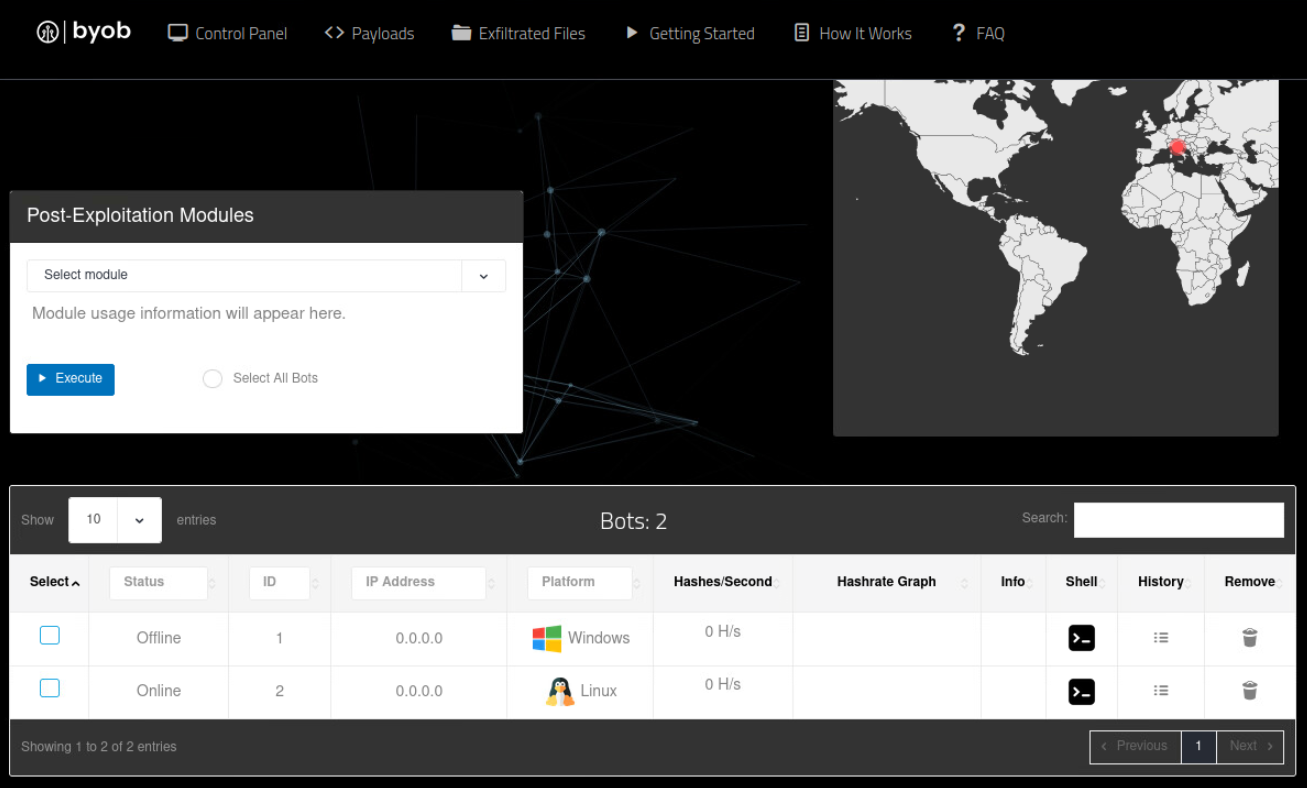
\includegraphics[width=\textwidth, height=6cm]{res/fig/byob-home.png}
        \caption{}
        \label{fig:byobhome}
    \end{subfigure}
    \hfill
    \begin{subfigure}[hbtp]{0.45\textwidth}
        \centering
        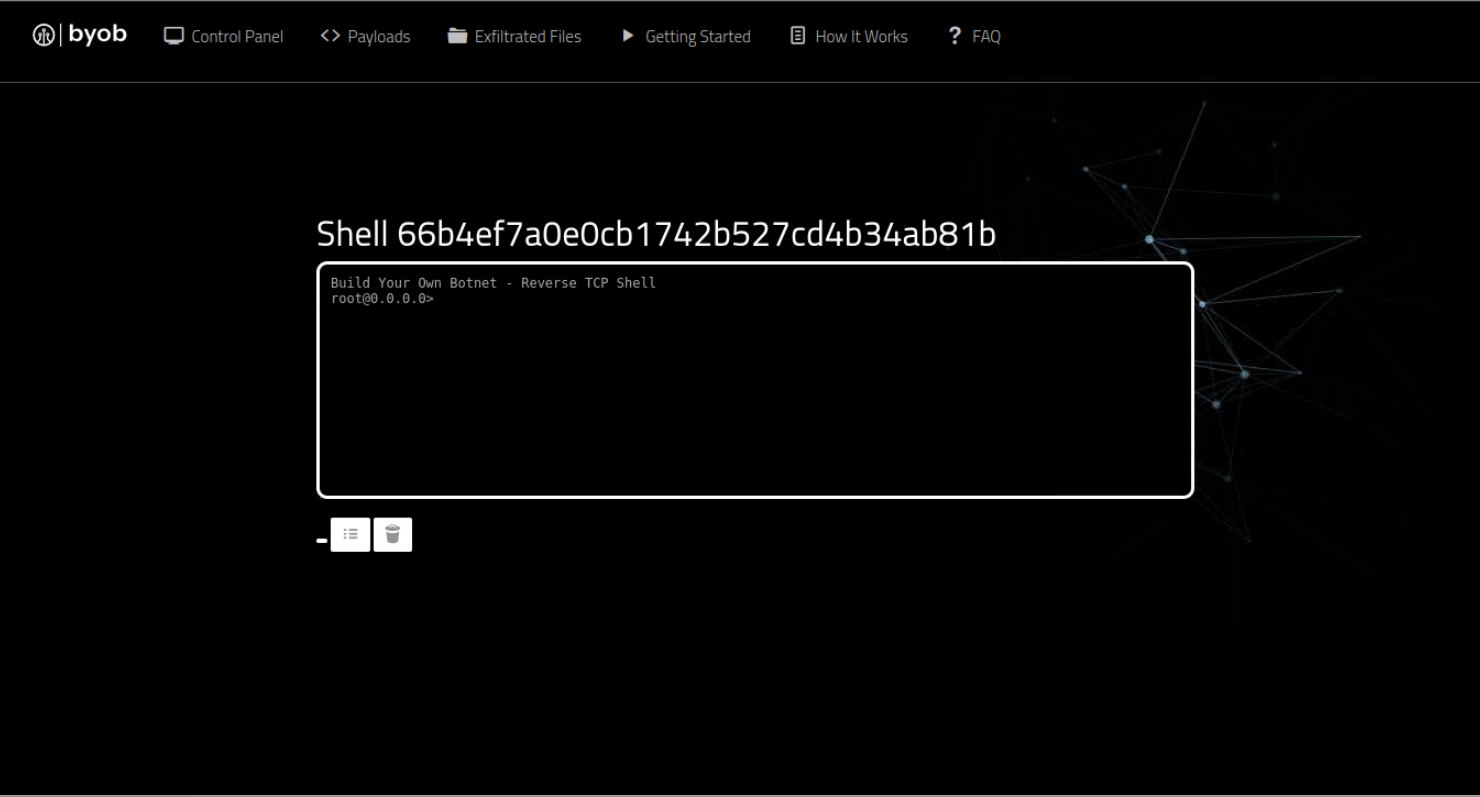
\includegraphics[width=\textwidth , height=6cm]{res/fig/byob-shell.png}
        \caption{}
        \label{fig:byobshell}
    \end{subfigure}
    \caption{(a) Home page; (b) Pagina shell.}
    \label{ciao1}
\end{figure}

L'interfaccia web del C\&C è  dotato di sistema di autenticazione, per impedire che terzi possano prenderne il controllo facilmente. Quindi prima di poter interagire con le funzionalità che offre l'interfaccia web è necessario eseguire il login nell'apposita pagina web.
Nella \Cref{fig:byobhome}  si può vedere la schermata di controllo principale dell'interfaccia web di Byob. In basso è presente una schermata con i bot attualmente collegati. Sul lato  sinistro vi è  un pannello con i moduli di post-exploitation utilizzabili sui bot del pannello sottostante, mentre a destra si può controllare la posizione geografica del bot. 

Cliccando sull'icona del terminale in corrispondenza di un bot nel pannello inferiore, reindirizza il browser verso una schermata in cui viene emulato un terminale. Questo è collegato al bot attraverso reverse-shell e può essere usato per operare direttamente sul bot.
\begin{figure}[hbtp]
    \centering
    \begin{subfigure}{0.45\textwidth}
        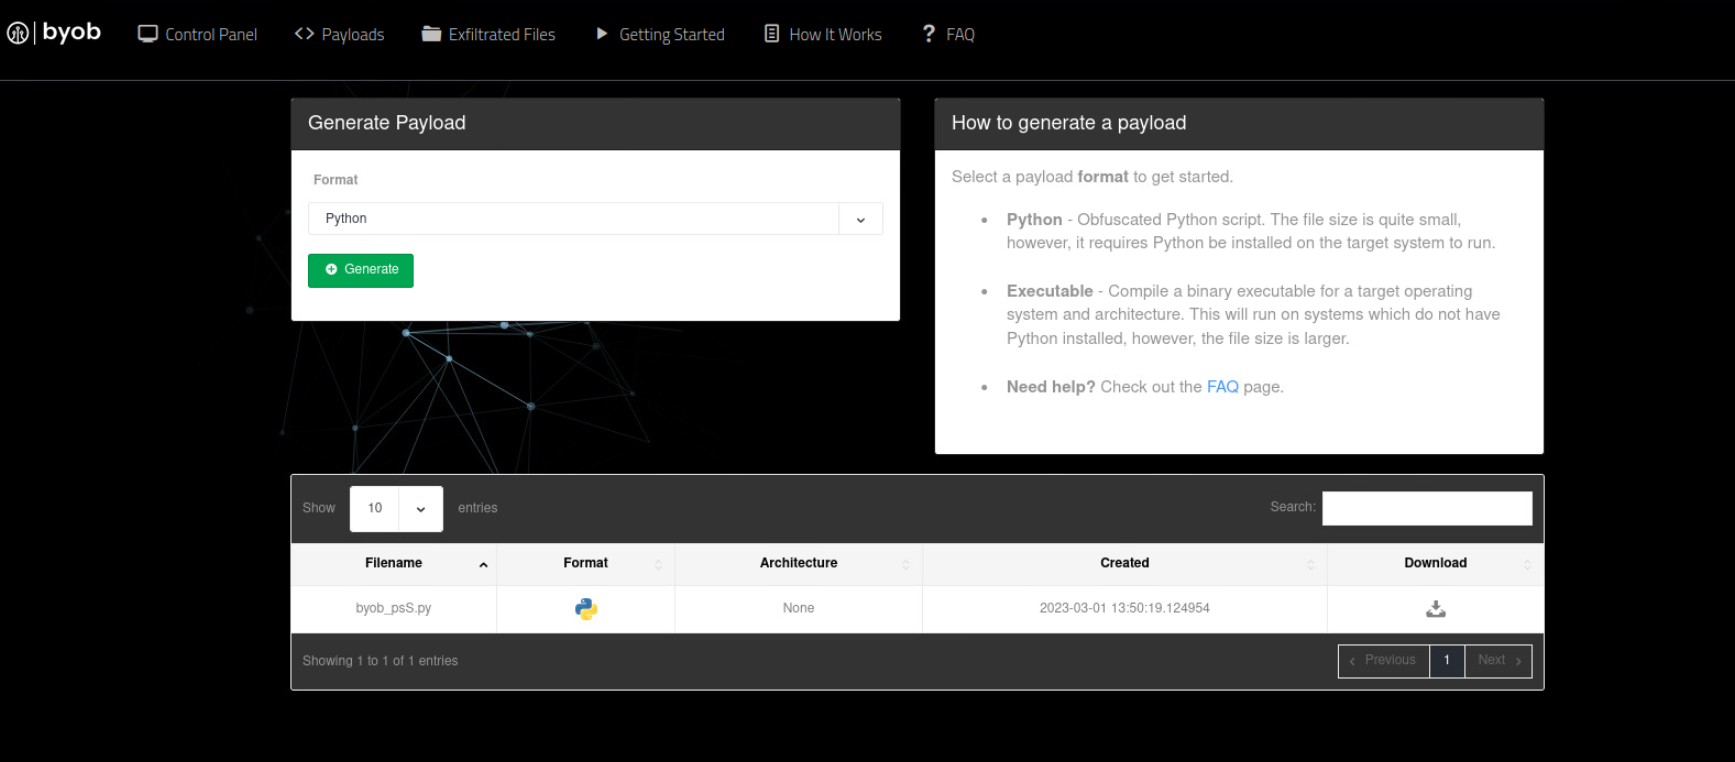
\includegraphics[width=\textwidth , height=6cm]{res/fig/byob-payloads.png}
        \caption{}
        \label{fig:byobpayloads}
    \end{subfigure}
    \hfill
    \begin{subfigure}{0.45\textwidth}
        \centering
        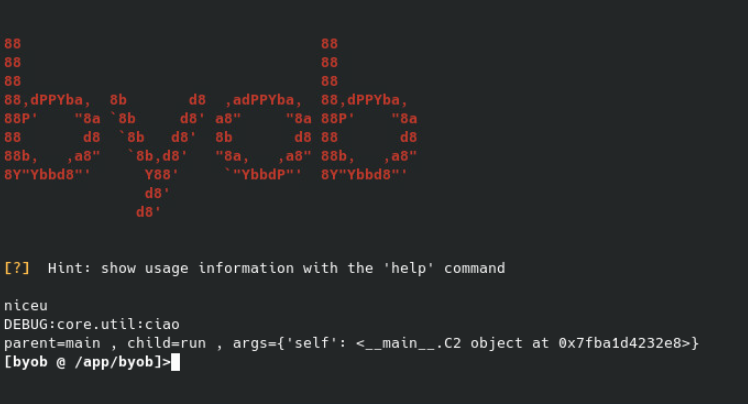
\includegraphics[width=\textwidth , height=6cm]{res/fig/byob-console.png}
        \caption{}
        \label{fig:byobconsole}
    \end{subfigure}
    \caption{(a) Schermata di generazione dei payload; (b) Byob console.}
    \label{ciao2}
\end{figure}

In \Cref{fig:byobpayloads} si può osservare la schermata di creazione dei payload. I payload possono essere eseguibili compilati o script Python. Una volta creati possono essere scaricati da questa pagina web.

Byob può essere anche eseguito nella sua variante minimale da console (\Cref{fig:byobconsole}).


Attraverso il pannello di controllo o le console è possibile controllare i bot ed eseguire le classiche funzionalità RAT o eseguire moduli Python arbitrari, rendendo di fatto possibile eseguire qualsiasi operazione\footnote{per alcune operazioni può essere necessaria l'autenticazione come amministratore.} sulle macchine vittime.


\section{Dettagli implementativi}
Nella seguente sezione verranno descritti più nel dettaglio i principali componenti su cui è basata la botnet.

\subsection{Server}
Lo script \textit{Server.py} è il responsabile dell'esecuzione del server e di tutte le sue funzionalità. In \Cref{fig:byobumlserver} si può vedere un diagramma di sequenza che ne descrive il comportamento.

Al momento dell'esecuzione crea tre sottoprocessi che eseguiranno in background:
\begin{description}
    \item[Packages handler] Mantiene un server HTTP su porta dedicata incaricato di fornire i Python Package richiesti da bot;
    \item[Module handler] Mantiene un server HTTP su porta dedicata incaricato di fornire Moduli Python richiesti da bot;
    \item[Request handler] Gestisce le richieste POST di upload  inviate da bot, salvando i file in apposite directory.
\end{description}
Successivamente, esegue il C\&C server su un'altra porta dedicata.
Il C\&C server crea un thread che si occupa di gestire le nuove connessioni inizializzate dai bot. Per ogni nuovo bot connesso crea una sessione, cui informazioni vengono salvate in database e aggiornate a ogni connessione. 

Una volta creato il thread, si occupa di gestire i comandi inseriti su console di controllo dei bot e le richieste  dell'interfaccia web.
Come già osservato nell'introduzione di questo capitolo, Byob può eseguire anche senza interfaccia web e in tal caso la console non è inizialmente collegata a un bot. La console emulata dell'interfaccia web, invece, è già associata al bot specifico. 

Quando Byob esegue in console, ha a disposizione dei comandi, di cui la versione con interfaccia web non ha bisogno, dato che sono integrati all'interno delle pagine web (eg. controllare le sessioni attive).

Durante il ciclo di vita del C\&C, la console  rimane in attesa di input. Quando viene inserito un comando,  ne effettua il parsing per controllare che sia un comando disponibile e nel caso lo esegue con eventuali parametri annessi.
 Una volta collegata alla sessione del bot, questa rimane in attesa di comandi da inoltrare. 
 La versione web usa uno script Javascript per inviare una richiesta POST contenenti i comandi digitati al backend che si occupa di inoltrarlo al bot.
 La versione console invece crea un thread che è incaricato di inviare i comandi direttamente al bot, e li inoltra solo in risposta a richieste di polling da parte del bot.
 Si può quindi affermare che la versione web sia push-based mentre l'altra pull-based.
 
 Da questo punto in avanti le funzionalità di console e  console web emulata sono identiche, la versione web infatti sfrutta le funzionalità riadattate di Byob versione console.

Il server invia comandi e riceve risultati sotto forma di dizionari contenenti altre informazioni come l'id del bot.


\begin{figure}
    \centering
    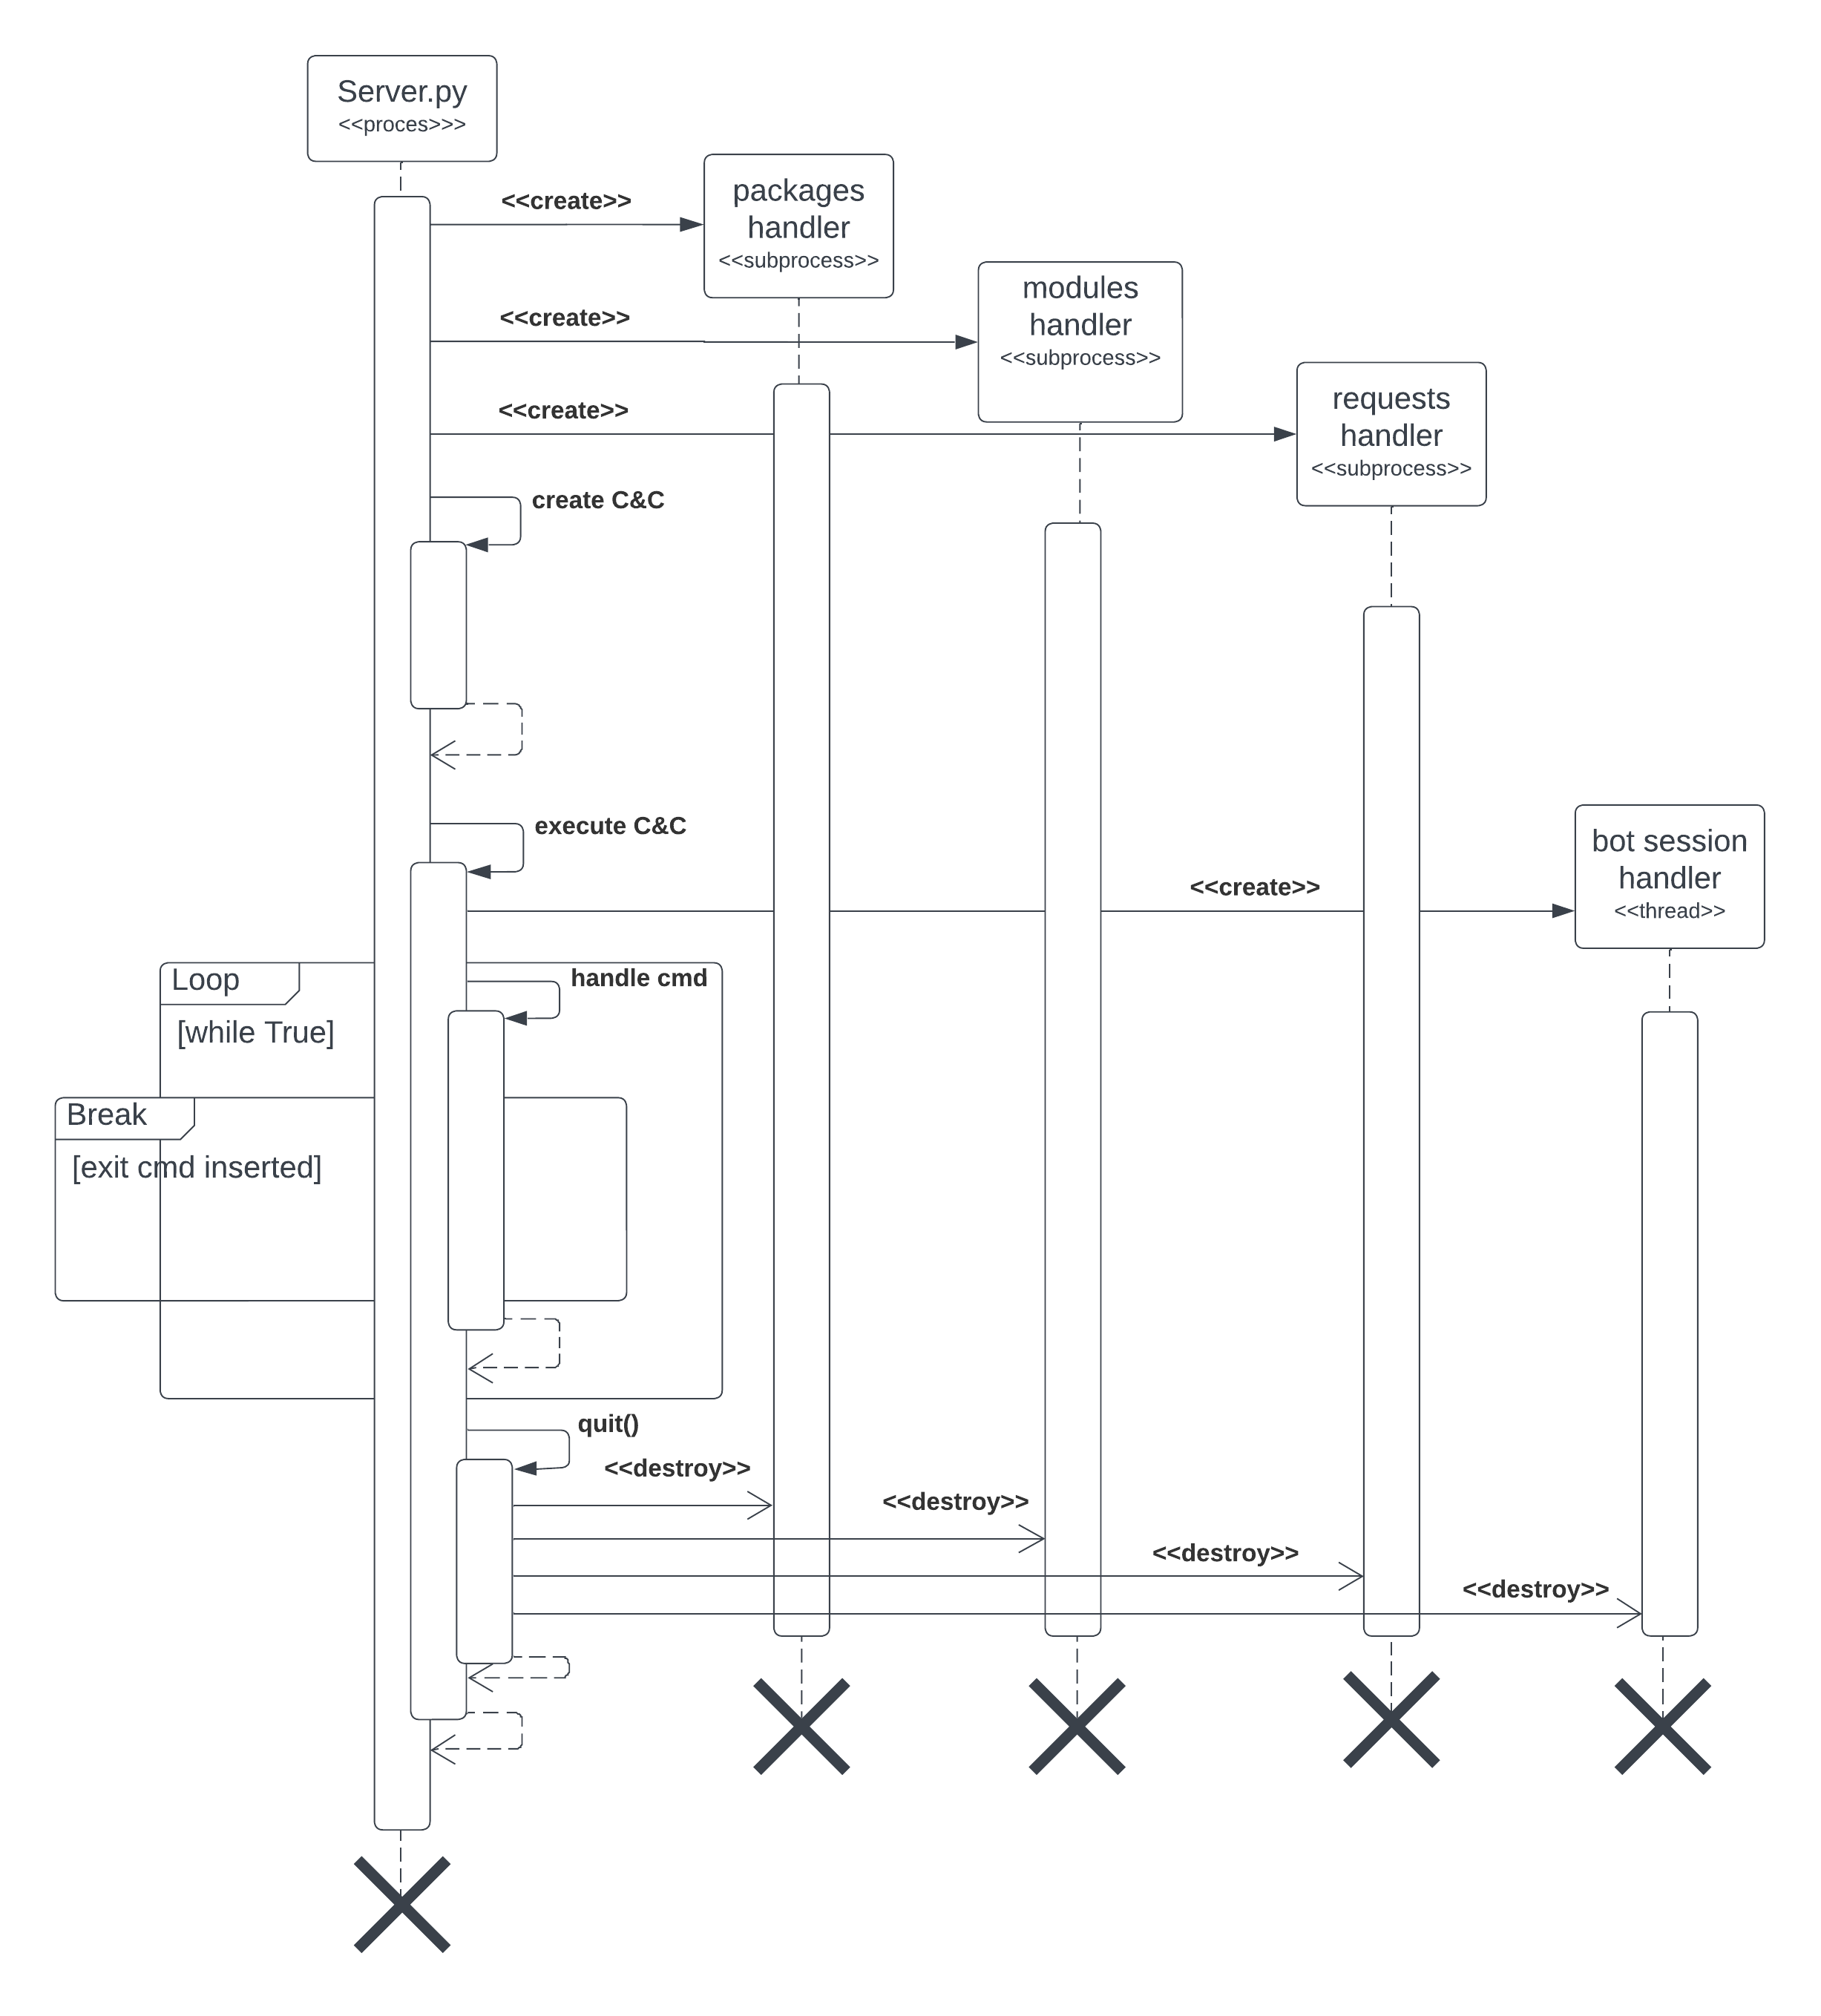
\includegraphics[width=\textwidth]{res/fig/byob-uml-server.png}
    \caption{Diagramma di sequenza di Byob.}
    \label{fig:byobumlserver}
\end{figure}


\subsection{Payload}

L'infezione attraverso payload è strutturata su più parti consequenziali.

Il file che la vittima esegue è il \textit{Dropper}.
Il Dropper scarica dal server lo Stager e lo esegue. Le righe di codice Python responsabili del download sono inizialmente serializzate, compresse e codificate in base64, per rendere più difficile l'identificazione di codice malevolo da parte strumenti di rilevazione.

Lo Stager, a sua volta, scarica il Payload dal server.  Di default il server invia il payload in chiaro, ma è possibile criptare il contenuto del Payload, in questo caso lo Stager si preoccupa di decriptarlo prima di eseguirlo.

Il Payload è il cuore del malware.

Una volta eseguito instaura una connessione col server e inizializza due thread, incaricati di ricercare e importare  moduli e package da remoto, per poi entrare in un loop in attesa di task da eseguire.

Alla ricezione di un task,  esegue il parsing e ne esegue comando, cui  risultato viene incapsulato e inoltrato al server.
Nel caso il server operi  senza interfaccia web, viene eseguito un thread incaricato di eseguire polling verso il server, a cui il server occasionalmente risponderà con un task.

In caso la ricezione del comando fosse un modulo, questo viene importato da remoto e inseguito eseguito.

L'importazione di un modulo (o package) avviene aggiungendo un oggetto di classe Loader, contenenti i metodi \textit{find\_module} e \textit{load\_module}, alla lista di oggetti \textit{sys.meta\_path} e in seguito eseguendo l'import manuale del modulo. 
Normalmente, quando l'interprete Python cerca di importare un modulo, naviga la lista \textit{sys.meta\_path} ed esegue il metodo \textit{find\_module} di ciascun oggetto. Questo metodo restituisce un loader del modulo selezionato nel caso lo trovi. Un loader è un oggetto che implementa il metodo \textit{load\_module}.
Una volta che il loader è stato trovato, ne viene eseguito il metodo \textit{load\_module} che importa il modulo all'interno del contesto.

Byob sfrutta questo meccanismo. Quando esegue l'import manuale di un modulo remoto, l'interprete si imbatte nel loader inserito da Byob all'interno della lista \textit{sys.meta\_path} ed esegue il suo metodo di ricerca. Questo cerca il modulo all'interno della lista di moduli disponibili precedentemente estratta dal server, e nel caso lo trovi ritorna un'istanza di se stesso. Dato che la classe loader di Byob è fornita anche del metodo \textit{load\_module}, può eseguirlo per importare il modulo da remoto.


Quando il bot è incaricato di eseguire l'upload di un file verso il server, invia una richiesta POST al sottoprocesso del server, incaricato di gestire le richieste POST, sulla porta dedicata.

\section{Testing e debug}
Per eseguire il testing, il server è stato containerizzato con Docker.
Il build dell'immagine è stato eseguito attraverso il seguente Dockerfile:
\lstset{  basicstyle=\footnotesize,
frame=single}
\begin{lstlisting}[caption={Byob server Dockerfile.},label={listing-byobdocker},frame=single]
FROM ubuntu:bionic

WORKDIR /app
COPY . .
RUN apt-get update && \
    apt-get upgrade -y && \
    apt-get install -y build-essential cmake && \
    apt-get install -y python3.6 python3-pip && \

WORKDIR /app/web-gui
RUN python3.6 -m pip install pip --upgrade && \
    python3.6 -m pip install -r requirements.txt && \
    rm -rf .gitignore .travis.yml README.md requirements.txt \
        startup.sh docker-pyinstaller*

EXPOSE 5000 1337 1338 1339
ENTRYPOINT python3.6 run.py --debug
\end{lstlisting}
Il Dockerfile specifica che al momento del build deve essere copiato il sorgente del server all'interno del container, che devono essere installate tutte le dipendenze necessarie e che devono essere esposte le porte 5000, 1337, 1338, 1339 del Container.
Per eseguire  il container contenente il server è stato utilizzato  il seguente \textit{bash} script:
\begin{lstlisting}{caption={Bash script per eseguire Byob in Docker Container.},label={listing-byobscript1}}
containers=`docker ps -a | grep -A 1 byob | cut -b -12`;
for x in $containers; do 
    docker stop $x && docker rm $x ;
done;
docker run --name byob-web -it  -p 5000:5000 -p 1337:1337 \
    -p 1338:1338 -p 1339:1339 -v ./byob:/app   byobserver ;
\end{lstlisting}
Lo script interrompe l'esecuzione di tutti i container Byob esistenti e li rimuove prima di eseguire un nuovo container. La porta 5000 dell'host viene mappata alla porta del C\&C  mentre le restanti sono mappate ai servizi di distribuzione dei moduli/package e    gestione delle richieste POST. La directory contenente il sorgente è stata mappata a una directory dell'host in modo che fosse facile modificarne il codice all'occorrenza e per fare in modo che alla rimozione del container la directory fosse persistente sulla macchina host. Gli argomenti \textit{-it} sono utilizzati per rendere possibile l'interazione con la shell di debug del container.

Purtroppo il software ha presentato diversi problemi e bug da risolvere nella sua versione \textit{out of the box}. 

La funzionalità di import dei   package da remoto risulta rotta. In particolare la ricerca confonde i moduli con i package,  non riuscendo quindi mai a trovare ciò che si desidera poi importare. Il problema è stato aggirato ma non risolto, evitando di perdere troppo tempo su questioni secondarie, importando manualmente da locale i package necessari.

I moduli di post-exploitation sono compatibili solo con alcuni degli OS e la maggior parte risultava non funzionante. 
La botnet è stata testata sia con bot Windows che con bot Linux.
Tra i moduli  testati e non funzionanti vi sono i moduli per eseguire screenshot, keylogging, cattura del traffico di rete e uso della  Webcam.

Analizzando il modulo Keylogger si è potuto notare che il modulo risulta scritto in modo errato, forse perché utilizza una versione deprecata di API della libreria che sfruttava per eseguire il suo compito. 

Tra i moduli che invece risultano funzionanti vi erano quello utilizzato per eseguire scansioni delle porte di rete e quello per la gestione dei processi.

Le funzionalità di RAT funzionano correttamente.
In particolare è stata testata l'esecuzione di codice Python arbitrario attraverso riga di comando o  attraverso l'import di moduli creati appositamente.

La  creazione del Payload criptato non funziona correttamente.


Le funzionalità di geolocalizzazione, l'import di script di Google Analytics e font scaricati da Internet sono stati rimossi in quanto si appoggiano a servizi web esterni non raggiungibili dall'interno del perimetro di testing, provocando  il crash dell'applicativo e ritardi nell'esecuzione.



A seguito di una fase di risoluzione dei problemi che ha richiesto un considerevole impiego di tempo, si è ritenuto opportuno procedere alla verifica con IDS delle sole funzionalità che al momento risultavano operative, per poi procedere con lo studio di un'ulteriore botnet.

\section{Rilevazioni con IDS}


In \Cref{fig:byob-result-1} si possono vedere gli eventi generati da Security Onion attraverso il modulo Suricata al momento dell'esecuzione del Payload. Gli eventi sono autoesplicativi e fanno riferimento in particolare a:
\begin{itemize}
    \item Download di eseguibile;
    \item Richiesta web verso indirizzo IP;
    \item Rilevazione di Python all'interno dello user-agent;
    \item Rilevazione di codice di classe Loader di Byob;
    \item Rilevazione di codice di Stager di Byob.
\end{itemize}

\begin{figure}[hbtp]
    \centering
    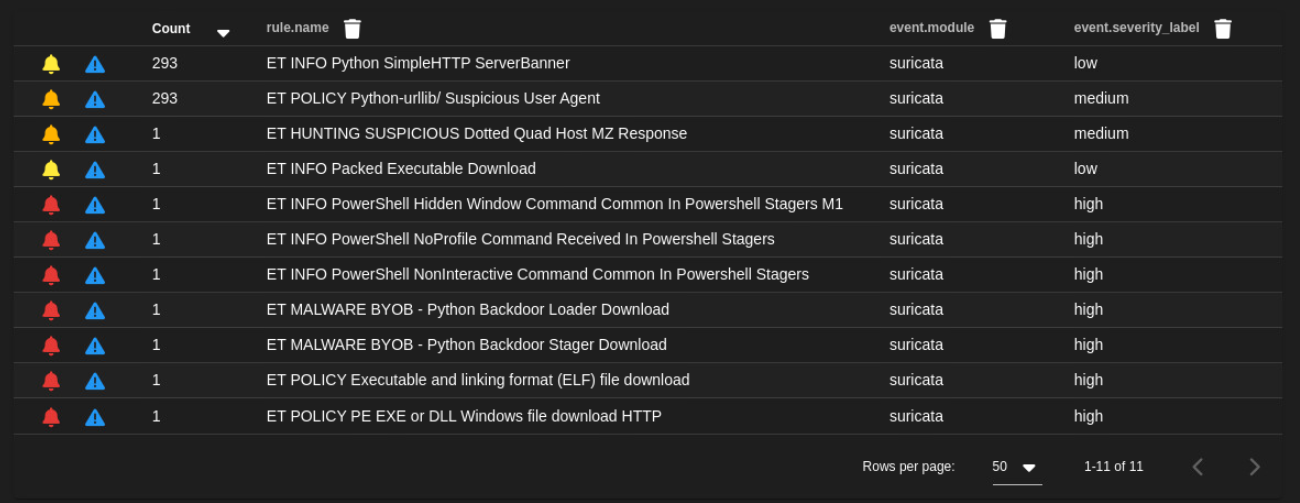
\includegraphics[width=\textwidth]{res/fig/byob-result-1.png}
    \caption{Rilevazione Security Onion dell'esecuzione del Payload.}
    \label{fig:byob-result-1}
\end{figure}

Gli eventi più significativi fanno riferimento alla rilevazione di eseguibili e codici maligno noto. Se il download del payload fosse stato criptato nessuna di queste rilevazioni   avrebbe avuto luogo tranne il riferimento all'indirizzo IP.

In \Cref{fig:byob-results-2-3} si possono osservare le rilevazioni di Security Onion e Ossim in merito all'esecuzione del modulo di scansione di rete.

Le funzionalità di RAT attraverso reverse-shell e l'utilizzo di moduli Python generici costruiti ad-hoc non sono stati rilevati.
Questo perché  Suricata non ha fingerprint che facciano riferimento ai moduli da noi creati, mentre i comandi inoltrati attraverso reverse-shell sono criptati con AES-256 e non vi è modo di identificare quel traffico di rete come maligno sfruttando solo SIDS.
%inserire test con import di miner che strelka dovrebbe rilevare specificando che import non è criptato e quindi può leggere.

Seppure il modulo di mining non sia stato testato a pieno, in quanto richiedeva interazioni con la rete Internet, al momento dell'esecuzione il download dell'eseguibile di un noto malware dal C\&C. Essendo un malware noto, di cui esistono fingerprint in database pubblici, Strelka è stato in grado di identificarlo come si può osservare da una sezione del log riportato in \Cref{fig:byob-results-4}.


\begin{figure}[hbtp]
    \centering
    \begin{subfigure}{\textwidth}
        \centering
        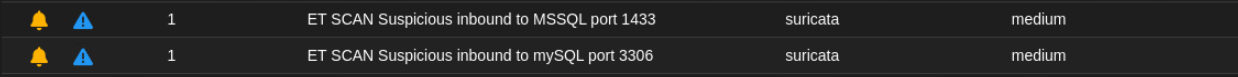
\includegraphics[width=\textwidth]{res/fig/byob-result-2.png}
        \caption{Security Onion.}
        \label{fig:byob-result-2}
    \end{subfigure}
    \hfill
    \begin{subfigure}{\textwidth}
        \centering
        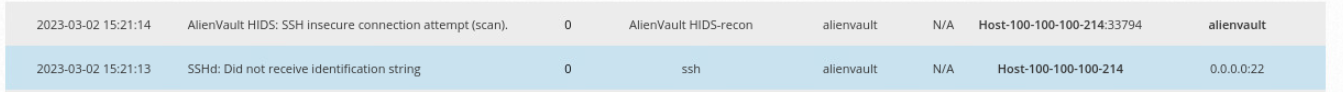
\includegraphics[width=\textwidth]{res/fig/byob-result-3.png}
        \caption{Ossim.}
        \label{fig:byob-result-3}
    \end{subfigure}
    \caption{Rilevazioni della scansione di rete eseguita da bot attraverso modulo apposito.}
    \label{fig:byob-results-2-3}
\end{figure}
\begin{figure}[hbtp]
    \centering
    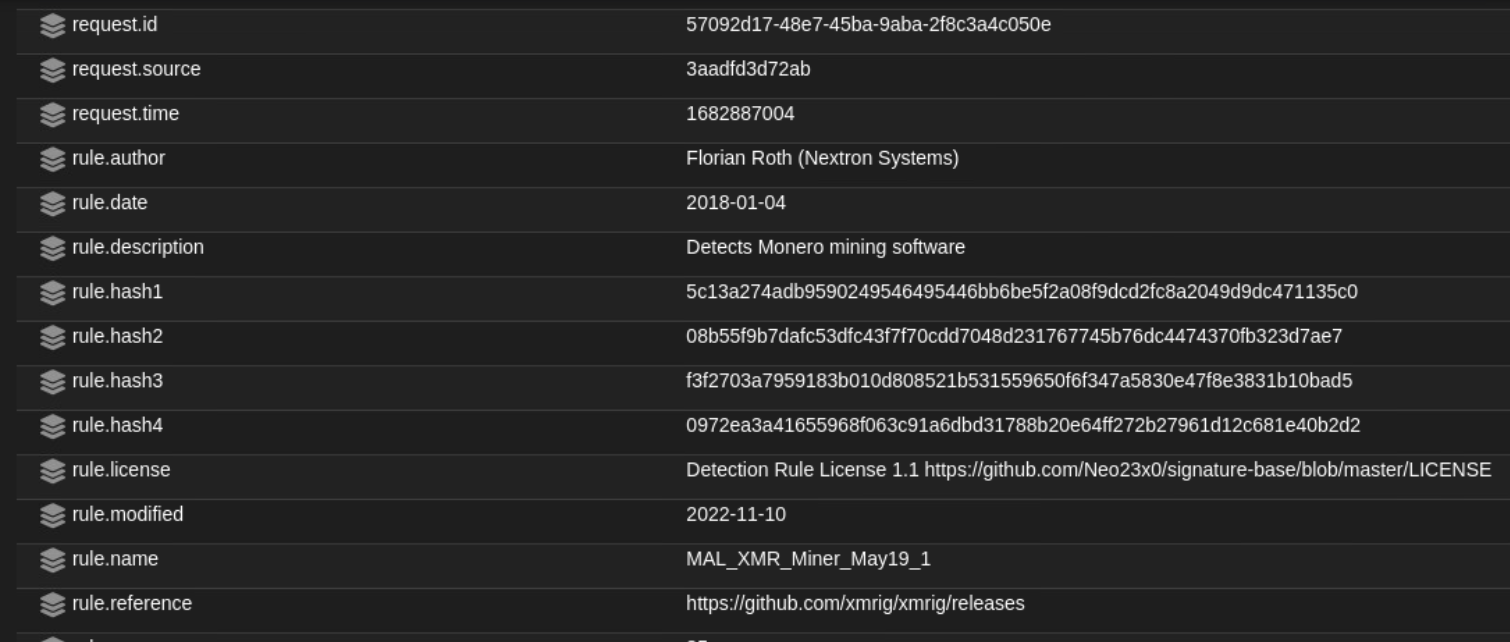
\includegraphics[width=\textwidth]{res/fig/byob-strelka.png}
    \caption{Rilevazione di import di malware noto.}
    \label{fig:byob-results-4}
\end{figure}


\chapter{Agent}
Un agente o agent è un software  definito a largo modo  come un programma che può esercitare l'autorità di un individuo o di un'organizzazione, lavorare autonomamente per raggiungere un obiettivo e interagire con altri agenti e con l'ambiente circostante \cite{jansen2002intrusion}. 
Esso si compone di codice e informazioni sullo stato del sistema per seguire computazioni. Inoltre, richiede una piattaforma sui cui eseguire.
%here1

Gli agent possono essere statici o mobili. Quelli statici rimangono fissi in una singola piattaforma mentre quelli mobili sono in grado di fermare la computazione, spostarsi su un'altra piattaforma e riprendere con l'esecuzione del proprio codice.

La piattaforma d'origine di un agent è chiamata \textit{home platform} e normalmente è l'ambiente considerato più sicuro per l'agent.
Una piattaforma può avere molteplici luoghi in cui più agent possono interagire.

La tecnologia degli agenti mobili ha tratto beneficio dal lavoro svolto sugli agenti intelligenti e sullo sviluppo di sistemi software capaci di supportare codice su hardware eterogeneo (eg. Java e Java Virtual Machine sono un esempio di sistema software capace di portare codice eseguibile su qualsiasi sistema operativo). Con agente intelligente si intende  agenti statici autonomi capaci di applicare la conoscenza del dominio dell'applicazione. Gli agenti intelligenti incorporano la capacità di decomporre e risolvere problemi in modo collaborativo. Gli agenti osservano il loro ambiente, ragionano sulle proprie azioni e su quelle degli altri agenti, interagiscono con altri agenti ed eseguono le proprie azioni in modo concorrente con altri agenti.
 Attraverso le interazioni possono scambiarsi informazione tramite un linguaggio di comunicazione degli agenti e possono collaborare per creare una conoscenza comune su un argomento.

Anche se gli agenti mobili mantengono le caratteristiche di autonomia e collaborazione degli agenti intelligenti, l'accento è sulle caratteristiche di mobilità, spesso basandosi su algoritmi semplici e diretti per il ragionamento e la collaborazione attraverso una meno elaborata interpretazione dei messaggi.


La capacità di spostare una computazione tra diversi nodi offre vantaggi rispetto agli attuali sistemi di rilevamento delle intrusioni che si basano su computazioni staticamente posizionate. Per poter applicare la tecnologia degli agenti mobili alla rilevazione delle intrusioni, i nodi partecipanti (cioè gli host e i dispositivi di rete) devono avere installata una piattaforma per agenti. Poiché molti sistemi di agenti funzionano su una vasta gamma di hardware e software, questo requisito non è difficile da soddisfare. Con la tecnologia degli agenti mobili, i nodi di raccolta, di aggregazione interna e di comando e controllo non devono essere continuamente residenti sulla stessa macchina fisica. Ad esempio, un agente mobile può funzionare come nodo di aggregazione e spostarsi in qualsiasi posizione fisica nella rete che sia migliore per i suoi scopi. Il paradigma degli agenti mobili offre inoltre la possibilità di specializzazione: gli agenti possono essere diversi per funzioni diverse, ognuno alla ricerca di attacchi distinti e di conseguenza elaborando i dati in modo specifico.


La tecnologia degli agenti mobili può potenzialmente superare alcune limitazioni intrinseche degli IDS  che utilizzano solo componenti statici. Ciò non significa che le caratteristiche degli agenti mobili in sé siano sufficienti per ottenere miglioramenti. Quando si applicano agenti mobili a questo dominio di applicazione, sono comunque necessarie scelte di progettazione accurate per sfruttare le loro caratteristiche. In particolare, il tipo di coordinamento del livello di conoscenza richiesto per rilevare e rispondere alle intrusioni pone molte esigenze sugli agenti, tra cui localizzare altri agenti con le capacità necessarie, comunicare efficacemente con loro utilizzando un vocabolario comune e coordinare le azioni da intraprendere per affrontare congiuntamente una situazione data. In passato sono stati identificati diversi vantaggi nell'utilizzo degli agenti mobili rispetto ai loro omologhi statici \cite{lange1998mobile,smith1988survey,vuong2011advanced}:

\begin{description}
    \item [Diminuire la latenza di rete] Grazie alla loro capacità di essere inviati per eseguire operazioni direttamente al punto di interesse remoto, gli agenti mobili sono in grado di rispondere in tempo reale ai cambiamenti dell'ambiente. Oltre a rilevare e diagnosticare potenziali intrusioni di rete, gli agenti mobili possono fornire meccanismi di risposta adeguati, tra cui la raccolta di informazioni sull'attacco inviate al bersaglio o emesse da esso, la chiusura o l'isolamento di un sistema sotto attacco per proteggerlo da ulteriori danni, il tracciamento del percorso dell'attacco e la chiusura o l'isolamento del sistema dell'attaccante se l'attacco viene lanciato da un host interno;
    \item[Ridurre il carico di rete] Piuttosto che trasferire i dati attraverso la rete per eseguire computazioni su questi, gli agenti mobili possono essere inviati direttamente alla macchina in cui risiedono i dati, portando il la computazione vicino ai dati invece di dover spostare i dati  verso la computazione. Ciò consente di ridurre il carico sulla rete;%Inoltre, in caso la confidenzialità sia una necessità, spostare un agente crittografato e i suoi dati elaborati può risultare più efficiente rispetto al trasferimento di tutti i dati grezzi in forma crittografata.
    \item [Esecuzione autonoma e distribuita] Per grandi sistemi distribuiti, è essenziale la capacità del sistema di continuare a funzionare quando parti di esso vengono distrutte o vengono isolate. Gli agenti mobili possono esistere e funzionare in modo indipendente dalla piattaforma di creazione, rendendoli utili come componenti di IDS, poiché gli agenti che sopravvivono a un attacco potrebbero essere in grado di ricostituire le componenti danneggiate (ad esempio, clonandole) e ripristinare la funzionalità;
    \item [Adattamento dinamico] I sistemi di agenti mobili sono in grado di rilevare il proprio ambiente e adattarsi ai cambiamenti, rendendoli particolarmente utili nella rilevazione delle intrusioni. Gli agenti possono muoversi in modo autonomo per migliorare la loro posizione o evitare situazioni pericolose, clonarsi per garantire la ridondanza e l'esecuzione parallela, o unirsi ad altri agenti per ottenere assistenza. Inoltre, possono adattarsi in modo flessibile a situazioni sfavorevoli o favorevoli. Grazie alla loro esecuzione autonoma e asincrona, queste caratteristiche consentono di costruire sistemi robusti e in grado di tollerare i guasti;
    \item [Indipendenza dalla piattaforma]  I sistemi di agenti forniscono un ambiente di calcolo astratto per gli agenti, indipendente dall'hardware e dal software del computer su cui viene eseguito. Queste caratteristiche rendono questo ambiente un'opzione adatta per le applicazioni di gestione di rete in generale e di rilevazione delle intrusioni in particolare, permettendo agli agenti di muoversi relativamente liberamente all'interno di un dominio. Questo è particolarmente vantaggioso per i meccanismi di risposta, poiché quando viene rilevata un'intrusione, i rimedi possono essere applicati o avviati da quasi qualsiasi punto della rete. Inoltre, i meccanismi di rilevamento beneficiano della mobilità diffusa degli agenti, che ha il potenziale di acquisire e unire facilmente dati da diverse fonti di rete;
    \item [Software upgrade] Per aggiornare il software su più host, di solito l'amministratore deve fermare il server, disinstallare la vecchia versione del software e reinstallare la nuova versione. Ciò comporta la necessità di fermare l'intero sistema software. Tuttavia, se ogni componente del software è gestito da un agente, è possibile semplicemente disabilitare l'agente vecchio e distribuire un nuovo agente con le funzionalità richieste, senza interrompere l'intero sistema. Questo approccio consente di fermare solo il componente basato su agente che necessita di aggiornamento, evitando di fermare l'intero sistema.
\end{description}


Anche se il nostro interesse è associare gli  agenti mobili alla rilevazione delle intrusioni, è improbabile che la piena mobilità di tutti i componenti di un IDS sia  efficace in pratica, a causa dell'eccessivo overhead associato. Pertanto, alcuni componenti dell'IDS vengono designati come agenti statici o rimangono statici una volta implementati. Ciò consente l'applicazione del paradigma dell'agente mobile, ma si basa sulla mobilità solo dove appropriato.

\smallskip

Gli agenti mobili non migliorano direttamente le tecniche di rilevamento, ma possono modellare l'applicazione di tali tecniche migliorandone l'efficienza e l'efficacia. Un'area di potenziale utilizzo è la riduzione dell'enorme quantità di dati di log distribuiti tra i nodi interni di un sistema IDS convenzionale. I mobile agent possono visitare i repository dei dati e analizzare i risultati, trasferendo il calcolo ai dati stessi. Questo approccio riduce il carico di rete e consente agli agenti specializzati di concentrarsi su classi specifiche di intrusioni.

Un altro utilizzo dei mobile agent è la minimizzazione della capacità di un attaccante di ingannare un IDS. Gli agenti possono replicarsi e risiedere su più piattaforme, eliminando tali tentativi. Passare da IDS basati su rete ad agenti di rilevamento basati su host che funzionano contemporaneamente riduce anche la possibilità di pacchetti persi e massimizza la possibilità di innescare una risposta rapida a una intrusione rilevata. Inoltre, avere componenti residenti sull'host fornisce l'unico modo per l'IDS di visualizzare i pacchetti in testo normale, nelle situazioni in cui l'host utilizza la crittografia a livello di rete.

I mobile agent possono agevolare l'implementazione di architetture IDS robuste e resistenti agli attacchi \cite{mell2000denial}. Gli agenti si spostano quando rilevano pericolo o attività sospette, si clonano per garantire la ridondanza o la sostituzione, operano autonomamente e in modo asincrono rispetto al luogo di creazione, collaborano e condividono conoscenze, e si auto-organizzano per ovviare ad anomalie. Inoltre, gli agenti si prestano alla diversità genetica, che aiuta a evitare attacchi mirati a eludere i meccanismi di rilevamento noti e stabili dell'IDS.

Il maggior potenziale dei mobile agent risiede nella risposta a un'incursione piuttosto che nel suo rilevamento. Poiché le risposte possono essere avviate da quasi ovunque nella rete, i mobile agent possono gestire gli attacchi in modo più ottimale rispetto a un IDS convenzionale.

Alcuni dei vantaggi nell'implementare un mobile agent per rispondere a intrusioni possono essere:
\begin{description}
    \item [Tracciatura di un attaccante] Gli attaccanti spesso si insinuano all'interno di una catena di molti host prima di attaccare l'obiettivo e generalmente falsificano l'indirizzo di origine. Per trovare l'attaccante l'IDS deve ispezionare la catena di host per trovare il responsabile dell'inoltro dei pacchetti considerati come maligni. Per eseguire una tale traccia l'IDS deve essere in grado di analizzare il traffico di rete di ogni segmento di rete e ogni host. In genere tale compito sarebbe troppo dispendioso ma è realizzabile  con una base di agent abbastanza ampia;
    \item [Risposta in host target] Quando un attacco viene rilevato è importante poter rispondere alla minaccia all'interno dell'host colpito. Ciò è effettuabile attraverso gli agent;
    \item [Risposta in sorgente di attacco] Una possibile riformulazione più fluida potrebbe essere: "Per limitare le azioni dell'attaccante, l'IDS può agire direttamente sul suo host, ma ciò richiede l'uso di agenti mobili, altrimenti l'accesso sarebbe limitato. Nonostante questa opzione abbia delle restrizioni, come la necessità che l'attacco provenga dall'interno del dominio di gestione, può comunque essere un'arma molto efficace per l'IDS;
    \item [Raccolta di evidenze] Al momento, è difficile raccogliere automaticamente prove di attacchi provenienti da molteplici fonti. Ciò è dovuto alla necessità di avere il software adatto eseguito nel luogo e nel momento giusto. Tuttavia, gli agenti mobili possono essere utilizzati per eseguire qualsiasi cosa in qualsiasi momento e ovunque, rendendo possibile la raccolta di prove da diverse piattaforme hardware, sistemi operativi e persino applicazioni come i server web;
    \item[Isolamento di target e attaccante] Poiché le azioni per rispondere automaticamente al bersaglio e alla fonte possono fallire, è necessaria  una risposta a livello di rete per limitare le azioni di un attaccante. Ci sono tre strategie generali: bloccare le comunicazioni del bersaglio, bloccare le comunicazioni dell'attaccante e bloccare le comunicazioni tra il bersaglio e l'attaccante. Grazie alla loro capacità di viaggiare in tutti gli elementi della rete per eseguire azioni correttive, gli agenti mobili sono in grado di attuare tali strategie.
\end{description}

\smallskip
Il principale ostacolo nell'utilizzo di agenti mobili per la rilevazione delle intrusioni è la sicurezza. L'uso di agenti mobili può introdurre vulnerabilità che possono essere sfruttate da un attaccante per propagare un attacco o sovvertire la rilevazione dell'IDS. Le minacce alla sicurezza per il paradigma di elaborazione degli agenti mobili possono essere classificate in quattro categorie:
\begin{description}
    \item [Da agente ad agente] Si verificano quando gli agenti sfruttano le debolezze di sicurezza o lanciano attacchi contro altri agenti che risiedono in stessa piattaforma;
    \item [Da agente a piattaforma]  Si verificano quando gli agenti sfruttano le debolezze di sicurezza o lanciano attacchi contro una piattaforma di agenti in cui risiedono;
    \item [Da piattaforma ad agente]  Si verificano quando le piattaforme di agenti compromettono la sicurezza degli agenti che risiedono lì;
    \item [Da altri a piattaforma] si verificano quando entità esterne, inclusi agenti e piattaforme di agenti situati altrove sulla rete, minacciano la sicurezza di una piattaforma di agenti, inclusi il suo sistema operativo sottostante e il servizio di comunicazione di rete.
\end{description}

\smallskip

In linea di principio, queste minacce non sono diverse da quelle che affrontano altre applicazioni distribuite e possono essere gestite con tecniche di sicurezza convenzionali, come l'isolamento degli agenti dagli altri agenti e dalla piattaforma di agenti, la sicurezza del linguaggio e del codice, l'accesso controllato alle risorse, l'Audit da parte degli agenti e delle piattaforme e le comunicazioni autenticate e protette. Tuttavia, la categoria da piattaforma ad agente è particolarmente difficile da difendere in applicazioni che richiedono un movimento illimitato degli agenti su Internet.

Tuttavia, la rilevazione di intrusioni ha caratteristiche uniche rispetto alle tipiche applicazioni Internet. Coinvolge un dominio chiuso e un ristretto gruppo di utenti noti, il che consente di implementare difese adeguate. In generale, le applicazioni di gestione di rete presentano le stesse caratteristiche, il che rende possibile l'adozione di contromisure efficaci

Dato che l'obiettivo è garantire che l'utilizzo di agenti mobili nella rilevazione di intrusioni offra una protezione almeno pari, se non superiore, a quella fornita da un IDS convenzionale, il principio alla base di questo approccio risulta essere consentire agli agenti di muoversi liberamente tra host affidabili all'interno del loro dominio di sicurezza, facendo in modo che ogni piattaforma imponga le stesse politiche di sicurezza, concedendo o negando gli stessi privilegi che aveva sulla piattaforma precedente \cite{jansen2002intrusion}.

Per fare in modo che le componenti critiche del sistema di agenti mobili rimangano al sicuro, questi possono spostarsi verso le componenti più robuste dell'IDS, sfruttando quindi l'affidabilità del sistema di IDS.

\smallskip

La firma digitale è un meccanismo chiave di protezione. Tutti gli agenti di gestione devono avere un codice firmato da un amministratore e superare la convalida prima di essere eseguiti sulla piattaforma dell'agente. In questo modo, si impedisce a un attaccante di modificare il codice di un agente o di creare un agente falso. Combinando la firma digitale con la capacità delle piattaforme degli agenti di autenticarsi reciprocamente prima di consentire lo spostamento di un agente, diventa molto difficile attaccare direttamente il paradigma degli agenti mobili.

\smallskip

Per aggirare il sistema degli agenti, un attaccante deve essere in grado di penetrare con successo nel sistema host che supporta la piattaforma degli agenti. Un attacco andato a buon fine su un sistema basato su agenti può compromettere gli agenti che stazioneranno sulla piattaforma dell'host infetto. L'attaccante quindi in seguito alla riuscita dell'attacco potrebbe terminare agenti, falsificare informazioni in loro possesso o modificare le loro informazioni di stato.


Il problema nel terminare un agent è che l'IDS potrebbe notare la sua assenza e quindi aumentare il livello di allerta e  inviare agenti in risposta sul nodo ritenuto infetto. La falsificazione delle informazioni risulta quindi una miglior scelta, seppur potenzialmente complicata da implementare (potrebbe risultare difficile modificare le informazioni senza alterare il corretto funzionamento dell'agente o venire identificati dall'IDS).

Anche nel caso l'attaccante riesca nell'intento di prendere controllo di un agent, spesso molti sistemi offrono un modo per limitare le capacità di un agent attraverso la gestione dei privilegi. Sebbene non tutti gli agenti che eseguono attività di gestione necessitino di un alto livello di autorizzazione, alcuni agenti potrebbero dover essere eseguiti con privilegi amministrativi.

\section{Wazuh}

Wazuh \cite{wazuh} è una piattaforma open-source utilizzata per rilevamento, prevenzione e risposta di minacce. È in grado di proteggere i carichi di lavoro su ambienti on-premise, virtualizzati, containerizzati e basati su cloud.

Il sistema è composto da un server di management e da uno o più agent installati sugli \textit{end-point} da monitorare. Il server colleziona e analizza i dati recuperati dagli agent.

\subsection{Architettura e funzionamento}
Wazuh è composto dei seguenti componenti:
\begin{description}
    \item [Indexer] Mantiene memorizzati e indicizzati gli \textit{alert} generati;
    \item [Server] Analizza i dati ricevuti dagli agent. Un singolo server può analizzare dati provenienti da decine di migliaia di agenti e scalare orizzontalmente all'occorrenza attraverso \textit{clustering};
    \item [Dashboard] Interfaccia web utilizzata per visualizzare e analizzare dati.  Può essere utilizzata anche per il management di configurazioni;
    \item [Agent] Installati sui server da monitorare, sono statici ed eseguono operazioni o inviano dati  al server.
    L'agente è composto da un demone e da più moduli operativi. Il processo demone si occupa della crittografia e dell'autenticazione necessarie per la comunicazione con il server, nonché dell'applicazione delle configurazioni remote e dell'esecuzione dei moduli. I moduli operativi svolgono le attività assegnate all'agente per il monitoraggio e la protezione della macchina su cui è installato.
\end{description}

L'agent invia continuamente eventi al server per l'analisi e la rilevazione di minacce. Per inoltrare i dati, l'agent stabilisce una connessione col servizio che gestisce le connessioni del server, che è in ascolto sulla porta 1514 di default.  Il server, alla ricezione degli eventi, ne esegue il \textit{decoding}. Con decoding si intende estrarre informazioni in formato  chiave-valore attraverso l'uso di \textit{decoder}. In seguito compara le informazioni così estratte dagli eventi con le regole interne. Le regole interne vengono utilizzate per generare alert in caso di match.
Sia gli eventi che gli alert vengono memorizzati all'interno del server.

La comunicazione tra agente e server è criptata attraverso AES.

Il server a sua volta invia gli eventi e gli alert all'indexer attraverso Filebeat e con comunicazione criptata attraverso TLS.
I dati vengono quindi indicizzati e la dashboard può essere utilizzata per reperire e visualizzare le informazioni indicizzate.

Wazuh è anche fornito di un API RESTful utilizzabile per visualizzare e modificare configurazioni e status di server e agent.

Alcune delle capacità principali di Wazuh sono:
\begin{description}
    \item [Intrusion detection]  Gli agent effettuano una scansione dei sistemi monitorati alla ricerca di malware, rootkit\footnote{tipologia di malware capace di nascondere la sua presenza agli strumenti di sistema.} e anomalie sospette, possono  individuare file nascosti, processi nascosti e ascoltatori di rete non legittimi, così come incongruenze nelle risposte alle chiamate di sistema. Oltre alle capacità degli agenti, il componente server utilizza un metodo di rilevamento delle intrusioni signature-based per identificare fattori di compromissione all'interno dei log analizzati;
    \item [Analisi dei log] Gli agent sono in grado di leggere i log di applicazioni e del sistema monitorato, per poi inoltrarli in modo sicuro verso il server incaricato di analizzarli attraverso meccanismi basati su regole. Il server può ricevere log anche da dispositivi che non sono in grado di ospitare un agente, attraverso l'inoltro via Syslog. Attraverso le regole è possibile acquisire consapevolezza di errori di sistema, misconfigurazioni, attività malevole, violazioni di policy e altre problematiche a livello di sicurezza e operatività;
    \item [File integrity monitoring] Wazuh è in grado di monitorare il file system, individuando modifiche nel contenuto, nelle autorizzazioni, nella proprietà e negli attributi dei file che richiedono un'attenzione particolare. Inoltre, è in grado di identificare automaticamente gli utenti e le applicazioni che creano o modificano i file. Questa funzionalità può essere combinata con l'analisi delle minacce per identificare eventuali attacchi o host compromessi;
    \item [Vulnerability detection] Gli agenti possono estrapolare l'inventario dei software installati sulla macchina monitorata ed inviarlo  al server, dove viene incrociato con i database di  Common Vulnerabilities and Exposure\footnote{identificatore per una particolare vulnerabilità o falla di sicurezza.} (CVE) costantemente aggiornati per identificare il software noto come vulnerabile;
    \item [Configuration assessment] Wazuh è in grado di monitorare configurazioni di sistema o di applicazioni per assicurarsi che siano in linea con le linee guida e policy definite;
    \item [Incident response] Permette di configurare risposte attive in caso determinati criteri sono rilevati, come bloccare l'accesso di una sorgente considerata malevola. Inoltre permette di eseguire comandi e query di sistema per eseguire attività forense o rispondere a minacce;
    \item [Cloud security] Wazuh aiuta a monitorare le infrastrutture cloud a livello di API, utilizzando moduli di integrazione in grado di estrarre dati di sicurezza dai provider cloud più noti;
    \item [Containers security] Wazuh offre visibilità sulla sicurezza dei container Docker, monitorando il loro comportamento e rilevando minacce, vulnerabilità ed anomalie. L'agente  ha una integrazione nativa con l'engine Docker, consentendo di monitorare immagini, volumi, impostazioni di rete e container in esecuzione.
\end{description}

Le precedenti funzionalità sono configurabili attraverso file di configurazione XML globali, mantenuti in server centrale, e locali, conservati all'interno degli agenti. Le configurazioni degli agenti possono essere centralizzate e distribuite dal server. La generazione degli allarmi possono essere personalizzate aggiungendo regole e decoder al set predefinito.

%aggiungere regola e decoder di esempio?

\subsection{Deploy e configurazione}
 L'obiettivo era l'installazione di un agent all'interno di una delle due macchine adibite ad essere infettata al fine di poter studiare le tecnologie  HIDS. Dato che la prossima botnet oggetto di studio esegue solo su Windows, l'agent verrà installato sulla macchina con OS.
 
Sia Security Onion che Ossim, offrono la possibilità di ricevere log inviati da agenti Wazuh  e mettono a disposizione dell'utente la possibilità di scaricare l'agent dal web server.

Inizialmente è stato eseguito il deploy dell'agent Wazuh sfruttando  Security Onion come server. Per fare ciò, in seguito all'aggiunta di regole firewall e alla registrazione dell'host  come agent, è stato scaricato il pacchetto di installazione dalla web gui di Security Onion. In seguito all'installazione dell'agent è stato notato che la versione del software non era aggiornata. Per evitare complicazioni in fase di testing e per poter sfruttare a pieno le capacità della versione più aggiornata è stato deciso di procede con l'installazione dell'agent fornito da Ossim. 
\medskip
Ossim offre la possibilità di installare automaticamente l'agent all'interno di Asset con sistema operativo Windows. Tuttavia tale approccio non è andato a buon fine e quindi si è proseguito con l'installazione manuale. Una volta registrato l'Asset come possessore di agent, tramite l'interfaccia web, è stato possibile eseguire il deploy dell'agent  attraverso un semplice comando da terminale, fornito al momento della registrazione. Il comando in questione era incaricato  di scaricare, installare e configurare l'agent  in modo che potesse comunicare col server.

Seppure la versione di Ossim fosse più aggiornata di quella di Security Onion, non era comunque l'ultima versione disponibile del software. Inoltre, entrambi gli IDS offrivano possibilità di visualizzazione e debug limitate in confronto al server Wazuh originale.
Per i motivi elencati quindi, è stato deciso di proseguire con il deploy di un'ulteriore macchina che ospitasse il server Wazuh e che offrisse le versioni di agenti più aggiornate.

\medskip

Come già osservato nella sezione inerente l'architettura di Wazuh, esso è composto di più componenti: Indexer, Server, Dashboard.  Dato che il deploy di Wazuh servirà solo a scopi educativi si è optato per un'architettura stand-alone, in cui tutte le componenti coesistono in stessa macchina. Per facilitare l'installazione della piattaforma HIDS, è stato utilizzato ancora una volta Docker per la containerizzazione dei servizi. In particolare è stato sfruttato il file di configurazione Docker Compose offerto da Wazuh per l'esecuzione congiunta e coordinata dei servizi necessari.

\begin{table}[hbtp]
    \centering
    \begin{tabular}{|l|c|c|c|}
        \hline
        & CPU (N. core) & RAM (GB) & DISK (GB) \\
        \hline
        Minimi     & 4 & 8 & 50   \\
        \hline
        Utilizzati & 8   & 16  & 50 \\
        \hline
    \end{tabular}
    \caption{Requisiti minimi e risorse effettivamente assegnate al Wazuh server.}
    \label{tab:requisitiHwWazuh}
\end{table}



Una volta che il server è diventato operativo, si è proseguito con l'installazione dell'agent, sfruttando il relativo pacchetto d'installazione scaricabile dalla pagina web ufficiale di Wazuh.
\medskip

In seguito all'installazione dell'agente, è stato installato Sysmon cui log verranno inviati attraverso l'agent verso il server per permettere analisi più approfondite. Sysmon \cite{sysmon} (System Monitor) è un tool appartenente alla suite Sysinternals creata da Microsoft. Esso permette di monitorare e notificare al Windows Event Log System\footnote{sistema di memorizzazione e visualizzazione di log all'interno del sistema operativo Windows.} attività di sistema come la creazione di processi, instaurazione di connessioni di rete, modifiche a file e molto altro. Questo è stato inizializzato con un file di configurazione \cite{sysmonconfig} che permettesse una buona base di tracciatura di eventi, in particolare legati al fattore sicurezza del sistema.
L'agente  Wazuh è stato istruito di collezionare i log di Sysmon che venivano inseriti all'interno del registro eventi di Windows ed in seguito di inviarli al server per poter permettere un analisi più approfondita del sistema.
Nella sezione di codice \ref{sysmonconfig1}, è possibile osservare l'aggiunta al file di configurazione Wazuh che permette all'agent di tenere traccia delle attività di Sysmon.
\begin{lstlisting}[floatplacement=H,caption={Aggiunta al file di configurazione dell'agent.},captionpos=b,label={sysmonconfig1}]{}
    <localfile>
        <location>Microsoft_Windows_Sysmon/Operational</location>
        <lof_format>eventchannel</lof_format>
    </localfile>
\end{lstlisting}



\chapter{Studio Botnet 2 - UBoat}
\label{uboat}
%descrizione ad alto livello OK
%descrizione dettagli OK
%deploy (docker) , debug e testing
%rilevazioni senza agent
%rilevazioni con agent




UBoat \cite{uboat} rappresenta un progetto open-source di botnet basato su HTTP, volto a fornire una dimostrazione concreta (\textit{proof of concept}) di una classica botnet centralizzata, con finalità prettamente educative. È scritta in linguaggio C++ senza alcuna dipendenza esterna e permette ridondanza di comunicazione col C\&C attraverso un server di \textit{fall-back}.

Tra le funzionalità operazionali built-in  di questa botnet vi sono:
\begin{itemize}
    \item Persistenza all'interno delle macchine infette per prevenire la perdita del controllo su di esse;
    \item Possibilità di DDoS basato su traffico TCP;
    \item Esecuzione di comandi e  processi da remoto;
    \item Update della botnet;
    \item Download ed esecuzione di altri malware;
    \item Capacità di keylogging;
    \item Estrapolazione di screenshot da macchina infetta;
\end{itemize}

Il server di comando mette a disposizione, previa autenticazione, un'interfaccia web che consente di gestire e visualizzare i bot connessi ad esso.
\begin{figure}[hbtp]
    \centering
    \begin{subfigure}{0.45\textwidth}
        \centering
        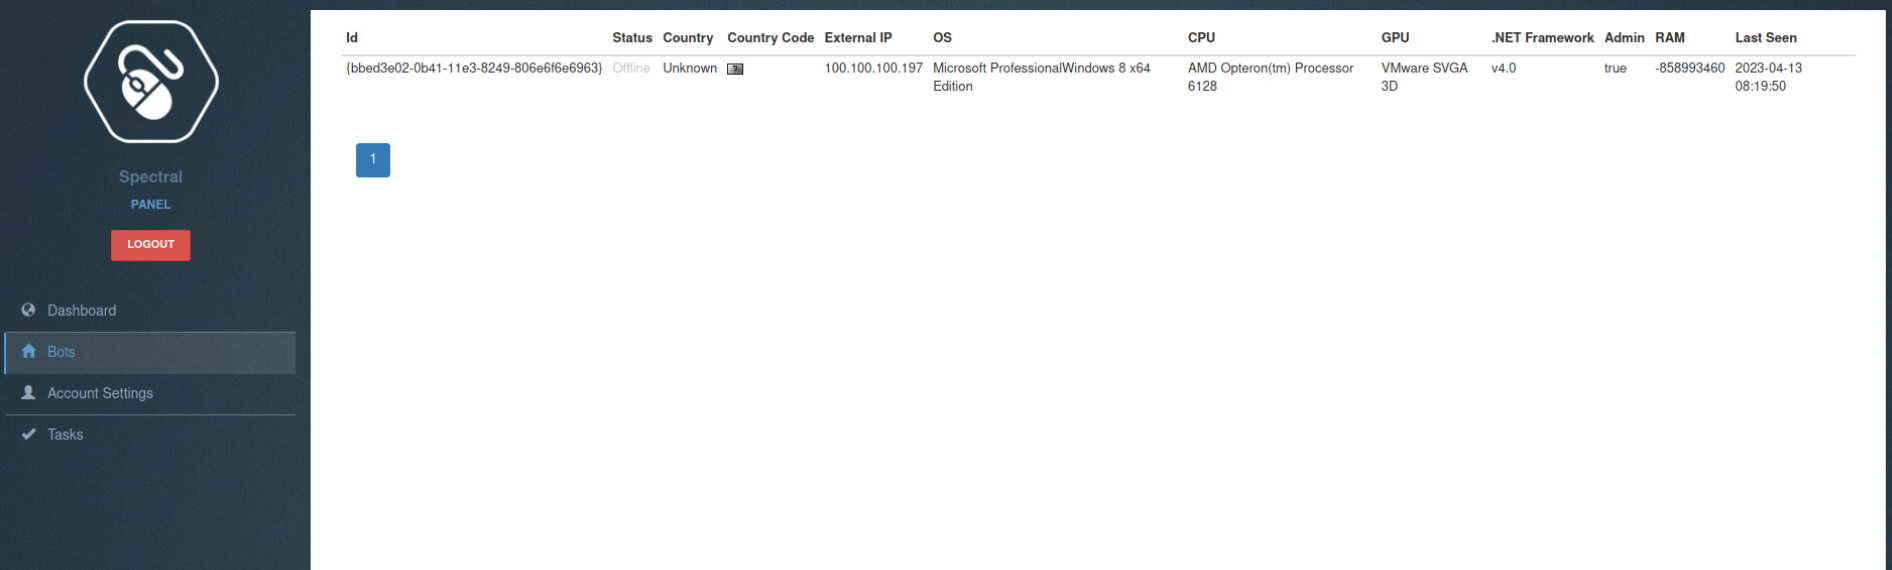
\includegraphics[width=\textwidth,height=0.45\textwidth]{res/fig/uboat-home.png}
        \caption{}
        \label{fig:uboat-home-1}
    \end{subfigure}
    \begin{subfigure}{0.45\textwidth}
        \centering
        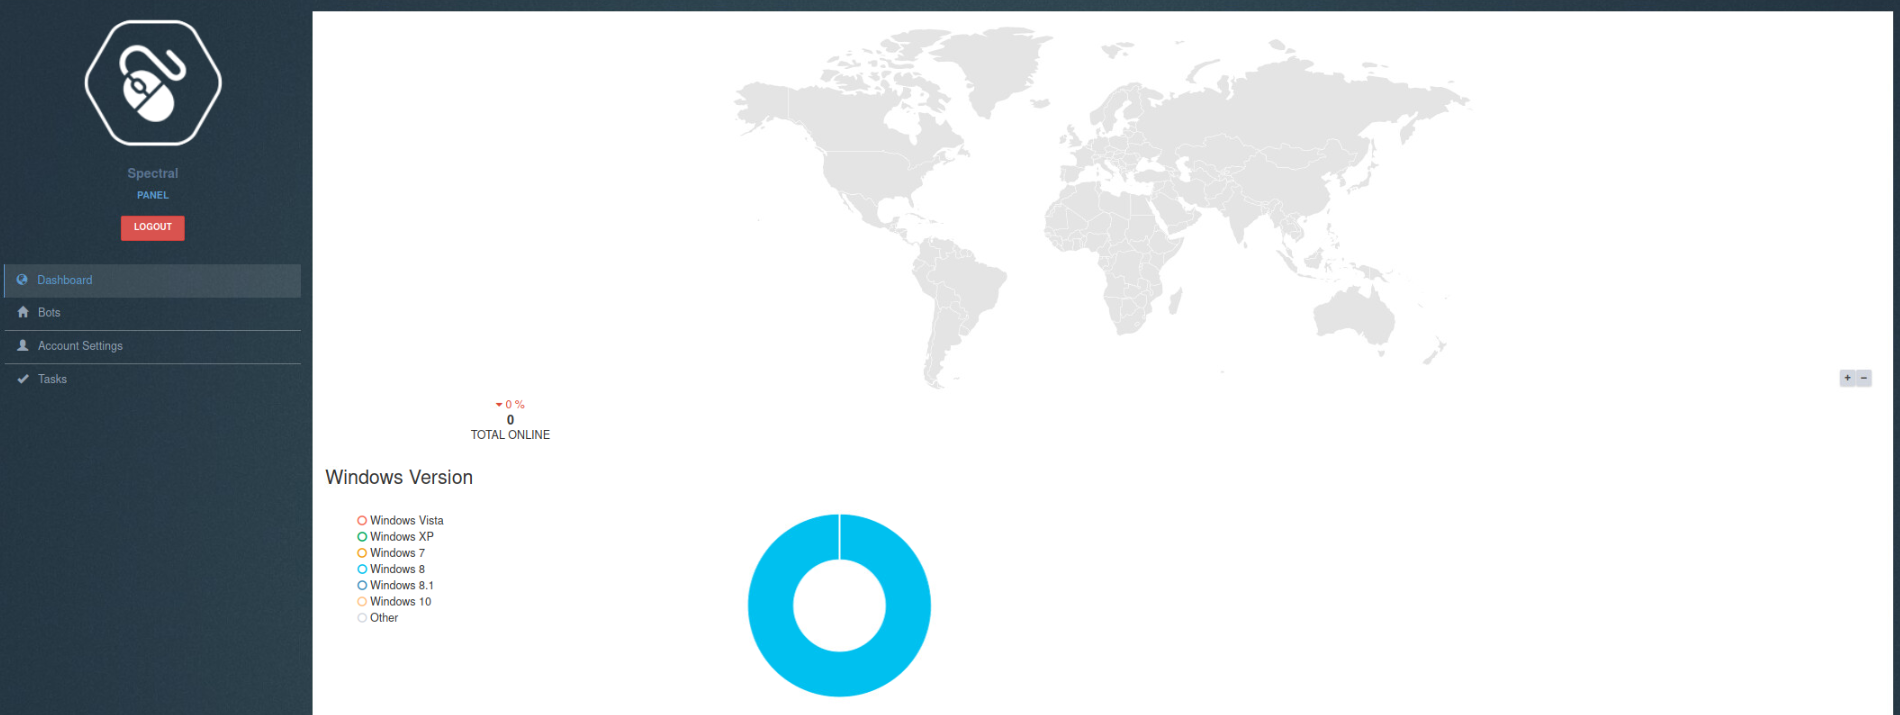
\includegraphics[width=\textwidth,height=0.45\textwidth]{res/fig/uboat-map.png}
        \caption{}
        \label{fig:uboat-home-2}
    \end{subfigure}
    \caption{Visualizzazione delle informazioni dei  bot.}
    \label{fig:uboat-home}
\end{figure}

In \Cref{fig:uboat-home-1} si vede l'interfaccia di visualizzazione dei bot che hanno avuto interazioni col server mentre in \Cref{fig:uboat-home-2} è mostrata la pagine web attraverso cui si può controllare la posizione geografica dei bot.

I bot possono essere selezionati per poter eseguire operazioni su di essi, la \Cref{fig:uboat-control} mostra l'interfaccia di comando dei bot attraverso la quale è possibile inoltrare task operazionali.
\begin{figure}[hbtp]
    \centering
    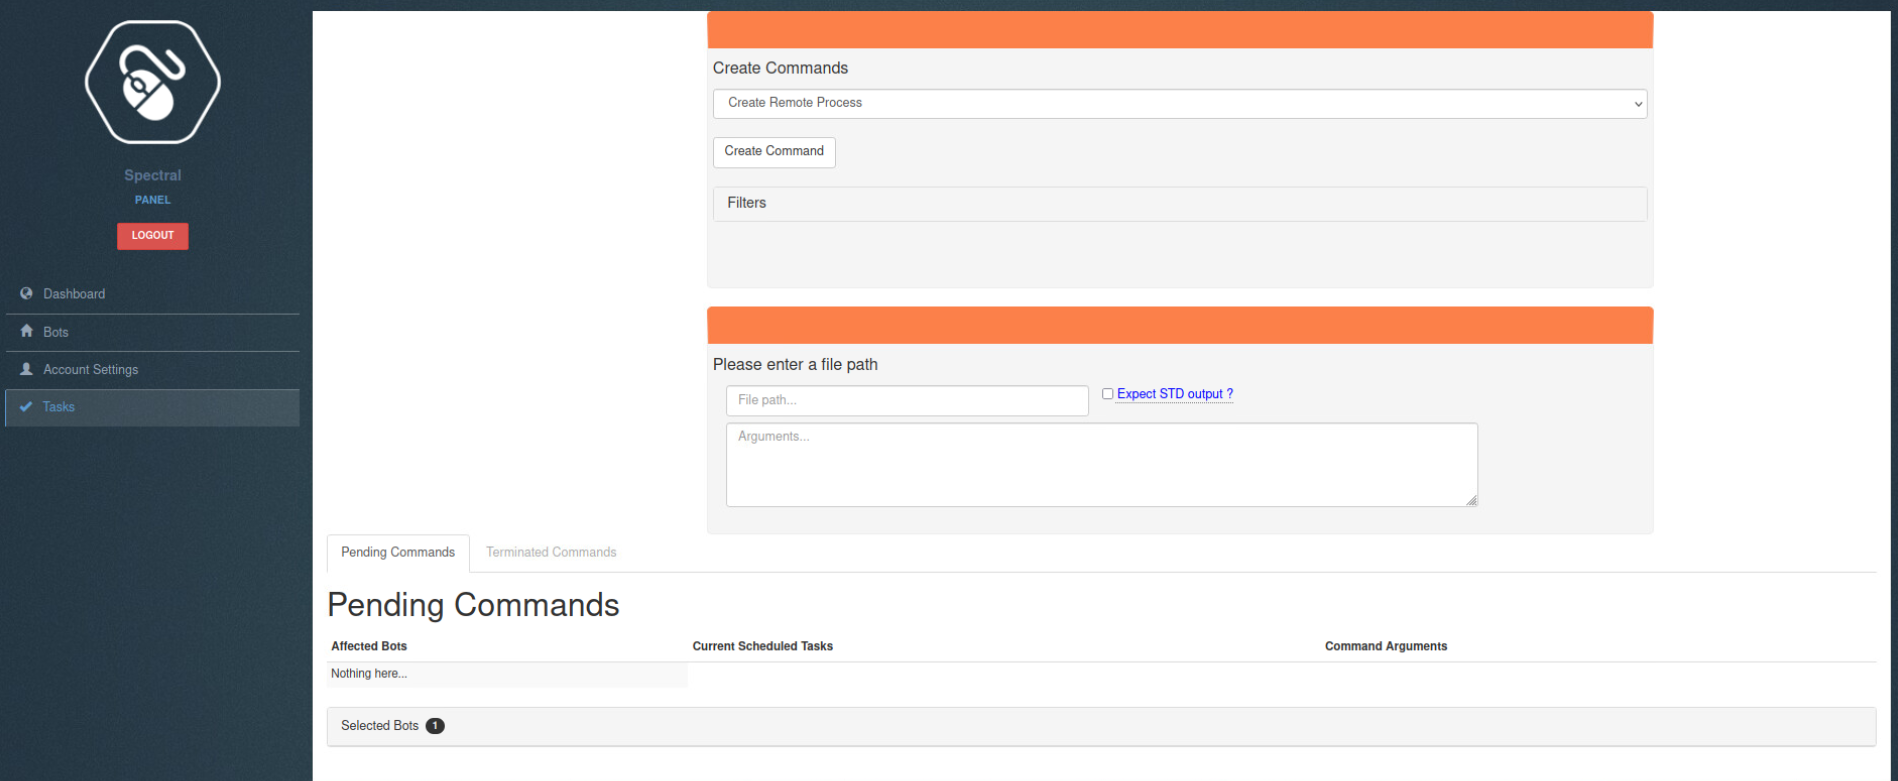
\includegraphics[width=0.45\textwidth]{res/fig/uboat-control.png}
    \caption{Interfaccia di controllo dei bot.}
    \label{fig:uboat-control}
\end{figure}

\section{Dettagli implementativi}

\subsection{Server}
Il C\&C è composto di un web server, cui tecnologia è   a discrezione dell'utente, e di MariaDB, un Database Management System (DBMS) relazionale.
Mantiene le informazioni dei bot, i comandi inseriti ed altre informazioni all'interno del database. Il web server e la relativa interfaccia web sono  raggiungibili attraverso la porta 8080 dell'host che ospita il web server.

Una volta che il server è operativo, aspetta che un bot si metta in contatto con esso.
Il bot comunica con il server attraverso comandi di \textit{Join} o di \textit{Poll} attraverso richieste HTTP. Il primo viene utilizzato per iniziare la comunicazione col server. Alla ricezione del comando di Join quindi il server controlla che il bot sia presente all'interno del database e nel caso non lo fosse viene aggiunto. Il comando di Poll invece, viene utilizzato per richiedere comandi al server. Questa peculiarità  definisce la botnet come pull-based.
Il server riceve anche comandi contenenti l'esito dei task inoltrati.


Il server inoltre,  mantiene un ulteriore processo in background che esegue codice PHP. Questo   si occupa di gestire l'upload degli screenshot, inviati dai bot attraverso richieste HTTP POST.
\subsection{Payload}
\label{Uboat-dettagli-payload}
Il payload usa librerie di Windows per svolgere i propri task e quindi è eseguibile solo su tale sistema operativo.

All'avvio dell'esecuzione del payload, il Bot crea un thread che ha lo scopo di creare persistenza all'interno della macchina vittima.  Per prima cosa crea una directory all'interno del sistema e vi posiziona all'interno una copia dell'eseguibile. Successivamente inserisce un record all'interno del registro di sistema Windows.
Il registro di sistema di Windows è un database gerarchico che archivia le informazioni, le impostazioni e le configurazioni necessarie per il funzionamento  del sistema operativo Microsoft Windows.
Il record in questione usa la chiave RunOnce all'interno del registro per far sì che il payload venga eseguito ad ogni accesso dell'utente. Infine il thread entra in un loop che si preoccupa di controllare la presenza della copia del payload e della chiave di registro, e nel caso reinserirli.

Una  volta creato il thread, esegue l'inizializzazione delle \textit{socket} e degli handler dei comandi che riceverà dal server.

In seguito invia un comando di \textit{Join} al server attraverso HTTP, in cui all'interno inserisce le informazioni della macchina infetta ed in particolare:
\begin{itemize}
    \item Version di Windows installata;
    \item Modello di CPU;
    \item Versione di framework .NET\footnote{ambiente di esecuzione realtime della piattaforma .NET \cite{netframework}.} installata;
    \item Quantità di RAM;
    \item Se l'utente ha diritti di amministratore;
    \item Identificativo Hardware (HWID) associato al dispositivo.
\end{itemize}
In fine entra in un loop che si occupa di gestire la comunicazione col server e tutte le fasi operazionali di cui è incaricato.
Entrando nei dettagli del loop, invia periodicamente un comando di Poll  a cui master risponde all'occorrenza con il prossimo comando da eseguire. Quando il comando viene ricevuto, ne esegue il parsing e nel caso sia un comando riconosciuto esegue l'handler ad esso associato. Infine attenda una quantità di tempo preimpostata prima di ripetere il ciclo e quindi di rieffettuare il polling verso il server.

\medskip
Un comando è composto di tre campi: identificativo, tipo e dati.
Il campo dei dati è utilizzato per passare parametri aggiuntivi al bot o per l'inoltro di risultati di operazioni al server.

%descrizione parser
Nella sezione di codice \ref{listing-uboat1} si può osservare un esempio di handler dei comandi. L'handler in esame è  responsabile di inoltrare uno screenshot al server.  In primo luogo analizza i dati aggiuntivi passati come parametro per estrapolare la porta a cui è associato il processo incaricato di gestire gli upload. In seguito viene eseguito lo screenshot e inoltrato al server sulla porta specificata. Infine invia l'esito del task al server con un ulteriore comando.




%aggiunta descrizione creazione comando

\medskip

L'inoltro di un comando è preceduto da una fase di offuscamento di seguito descritta: 
\begin{enumerate}
    \item Generazione di una chiave di 32 Byte generata con algoritmo pseudocasuale;
    \item Il comando, compreso dei tre campi precedentemente descritti, viene combinato con la chiave attraverso XOR.
    \item Il comando e la chiave vengono codificati in Url \textit{charset}.
    \item La chiave viene inserita negli header della richiesta POST mentre il comando nel \textit{body}.
\end{enumerate}

\lstset{numbers=left,tabsize=2}
\begin{lstlisting}[float,floatplacement=H,caption={Esempio di handler di comandi.},captionpos=b,label={listing-uboat1}]{numbers=left}
void ScreenshotParser(int commandId, int commandType, char* data)
{
	int len;
	char** splitResults = SplitString(data, "@", &len, false);
	unsigned short port = (unsigned short)strtoul(splitResults[1], NULL, 0);

	int length;
	char* scr = CaptureScreenshot(&length);

	bool result = SendScreenshot(splitResults[0], port, scr, length,
            GetBotId());
	FreeSplitStringBuffer(splitResults, len);

	char* command = CreateCommand(commandId, commandType,
            result ? "Success" : "Fail", result ? 7 : 4);
	FreeScreenshot(scr);
	char* response = SendCommandWithDecodedResponse(command);
	FreeDecodedResponse(response);
}
\end{lstlisting}

\section{Deploy, testing e debug}
Il deploy del server è stato eseguito attraverso containerizzazione del web server e del DBMS. In particolare è stato utilizzato Docker Compose per eseguire contemporaneamente entrambi i container attraverso un unico file di configurazione ed un unico comando.
Questo (\ref{listing-uboat2}) illustra le porte e le directory da mappare, le variabili d'ambiente da utilizzare per la configurazione di MariaDB, nonché altre informazioni pertinenti, come la rete a cui associare i servizi e informazioni di risoluzione dei container.
L'handler delle richieste di upload veniva eseguito dall'interno del container all'occorrenza, eseguendo uno script PHP in background.

\medskip 
Dopo aver configurato l'indirizzo del server  C\&C nel codice sorgente del payload e installato gli strumenti necessari, come il Software Developer Kit (SDK) e i Build Tools, il payload è stato compilato ed eseguito in Visual Studio. Questo ha permesso di utilizzare il \textit{debugger} integrato dell'IDE per analizzare il funzionamento del bot.

\medskip
Prima di procedere con il test della botnet, sono state apportate alcune modifiche al fine di risolvere alcuni dei bug individuati, i quali verranno di seguito descritti:
\begin{itemize}
    \item Le richieste HTTP del server non erano indirizzate verso il corretto percorso di rete (path);
    \item Quando il bot inviava il messaggio di Join al server, le informazioni inserite al suo interno erano posizionate in un ordine differente dall'ordine in cui venivano elaborate dal server. Il server quindi, nel procedere all'inserimento in database dei dati ricevuti, generava un'eccezione, poiché i tipi dei dati inseriti non combaciavano con i tipi dei dati della \textit{query} di inserimento;
    \item Il percorso in cui venivano salvati i risultati del Keylogger, era formattato erroneamente;
    \item Una delle directory in cui venivano salvate delle informazioni non era presente al momento dell'esecuzione e non avendo abbastanza permessi per crearla ne conseguiva il malfunzionamento;
    \item L'inoltro dello screenshot è diviso in due scambi di dati tra server e bot, ma era coordinato male. In particolare vi era un problema di sincronizzazione per via della ricezione non bloccante dei messaggi;
    \item La funzionalità di persistenza, che prevede l'inserimento di un record nel registro di sistema, presentava un bug che causava l'inserimento continuo della chiave nel registro stesso.
\end{itemize}

Una volta sistemati questi bug è stato possibile testare le varie funzionalità operative della botnet:
\begin{itemize}
    \item Esecuzione di processo da remoto con possibilità di aggiungere parametri. La possibilità di aggiungere parametri permette anche di eseguire script, ad esempio, eseguendo un'interprete di comandi e passandogli comandi interpretabili;
    \item Funzionalità DDoS, seppure l'implementazione non sia molto efficiente. Essa infatti consiste di un loop in cui vengono aperte connessioni TCP verso il target per inviare una serie di dati. Per provvedere alla scarsa efficienza della funzionalità built-in, è stato testato un tool di DDoS reperito in Internet, che è stato eseguito per mezzo della funzionalità di esecuzione di processi;
    \item Keylogging, ovvero la capacità di poter estrapolare  dal bot, in forma di dati, le digitazioni da tastiera dell'utente;
    \item Download ed esecuzione di eseguibile. Un dettaglio importante che verrà utilizzato nella fase di rilevazione, è che il bot usa l'\textit{esplora risorse} di Windows per eseguire i file scaricati;
    \item La funzionalità di update del bot è molto simile al \textit{download and execute} già visto. Il bot esegue il download del nuovo payload, lo esegue ed in seguito termina la propria esecuzione per lasciare spazio alla versione aggiornata;
    \item Capacità di inviare una richiesta HTTP ad un sito web target per controllare che sia operativo. Ritorna esito positivo solo in caso la risposta HTTP abbia codice 200.
\end{itemize}





\begin{lstlisting}[firstnumber=1,floatplacement=H,caption={File di configurazione docker compose.},captionpos=b,label={listing-uboat2}]{numbers=left}
version: '3'

services:
  webserver:
    image: uboat-webserver
    build: .
    ports:
      - "80:80"
      - "25019:25019"
    volumes:
      - ./public:/var/www/html
      - ./src:/var/www/src
      - ./logs:/var/www/src/logs
      - ./screenshots:/var/www/src/screenshots
    links:
      - mysql
    networks:
      - vlan

  mysql:
    image: mariadb:10.1
    ports:
      - "3306:3306"
    volumes:
      - ./container/mysql/var/lib/mysql:/var/lib/mysql
      - ./container/sqlFiles:/home/sqlFiles
    environment:
      - MYSQL_DATABASE=uboat
      - MYSQL_USER=uboat
      - MYSQL_PASSWORD=uboat
      - MYSQL_ROOT_PASSWORD=root
    networks:
      - vlan

networks:
  vlan:
\end{lstlisting}

\section{Rilevazioni con IDS}
%lua scripting su richieste http per deoffuscare
\subsection{Network based IDS}
L'invio periodo delle richieste di Poll da parte del bot non rilevano niente  di sospetto se non che le richieste sono destinate a indirizzi IP e non a hostname, cosa abbastanza insolita in un contesto normale.

Se l'indirizzo IP del server fosse noto come un indirizzo IP malevolo e fosse inserito all'interno di liste di IP considerati pericolosi, gli IDS  potrebbero rilevare il traffico di rete sfruttando queste liste. 

\medskip

La funzionalità di download and execute del server viene rilevata dagli IDS. In particolare è stato segnalato il download di un eseguibile con pochi header, tipico di file Stager, e che il download è avvenuto verso un indirizzo IP non specificandone l'hostname. Inoltre rileva anche la presenza della keyword 'isDebuggerPresent', tipicamente utilizzata all'interno di malware per applicare restrizioni di anti-debugging.
In caso di download di file malevolo noto come un malware, Strelka si preoccuperebbe di segnalarne l'identificazione

La funzionalità di update porta agli stessi risultati in quanto il funzionamento è quasi identico.

\medskip

Il controllo dello stato di un sito web non ha ovviamente rilevato nulla in quanto è basato su una semplice richiesta HTTP, ed essendo questo un protocollo comune in rete.

\medskip
L'esecuzione di un processo da remoto, l'estrapolazione di screenshot e il keylogging non sono stati segnalati, in quanto il loro comportamento malevolo avviene principalmente  sull'host piuttosto che sulla rete.

\medskip

L'attacco DDoS non ha portato a segnalazioni.

\medskip
Lo scambio di comandi tra bot e server non è segnalato come malevolo in quanto non erano presenti regole di matching mirate alla rilevazione di UBoat, oltre al fatto che i comandi all'interno del corpo del messaggio sono offuscati.
Un modo per poter rilevare la presenza di UBoat potrebbe essere sfruttare le capacità di LUA scripting di Suricata per deoffuscare il messaggio, in congiunta con l'inserimento di regole specifiche basate sul matching del formato dei messaggi di UBoat.

\medskip
In aggiunta alle funzionalità della botnet è stata sfrutta la capacità di instaurare una reverse-shell sfruttando le capacità built-in, per analizzare se gli IDS l'avrebbero segnalata.
In \Cref{fig:uboat-reverseshell1} si può osservare il comando composto\footnote{formulato per testare anche la capacità di eseguire più comandi in un solo messaggio.} utilizzato per creare una reverse shell sfruttando Nmap \cite{nmap}. Il server apre una porta e rimane in ascolto mentre il bot, attraverso Nmap,  esegue un comando e ne redirige l'input e l'output verso la porta aperta del server.

A scopo di test, Nmap è stato installato sulla macchina vittima, in un contesto reale si potrebbe sfruttare la capacità di composizione dei comandi (osservabile in \Cref{fig:uboat-reverseshell1}) per eseguirne prima il download e poi l'esecuzione.

In \Cref{fig:uboat-reverseshell2} si può osservare il successo effettivo dell'operazione di reverse-shell, che tuttavia, l'IDS non ha rilevato.

\begin{figure}
    \centering
    \begin{subfigure}{0.4\textwidth}
    \centering
    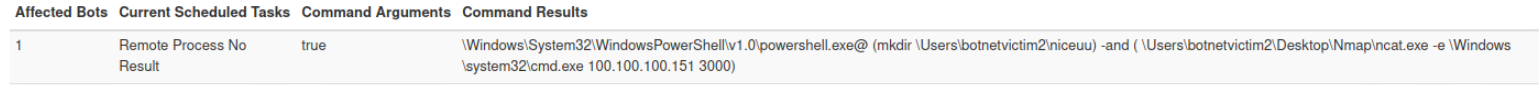
\includegraphics[width=\textwidth]{res/fig/reverse-shell1.png}
    \caption{Comando per la creazione di una reverse-shell.}
    \label{fig:uboat-reverseshell1}
    \end{subfigure}
    \hfill
    \begin{subfigure}{0.4\textwidth}
    \centering
    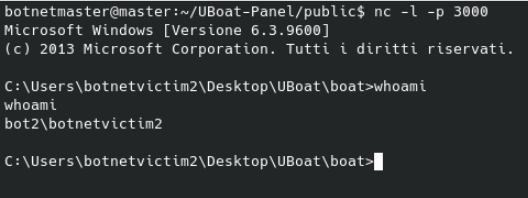
\includegraphics[width=\textwidth]{res/fig/reverse-shell2.png}
    \caption{Shell collegata al bot.}
    \label{fig:uboat-reverseshell2}
    \end{subfigure}
    \caption{}
    \label{fif:uboat-reverseshell}
\end{figure}

\subsection{Host based IDS}
Combinando Sysmon con Wazuh è stato possibile sfruttare a pieno le funzionalità di HIDS che offre come Agent. Attraverso il set di regole di Wazuh, molto vasto e completo, è stato possibile identificare azioni potenzialmente malevole come la creazione di un record all'interno del registro di sistema o la creazione di file in zone delicate. Per sfruttare a pieno le capacità di rilevazione di Wazuh, e testare a pieno le capacità di rilevazione signature-based, sono state create delle regole Wazuh atte ad identificare UBoat.
Queste regole sono basate sulle principali caratteristiche di UBoat descritte in precedenza, e su altri dettagli implementativi.
\lstset{float,floatplacement=H,frame=none,tabsize=1,numbers=none}

Attraverso l'aggiunta delle seguenti configurazioni a quelle dell'agent sulla macchina target è stato possibile monitorare le connessioni aperte e  directory specifiche. In caso di cambiamenti, come aggiunta o rimozione di file, all'interno di una delle directory monitorate, verrà generato un evento.
\lstset{xleftmargin=1cm}
\begin{lstlisting}
<ossec_config>
    <syscheck>
        <disabled>no</disabled>
        <directories realtime="yes">path a directory 
            da monitorare</directories>
        ...
    </syscheck>
    <localfile>
        <log_format>full_command</log_format>
        <command>netstat -n</command>
        <alias>netstat command</alias>
        <frequency>60</frequency>
        ...
    </localfile>
    ...
</ossec_config>
\end{lstlisting}

Di seguito analizzeremo le regole utilizzate per identificare le varie funzionalità operative della botnet.
Le regole 100013 e 100014 sono utilizzate per identificare connessioni verso l'indirizzo IP della botnet, sfruttando la lista delle connessioni aperte inviate dall'agent. Le regole 100015 e 100016 sono state realizzate per cancellare il rumore creato dall'esecuzione del comando utilizzato per identificare le connessioni di rete sulla macchina monitorata.
\begin{lstlisting}
<group name="ossec">
    <rule id="100013" level="0">
        <if_group>ossec</if_group>
        <match>netstat</match>
        <description>netstat command execution</description>
    </rule>
    <rule id="100014" level="12">
        <if_sid>100013</if_sid>
        <match>100.100.100.151</match>
        <description>Botnet - connection to botnet server</description>
    </rule>
    <rule id="100015" level="0">
        <if_sid>92052</if_sid>
        <field name="win.eventdata.parentImage">wazuh-agent.exe</field>
        <description>agent check command execution</description>
    </rule>
    <rule id="100016" level="0">
        <if_sid>92032</if_sid>
        <field name="win.eventdata.parentImage">cmd.exe</field>
        <field name="win.eventdata.image">NETSTAT.EXE</field>
        <description>agent check command execution</description>
    </rule>
</group>
\end{lstlisting}

La regola 100007 sfrutta la capacità di monitorare directory designate precedentemente descritta, e genera un allarme nel caso nella particolare directory sia inserito un file eseguibile denominato 'filename.exe'. In questo caso si sfrutta l'hardcoding del nome del file per identificare la botnet.
\begin{lstlisting}
<group name="syscheck">
    <rule id="100007" level="12">
        <if_sid>554</if_sid>
        <regex>foldername\\\\filename.exe\.*added</regex>
        <description>Botnet - malware file creation for persistance 
            </description>
    </rule>
</group>
\end{lstlisting}

Di seguito verranno le analizzate le regole che sono state realizzate sfruttando le funzionalità di generazione eventi di Sysmon.
Le regole 100002 e 100003 sono utilizzate per allertare che è stata inserita una determinata chiave di registro in una specifica posizione del registro di sistema. 

\begin{lstlisting}
<rule id="100002" level="0">
    <if_group>sysmon</if_group>
    <match>Registry value set</match>
    <description>Registry value set</description>
    <options>no_log</options>
</rule>
<rule id="100003" level="12">
    <if_sid>100002</if_sid>
    <field name="win.eventdata.targetObject">\\\\RunOnce\\
        \\RegKey</field>
    <field name="win.eventdata.details">\\\\AppData\\\\Roaming\\
        \\FolderName\\\\FileName.exe</field>
    <description>Botnet - reg key insertion</description>
</rule>

\end{lstlisting}

La regola 100017 fa riferimento all'esecuzione del payload ormai persistenze all'interno del computer della vittima. Grazie al meccanismo precedentemente analizzato, sfrutta la chiave di registro 'RunOnce' per avviare l'esecuzione del bot all'accesso dell'utente, e questa regola si basa su questa azione.

\begin{lstlisting}
    
<rule id="100017" level="12">
    <if_group>sysmon</if_group>
    <match>Process create</match>
    <field name="win.eventdata.image">FileName.exe</field>
    <description>Botnet - botnet execution</description>
</rule>
\end{lstlisting}

La regola 100018 ha fine  analogo a quello della regola 100014, ovvero la rilevazione di una connessione col C\&C noto. Tuttavia mentre la prima fa affidamento sul risultato dell'esecuzione di un comando sull'agent, la seconda sfrutta gli eventi di Sysmon per generare un allarme.

\begin{lstlisting}
<rule id="100018" level="12">
    <if_group>sysmon</if_group>
    <match>Network connection detected</match>
    <field name="win.eventdata.destinationIp">100.100.100.151</field>
    <description>Botnet - connection to botnet server initiated
        </description>
</rule>
\end{lstlisting}

La regola 100019 sfrutta la rilevazione della regola 100018 in combinazione con la porta nota dell'handler degli upload per segnalare l'estrapolazione di screenshot.

\begin{lstlisting}  
<rule id="100019" level="12">
    <if_sid>100018</if_sid>
    <field name="win.eventdata.destinationPort">25019</field>
    <description>Botnet - screenshot exfiltration</description>
</rule>
\end{lstlisting}

Le regole 100020 e 100021 sono utilizzate in combinazione per rilevare uno spike del numero di connessioni in uscita dall'host monitorato e  segnalare quindi l'origine di un possibile attacco DoS.
\begin{lstlisting}
<rule id="100020" level="5">
    <if_group>sysmon</if_group>
    <field name="win.eventdata.sourceIp">100.100.100.197</field>
    <field name="win.eventdata.destinationIp" negate="yes">
        100.100.100.151</field>
    <description>connection initiated from host</description>
    <options>no_log</options>
</rule>
<rule id="100021" level="12" frequency="200" timeframe="10">
    <if_matched_sid>100020</if_matched_sid>
    <description>Possible DoS attack originated from host</description>
</rule>
\end{lstlisting}

\medskip
Le regole 100022 e 100023 mirano ad identificare il download e l'esecuzione attraverso l'explorer manager, di file malevoli. Ancora una volta si sfrutta la conoscenza del sorgente del malware e il pattern matching con parole chiave.
\begin{lstlisting}
<rule id="100022" level="12">
    <if_sid>92213</if_sid>
    <field name="win.eventdata.targetFilename">BOTNET</field>
    <description>Botnet - Downloaded executable</description>
</rule>
<rule id="100023" level="12">
    <if_sid>61640</if_sid>
    <field name="win.eventdata.image">explorer.exe</field>
    <field name="win.eventdata.commandLine">BOTNET</field>
    <description>Botnet - execution of downloaded file</description>
</rule>
\end{lstlisting}

\medskip

Concludiamo lo studio di UBoat con una carrellata delle segnalazioni effettuate da Wazuh in seguito all'aggiunta delle regole e configurazioni presentate.
\begin{figure}[hbtp]
    \centering
    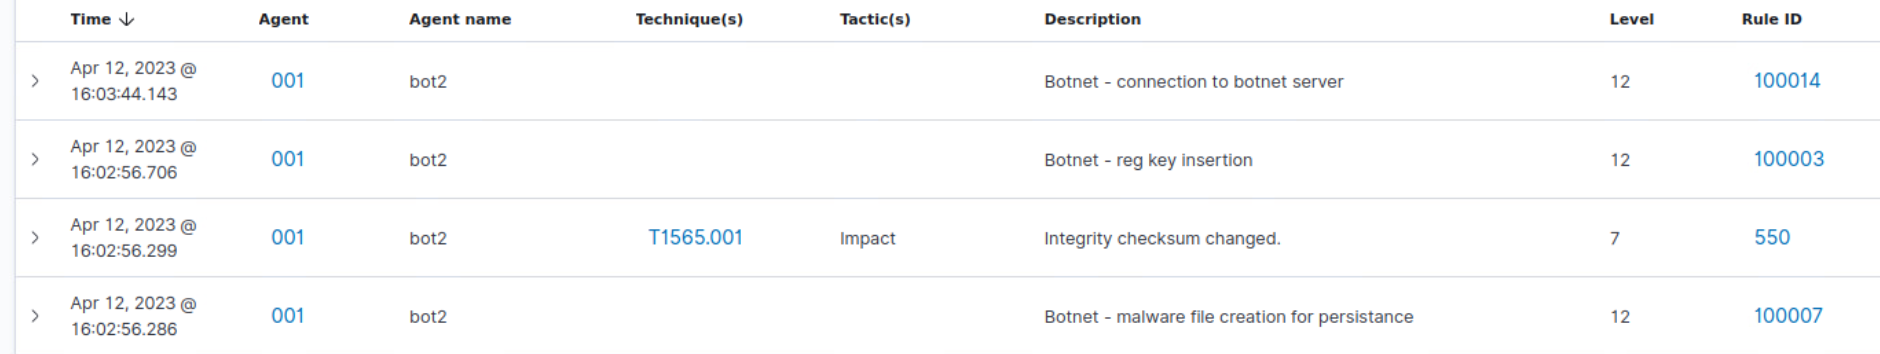
\includegraphics[width=\textwidth]{res/fig/uboat-result1.png}
    \caption{Segnalazioni all'esecuzione del payload.}
\end{figure}
\begin{figure}[hbtp]
    \centering
    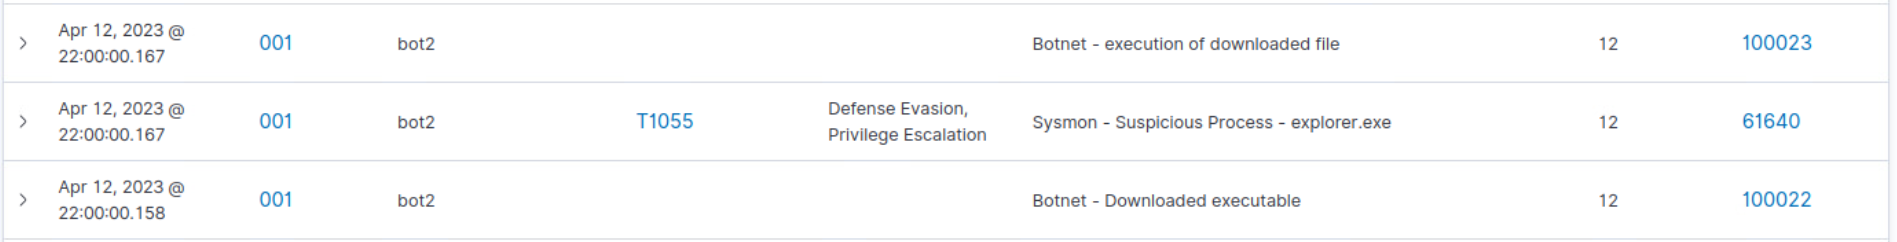
\includegraphics[width=\textwidth]{res/fig/uboat-result2.png}
    \caption{Segnalazioni in seguito alla funzionalità di Download and Execute.}
\end{figure}
\begin{figure}[hbtp]
    \centering
    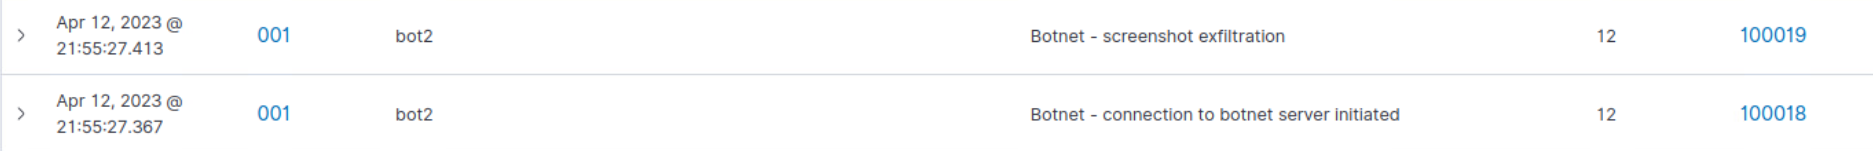
\includegraphics[width=\textwidth]{res/fig/uboat-result3.png}
    \caption{Segnalazioni in seguito all'estrapolazione di screenshot.}
\end{figure}
\begin{figure}[hbtp]
    \centering
    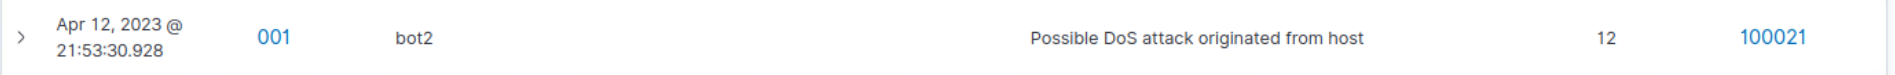
\includegraphics[width=\textwidth]{res/fig/uboat-result4.png}
    \caption{Segnalazioni in seguito all'attacco DoS.}
\end{figure}
\begin{figure}[hbtp]
    \centering
    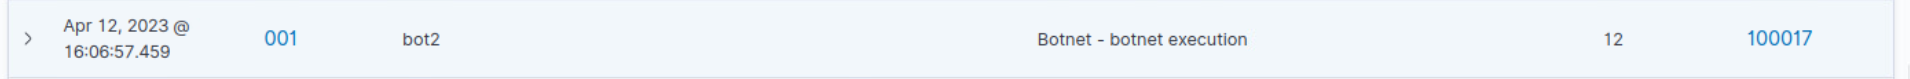
\includegraphics[width=\textwidth]{res/fig/uboat-result5.png}
    \caption{Segnalazioni in merito l'esecuzione all'accesso dell'utente.}
\end{figure}


\chapter{Analisi e altri possibili approcci fingerprint based}

Nei capitoli precedenti è stato osservato  come l'utilizzo di un agente  e delle relative funzionalità di HIDS possano essere utilizzate per  aumentare il panorama di caratteristiche analizzabili di un sistema e incrementarne di conseguenza la sicurezza.

Dalle analisi condotte sulle due botnet, emerge che sono stati utilizzati principalmente software IDS che utilizzino strumenti di rilevazione basati su tecniche di pattern matching, prediligendo quindi l'approccio fingerprint based.
Come osservato nel \Cref{IDS}, gli approcci fingerprint based funzionano molto bene per malware e attività malevole per cui esista già una firma identificativa al momento della rilevazione. Nello studio  effettuato su UBoat (\Cref{uboat}) si può osservare come le regole create per l'identificazione della botnet siano basate su caratteristiche peculiari del software analizzato. Piccole variazioni o l'offuscamento all'interno del codice del  payload, potrebbero rendere parte delle regole di rilevazione create inefficienti verso la nuova versione del software malevolo. Ad esempio, se il botmaster distribuisse una nuova versione del payload, che durante la fase operativa di instaurazione della persistenza inserisce una copia dell'eseguibile nel sistema con un nome o una posizione differenti da quelle specificate, si potrebbero perdere gli allarmi relativi a tale evento.
Complicazioni aggiuntive come la cifratura del traffico di rete e tecniche di \textit{detection evasion} possono rendere ancora più ardua la rilevazione.
Inoltre come già precedentemente osservato, tale approccio non può essere applicato in caso di malware zero-day. Per cercare di ovviare a queste problematiche i ricercatori e vendor di sistemi di sicurezza informatici, cercano di tenere i database di fingerprint  il più aggiornati possibile oltre a ricercare nuove tecniche principalmente basati su rilevazioni di anomalie.

\medskip
Tra le tecniche e le possibilità di rilevazione  fingerprint based analizzate, che sarebbe possibile integrare facilmente all'interno dell'infrastruttura di testing sviluppata, vi sono:
\begin{itemize}
    \item Yara rules;
    \item Integrazione con virus engine;
    \item API calls.
\end{itemize}

\smallskip
Yara \cite{yara} è un tool utilizzato per ricercare e classificare malware. Attraverso Yara è possibile creare descrizioni, anche dette regole, basate su pattern testuali o binari.
Le YARA rule sono scritte in una sintassi specifica che permette di definire una serie di criteri di ricerca per individuare un determinato oggetto o comportamento. Ogni regola YARA è composta da tre sezioni principali:
\begin{description}
    \item [Meta] Contiene il nome della regola e altre informazioni, come l'autore, la data di creazione e la descrizione della regola stessa.
    \item [Strings] Contiene i pattern che vengono utilizzati all'interno della sezione Condition.
    \item [Condition] La parte centrale della regola che definisce il criterio di ricerca da applicare. La condizione è composa di un'espressione booleana e di stringhe su cui eseguire il match.
\end{description}

Un esempio di Yara rule è il seguente \cite{yaraexample}:
\begin{lstlisting}[caption={Esempio di Yara rule.},captionpos=b,frame=single]
rule silent_banker : banker
{
    meta:
        description = "This is just an example"
        threat_level = 3
        in_the_wild = true

    strings:
        $a = {6A 40 68 00 30 00 00 6A 14 8D 91}
        $b = {8D 4D B0 2B C1 83 C0 27 99 6A 4E 59 F7 F9}
        $c = "UVODFRYSIHLNWPEJXQZAKCBGMT"

    condition:
        $a or $b or $c
}
\end{lstlisting}


All'analisi di un file, la regola in esempio, andrà alla ricerca dei pattern binari e testuali elencati nella sezione Strings e nel caso almeno uno venisse trovato la regola darebbe esito positivo e il file sarebbe etichettato come \textit{silent\_banker}.
\smallskip
Le Yara rule sono utilizzate all'interno di Strelka in Security Onion per la ricerca di file malevoli all'interno del traffico di rete. Questo approccio può essere importato all'interno dell'host da monitorare. Attraverso Wazuh, per esempio, è possibile integrare Yara con il modulo di File Integrity Monitoring dell'agent. Così facendo, ogni volta che viene modificato un file monitorato Yara effettuerà una scansione su di esso alla ricerca di file malevoli sfruttando le Yara rule.

\medskip
%integrazione con altri virus engine
%api call stuff
%leggere paper per altri approcci ids per vedere se c'è qualcosa di interessante
%behavior baased IDS

%In questo modo il server può ricevere informazioni ed eventi da un infinita lista di possibili sorgenti.

Per aumentare ulteriormente la sicurezza degli end-point è possibile integrare sistemi antivirus o simili, sfruttando le capacità di inoltro dei log degli agent o di altri software.  Wazuh ad esempio, all'interno della propria documentazione cita ClamAV \cite{clamav} come possibile alternativa open source di software antivirus multi piattaforma, basato su fingerprint. Esso è in grado di supportare diversi tipi di signature per analizzare molteplici formati di file, compresi archivi ed email.

Su un sistema Windows può essere utile sfruttare i log di Windows Defender\footnote{antivirus installato di default all'interno dei sistemi operativi Windows.} per avere visibilità delle infezioni rilevate da esso o per analizzare i risultati di possibili scansioni effettuate.

Un'ultima menzione è la possibilità di integrazione del modulo di File Integrity Monitoring degli agent Wazuh con il servizio VirusTotal \cite{virustotal}. VirusTotal è un sistema che sfrutta più di 70 antivirus/scanner e molteplici liste di domini/IP malevoli, per eseguire l'analisi di file online direttamente dal portale web del servizio. Esso offre inoltre un API utilizzabile per sfruttare il servizio programmaticamente. Grazie all'integrazione con Wazuh, quando l'agente segnala un cambiamento, una creazione o una cancellazione di un file, il server  utilizza l'API di VirusTotal per inoltrare l'hash del file e ricevere i risultati dell'analisi da esso effettuata.

In conclusione, questi sono solo alcuni dei potenti esempi di integrazione che è possibile effettuare per aumentare ulteriormente l'analisi su un sistema. Il vasto mercato dei sistemi di sicurezza lascia un'ampia scelta all'amministrazione della sicurezza, permettendo di personalizzare ulteriormente il livello di protezione del sistema.


\medskip

%api hooking poi conclusione
 
Per quanto riguarda le API call invece, si è voluto testare  uno dei meccanismi utilizzato da molti  Endpoint Detection and Response (EDR) e antivirus, per il monitoraggio di  processi in real-time alla ricerca di comportamenti malevoli.  
La tecnica in questione è chiamata API hooking. 

L'API hooking  consente di monitorare e intercettare le chiamate ad una o più API call di un sistema operativo o di un'applicazione, per modificare o estendere il loro comportamento. In pratica, l'API hooking consente di intercettare la comunicazione tra un'applicazione e il sistema operativo, permettendo di monitorare e modificare il comportamento dell'applicazione o del sistema operativo stesso, ad esempio per rilevare e prevenire attacchi informatici.

L'idea di fondo era utilizzare tale tecnica per monitorare le chiamate di sistema di un software alla ricerca di pattern nell'ordine o insieme di chiamate effettuate. 


%spiegare api hooking
Entrando nei dettagli, un possibile  esempio di hooking di chiamata di  funzione in un processo a 32 bit può essere il seguente \cite{hooking1,hooking2}:
\begin{enumerate}
    \item Si estrae l'indirizzo in memoria della funzione di cui si vuole eseguire l'hook;
    \item Vengono salvati i primi 5 byte  della funzione e messi da parte;
    \item Si crea la funzione a cui passerà il controllo quando la funzione di cui si vuole eseguire l'hook viene chiamata, che chiameremo \textit{HookedFunction}. Prima che questa finisca la propria esecuzione, riscriverà i byte  precedentemente salvati al loro posto, per poi eseguire la funzione originale;
    \item Si estrae l'indirizzo in memoria della HookedFunction;
    \item Si sovrascrivono i primi 6 byte della funzione originale con gli opcode di  jump all'indirizzo della HookedFunction.
\end{enumerate}

Questo è il modo più banale di eseguire tale operazione, in quanto ad ogni esecuzione della funzione di cui si esegue l'hook i 6 byte di partenza vengono sovrascritti più volte. Un implementazione più efficiente può essere ottenuta sfruttando i cosiddetti \textit{trampolini}. Un trampolino è una funzione che esegue quanto segue \cite{hooking2}:
\begin{enumerate}
    \item Esegue i byte originali precedentemente salvati della funzione di cui è eseguito l'hook;
    \item Salta all'interno del codice della funzione originaria, dopo l'istruzione di jump inserita manualmente.
\end{enumerate}

Tuttavia tale operazione richiede la gestione del caso in cui la sovrascrittura dei 5 byte iniziali dovessero rompere la sintassi della restante porzione di funzione.

Comunque in entrambi i casi, quando la funzione da monitorare viene eseguita, il controllo passerà alla funzione da noi definita per poi tornare ad eseguire la funzione originale.

Le cose sono però più complicate in processi a 64 bit, dato che le funzioni potrebbero essere posizionate tra loro troppo distanti per far si che siano raggiungibili con un jump relativo a 32 bit. Dato che non esistono jump relativi a 64 bit, si potrebbe pensare di usare un jump assoluto ad un indirizzo di memoria preciso a 64 bit.  Tuttavia tale salto richiede almeno 13 byte di opcode, e quindi tale approccio non sarebbe utilizzabile per funzioni che abbiano meno di 13 byte.

Per risolvere questo problema si può eseguire un salto relativo a 32 bit, che richiede 5 byte di opcode, ad una porzione di codice allocata in  vicinanza (così che sia raggiungibile con un salto relativo) e quindi eseguire il jump assoluto all'indirizzo della HookedFunction.

\smallskip


Wazuh offre la possibilità di monitoraggio di API call su Linux sfruttando l'integrazione con l'Audit System del sistema operativo. Tuttavia, dato che la botnet su cui si sarebbe voluto effettuare il test (UBoat) può eseguire solo su Windows è stato ricercato un software alternativo che servisse allo scopo.

Inizialmente è stato utilizzato WinAPIOverride \cite{winapioverride}, un tool di monitoraggio e hooking di API call per processi a 32 e 64 bit.
Questo offre anche un tool per l'estrazione di tutte le API call effettuate da un software, così che risulti più facile estrarne una possibile fingerprint per i nostri scopi.
A basso livello esso utilizza un Kernel driver rendendo quindi possibile intercettare ogni chiamata di sistema senza dover iniettare codice in applicativo.
Specificando quali API call si desiderasse monitorare e caricando un DLL contenenti le strutture dati con le funzioni sui cui eseguire l'hook e le funzioni a cui ridirigerle, WinAPIOverride si preoccupava di eseguire l'hooking.
All'interno della sezione di codice \ref{winapioverride} è possibile vedere un esempio di struttura dati utilizzata in cui viene specificata l'API call sul quale eseguire l'hook, in questo caso Sleep della libreria kernel32.dll, e funzione definita dall'utente con relativi parametri all'occorrenza.
\lstset{xleftmargin=0cm}
\begin{lstlisting}[frame=single,caption={esempio di struttura dati per hook in WinAPIOverride.},captionpos=b,label={winapioverride}]
STRUCT_FAKE_API_WITH_USERPARAM pArrayAfterAPICall[] =
{    
	{_T("kernel32.dll"),_T("Sleep"),(FARPROC)MyFunction,
            StackSizeOf(DWORD) ,0,0},
	{_T(""),_T(""),NULL,0,0,0}
};
...
\end{lstlisting}

Seppure il programma funzionasse correttamente, la licenza gratuita del tool non permette l'utilizzo su macchina virtuale. Per questo motivo è stato deciso di implementare un piccolo prototipo d'esempio senza l'ausilio di strumenti di terze parti, che sarebbe quindi potuto essere testato su macchina virtuale. Il prototipo è stato tenuto il più semplice possibile in quanto il fine ultimo era il consolidamento di quanto appreso riguardo la tecnica di hooking.
Lo scopo del prototipo è intercettare le API call di un  processo in esecuzione e di inviare un log al Windows Event Log System per notificarne l'accaduto, così che l'agente Wazuh potesse inviare tale log al Server per ulteriore analisi e intrusion detection.

\medskip
%spiegare DLL injetction
%foto prototipo 
Senza il supporto del tool era necessario trovare un modo per poter eseguire il codice, necessario per svolgere le attività di hooking, all'interno del processo da monitorare.
Per fare ciò è stato eseguita una tecnica chiamata DLL injection. Vi sono molti modi per effettuare ciò.
La tecnica utilizzata consiste nel forzare un processo ad eseguire un thread, che è incaricato di caricare  all'interno del contesto del processo una DLL \cite{dllinjection}. Il caricamento di una DLL comporta, tra le cose, l'esecuzione nel contesto del processo del codice contenuto all'interno del \textit{DllMain} della libreria. 

Ricapitolando quindi, inserendo  il codice responsabile dell'hooking all'interno della DLL è possibile eseguirlo attraverso DLL injection all'interno del processo così monitorato.

Entrando nei dettagli, l'implementazione ci compone dei seguenti punti:
\begin{enumerate}
    \item Si ottiene l'handle del processo che si desidera monitorare;
    \item Si alloca memoria all'interno del processo;
    \item Si scrive all'interno della memoria riservata  il path al DLL da iniettare;
    \item Si ottiene l'indirizzo in memoria della funzione di libreria utilizzata per caricare librerie;
    \item Si crea un thread all'interno del processo con routine la funzione di caricamento di librerie precedentemente procurata a cui viene passato il path della DLL come parametro.
\end{enumerate}

\begin{lstlisting}[caption={Porzione di codice del DLL injector},captionpos=b,frame=single,basicstyle=\tiny]
int main()
{
    HANDLE proc = GetProcessByName("iniettami3.exe");
    if (proc == NULL) {
        return -1;
    }
    wchar_t dll[] = TEXT("C:\\Users\\manue\\Desktop\\evilDLL.dll");
    LPVOID mem = VirtualAllocEx(proc, NULL, sizeof dll, MEM_COMMIT, PAGE_READWRITE);
    
    WriteProcessMemory(proc, mem, (LPVOID)dll, sizeof dll, NULL);
    
    PTHREAD_START_ROUTINE threatStartRoutineAddress =  (PTHREAD_START_ROUTINE)GetProcAddress(GetModuleHandle(TEXT("Kernel32")), 
            "LoadLibraryW");
    
    CreateRemoteThread(proc, NULL, 0, threatStartRoutineAddress, mem, 0,NULL);
    CloseHandle(proc);
}
\end{lstlisting}

In seguito è stato implementato il DLL sfruttando i dettagli in merito alla tecnica di hooking sopra descritti. In particolare si è optato per la versione a 64 bit senza trampolino.

\begin{lstlisting}[caption={Porzione di codice della DLL (evilDLL.dll).},captionpos=b,frame=single,basicstyle=\tiny]
int log()
{
    HANDLE event_log = RegisterEventSource(NULL, L"mylogname");
    LPCWSTR str = TEXT("event log messagg");
    ReportEvent(event_log, EVENTLOG_SUCCESS, 0, 0, NULL, 1, 0, &str, NULL);
    std::cout << "logged";
    return 0;
}

void HookedSleep(DWORD dwMilliseconds) {
    std::cout << "niceu";
    log();
    memcpy(originalSleep, originalBytes, 5);
    Sleep(dwMilliseconds);
    memcpy(originalSleep, jmpInstruction, sizeof(jmpInstruction));
    return;
}

void InstallHook(void* func2hook, void* payloadFunction)
{
    void* relayFuncMemory = AllocatePageNearAddress(func2hook);
    WriteAbsoluteJump64(relayFuncMemory, payloadFunction); 
    DWORD oldProtect;
    VirtualProtect(func2hook, 1024, PAGE_EXECUTE_READWRITE, &oldProtect);
    const uint64_t relAddr = (uint64_t)relayFuncMemory - ((uint64_t)func2hook + sizeof(jmpInstruction));
    memcpy(jmpInstruction + 1, &relAddr, 4);
    memcpy(func2hook, jmpInstruction, sizeof(jmpInstruction));
}

BOOL APIENTRY DllMain(HMODULE hModule,
    DWORD  ul_reason_for_call,
    LPVOID lpReserved
)
{
    switch (ul_reason_for_call)
    {
    case DLL_PROCESS_ATTACH:
        originalSleep = GetProcAddress(GetModuleHandleW(TEXT("Kernel32")), "Sleep");
        ReadProcessMemory(GetCurrentProcess(), originalSleep, originalBytes, 5, NULL);
        InstallHook(originalSleep, HookedSleep);

    case DLL_THREAD_ATTACH:
    case DLL_THREAD_DETACH:
    case DLL_PROCESS_DETACH:
        break;
    }
    return TRUE;
}
\end{lstlisting}


\begin{lstlisting}[float=hbt,caption={semplice programma console su cui eseguire il test (iniettami3.exe).},captionpos=b,frame=single,basicstyle=\tiny]{}
int main()
{
    while (true) {
        std::cout << "Hello World!\n";
        Sleep(2000);
    }
}
\end{lstlisting}

In \Cref{fig:hook1} si può osservare come la DLL sia effettivamente stata caricata all'interno del processo da monitorare.
Mentre in  \Cref{fig:hook2} si può notare come il log creato sia stato notificato correttamente al sistema Windows.
In fine in \Cref{fig:hook3} si può notare come il comportamento del programma si stato alterato in seguito all'hook.

\begin{figure}[hbtp]
    \centering
    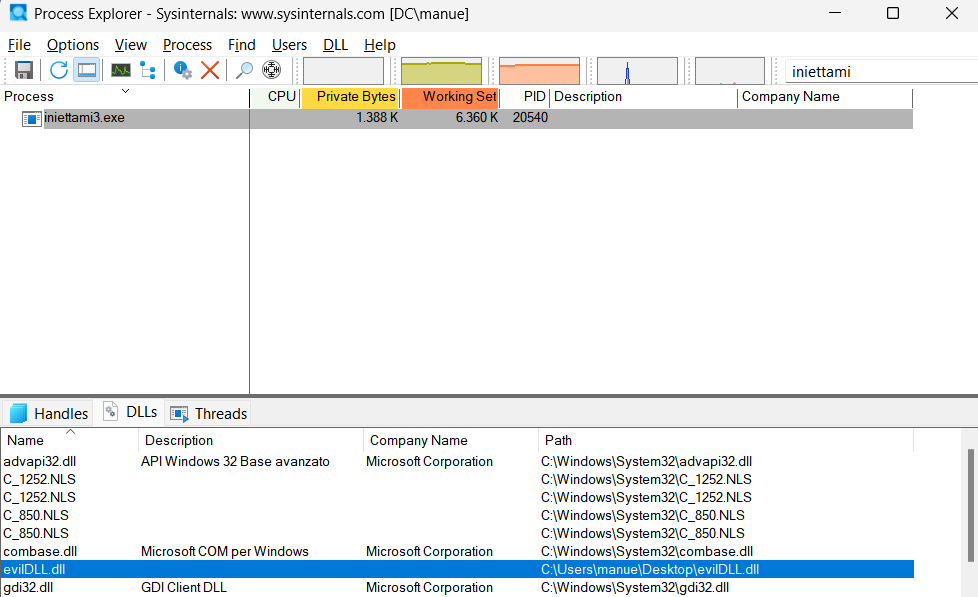
\includegraphics[width=\textwidth,height=7cm]{res/fig/hook-dll.png}
    \caption{DLL all'interno del processo monitorato.}
    \label{fig:hook1}
\end{figure}

\begin{figure}[hbtp]
    \centering
    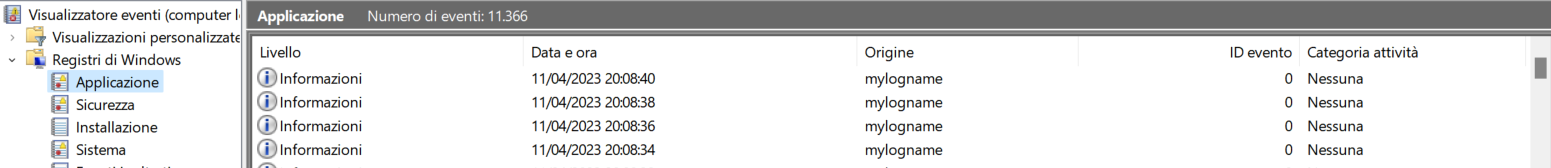
\includegraphics[width=\textwidth]{res/fig/hook-evento.png}
    \caption{generazione di evento in Windows Event Log System.}
    \label{fig:hook2}
\end{figure}
\begin{figure}[hbtp]
    \centering
    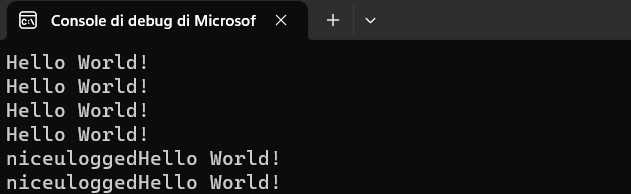
\includegraphics[width=\textwidth,height=5cm]{res/fig/hook-console.png}
    \caption{console del processo prima e dopo l'hook.}
    \label{fig:hook3}
\end{figure}